\documentclass{beamer}
\usetheme{Madrid}
\beamertemplatenavigationsymbolsempty

% Enable non-ugly hyperlinks
\usepackage{blindtext}
\usepackage{epigraph}
\usepackage{multicol}

\usepackage{dsfont}
\usepackage{stmaryrd}
\usepackage{colortbl}
\usepackage{hyperref}

\usepackage{amsmath}
\DeclareMathOperator*{\argmax}{argmax}
\DeclareMathOperator*{\argmin}{argmin}
\usepackage{amssymb}

\usepackage[dvipsnames, table]{xcolor}
\usepackage{textcomp}

% Packages
\usepackage[pdf]{graphviz}
\usepackage{mathrsfs}

\newcommand*\circled[1]{\tikz[baseline=-0.1cm]{
  \node[shape=circle,draw,inner sep=0.48pt] (char) {\fontsize{7}{12}\textsf{#1}};}}

\DeclareMathAlphabet{\mathcal}{OMS}{cmsy}{m}{n}
\usepackage{cancel}
\newcommand\ccancel[2][red]{\renewcommand\CancelColor{\color{#1}}\cancel{#2}}
\newcommand{\nDownarrow}{\ensuremath{\text{ }\cancel{\Downarrow}\text{ }}}
\usepackage{centernot}

\usepackage{pgfplots, pgfplotstable}
\pgfplotsset{compat=1.7}
\usepgfplotslibrary{fillbetween}
\usetikzlibrary{patterns}
\pgfmathdeclarefunction{gauss}{2}{\pgfmathparse{1/(#2*sqrt(2*pi))*exp(-((x-#1)^2)/(2*#2^2))}}
\pgfmathdeclarefunction{nil}{1}{\pgfmathparse{0.001}}

\usepackage{arydshln}
\usepackage{adjustbox}
\usepackage{enumerate}
\usepackage{enumitem}
\usepackage{tikz-cd}
\usetikzlibrary{calc}
\usepackage{amsfonts}
%\usepackage{prooftrees}
\usepackage{bussproofs}
\renewcommand{\sectionautorefname}{\S}
\renewcommand{\subsectionautorefname}{\S}
\usepackage{float}

\usepackage{tikz-3dplot}
\usetikzlibrary{3d}
\usetikzlibrary{calligraphy}
\newif\ifshowcellnumber
\showcellnumbertrue

\usepackage{algorithm}
\usepackage[noend]{algpseudocode}
\usepackage{algorithmicx}
\usepackage{sourcecodepro}
\usepackage{tikz-qtree}
\usepackage{amsthm}
\usepackage{bm}
\usetikzlibrary{bayesnet}
\usetikzlibrary{arrows}
\usepackage{subcaption}
\usetikzlibrary{backgrounds}
\usetikzlibrary{tikzmark}
\usetikzlibrary{hobby}

\usepackage{mwe}

\newcommand{\E}{\mathbb{E}}
\newcommand{\Var}{\mathrm{Var}}
\newcommand{\Cov}{\mathrm{Cov}}

\newcommand{\CompOrder}{\mathcal{O}}
\def\graphspace{\mathbf{G}}
\def\Uniform{\mbox{\rm Uniform}}
\def\Gaussian{\mbox{\rm Gaussian}}
\def\Bernoulli{\mbox{\rm Bernoulli}}
\def\Dirichlet{\mbox{\rm Dirichlet}}

\usepackage{mathtools}% superior to amsmath
\usepackage{tikz}
% Packages
\usepackage{listings}
\DeclareRobustCommand{\hlred}[1]{{\sethlcolor{pink}\hl{#1}}}
\usepackage{fontspec}

\setmonofont[Scale=0.8]{JetBrainsMono}[
  Contextuals={Alternate},
  Path=./font/,
  Extension = .ttf,
  UprightFont=*-Regular,
  BoldFont=*-Bold,
  ItalicFont=*-Italic,
  BoldItalicFont=*-BoldItalic
]

\usepackage[skins,breakable,listings]{tcolorbox}

\lstdefinelanguage{python}{
  comment=[l]{//},
  commentstyle={\color{gray}\ttfamily},
  emph={delegate, filter, firstOrNull, forEach, it, lazy, mapNotNull, println, repeat, assert, with, head, tail, len, return@},
  numberstyle=\noncopyable,
  identifierstyle=\color{black},
  keywords={abstract, actual, as, as?, break, by, class, companion, continue, data, do, dynamic, else, enum, expect, false, final, for, fun, get, if, import, in, infix, interface, internal, is, null, object, open, operator, override, package, private, public, return, sealed, set, super, suspend, this, throw, true, try, catch, typealias, val, var, vararg, when, where, while, tailrec, reified, from, import, def, yield, lambda, as, in, return, else, pass},
  keywordstyle={\bfseries},
  morecomment=[s]{/*}{*/},
  morestring=[b]",
  morestring=[s]{"""*}{*"""},
  ndkeywords={@Deprecated, @JvmField, @JvmName, @JvmOverloads, @JvmStatic, @JvmSynthetic, Array, Byte, Double, Float, Boolean, Int, Integer, Iterable, Long, Runnable, Short, String, int},
  ndkeywordstyle={\bfseries},
  sensitive=true,
  stringstyle={\ttfamily},
  literate={`}{{\char0}}1,
  escapeinside={(*@}{@*)}
}

\lstnewenvironment{smallpy}
{\lstset{
  basicstyle=\ttfamily\lst@ifdisplaystyle\footnotesize\fi,
  language=python
}}
{}

\lstdefinelanguage{tidy}{
  comment=[l]{//},
  commentstyle={\color{gray}\ttfamily},
  emph={|, ->, ---},
  emphstyle={\color{red}},
  identifierstyle=\color{black},
  keywords={\|, ->, ---},
  otherkeywords={|,->},
  morekeywords={|,->},
  keywordstyle={\color{blue}\bfseries},
  morecomment=[s]{/*}{*/},
  morestring=[b]",
  morestring=[s]{"""*}{*"""},
  ndkeywords={@Deprecated, @JvmField, @JvmName, @JvmOverloads, @JvmStatic, @JvmSynthetic, Array, Byte, Double, Float, Int, Integer, Iterable, Long, Runnable, Short, String},
  ndkeywordstyle={\color{orange}\bfseries},
  sensitive=true,
  stringstyle={\color{green}\ttfamily},
  literate={`}{{\char0}}1
}

%%%%%%%%%%%%%%%%%%%%%%%%%%%%%%%%%%%%%%%%%%%
%
% Color boxes
%
%%%%%%%%%%%%%%%%%%%%%%%%%%%%%%%%%%%%%%%%%%%

\tcbset{
  enhanced jigsaw,
  breakable,
  listing only,
%  boxsep=-1pt,
%  top=-1pt,
  bottom=0.1cm,
  right=0.5cm,
  overlay first={
    \node[black!50] (S) at (frame.south) {\Large\ding{34}};
    \draw[dashed,black!50] (frame.south west) -- (S) -- (frame.south east);
  },
  overlay middle={
    \node[black!50] (S) at (frame.south) {\Large\ding{34}};
    \draw[dashed,black!50] (frame.south west) -- (S) -- (frame.south east);
    \node[black!50] (S) at (frame.north) {\Large\ding{34}};
    \draw[dashed,black!50] (frame.north west) -- (S) -- (frame.north east);
  },
  overlay last={
    \node[black!50] (S) at (frame.north) {\Large\ding{34}};
    \draw[dashed,black!50] (frame.north west) -- (S) -- (frame.north east);
  },
  before={\par\vspace{5pt}},
  after={\par\vspace{\parskip}\noindent}
}

\definecolor{slightgray}{rgb}{0.90, 0.90, 0.90}

\usepackage{soul}
\makeatletter
\def\SOUL@hlpreamble{%
  \setul{}{3.0ex}%
  \let\SOUL@stcolor\SOUL@hlcolor%
  \SOUL@stpreamble%
}
\makeatother

\newcommand{\inline}[1]{%
  \begingroup%
  \sethlcolor{slightgray}%
  \hl{\ttfamily\footnotesize #1}%
  \endgroup
}

\newcommand{\tinline}[1]{%
  \begingroup%
  \sethlcolor{slightgray}%
  \hl{\ttfamily\tiny #1}%
  \endgroup
}

\newtcblisting{halftidyinput}[1][]{%
  left skip=0.7cm,
  left=0.35cm,
  width=6cm,
%  left=-0.01cm,
  top=-0.1cm,
  bottom=-0.35cm,
  listing options={
    language=tidy,
    basicstyle=\ttfamily\small,
%numberstyle=\footnotesize,
    showstringspaces=false,
    tabsize=2,
    breaklines=true,
    numbers=none,
    inputencoding=utf8,
    escapeinside={(*@}{@*)},
    #1
  },
  underlay unbroken and first={%
    \path[draw=none] (interior.north west) rectangle node[white]{\includegraphics[width=4mm]{../figures/tidyparse_logo.png}} ([xshift=-10mm,yshift=-7mm]interior.north west);
  }
}

\newtcblisting{wholetidyinput}[1][]{%
  left skip=0.7cm,
  left=0.35cm,
  top=0.1cm,
  middle=0mm,
  boxsep=0mm,
  listing options={
    language=tidy,
    basicstyle=\ttfamily\small,
%numberstyle=\footnotesize,
    showstringspaces=false,
    tabsize=2,
    breaklines=true,
    numbers=none,
    inputencoding=utf8,
    escapeinside={(*@}{@*)},
    #1
  },
  underlay unbroken and first={%
    \path[draw=none] (interior.north west) rectangle node[white]{\includegraphics[width=4mm]{../figures/tidyparse_logo.png}} ([xshift=-10mm,yshift=-9mm]interior.north west);
  }
}

\definecolor{A}{RGB}{6,150,104}
\definecolor{B}{RGB}{196,74,137}
\definecolor{C}{RGB}{117,237,133}
\definecolor{D}{RGB}{246,46,243}
\definecolor{E}{RGB}{89,162,12}
\definecolor{F}{RGB}{113,12,158}
\definecolor{G}{RGB}{191,205,142}
\definecolor{H}{RGB}{51,58,158}
\definecolor{I}{RGB}{244,212,3}
\definecolor{J}{RGB}{37,36,249}
\definecolor{K}{RGB}{253,165,71}
\definecolor{L}{RGB}{27,81,29}
\colorlet{LA}{A!30}
\colorlet{LB}{B!30}
\colorlet{LC}{C!30}
\colorlet{LD}{D!30}
\colorlet{LE}{E!30}
\colorlet{LF}{F!30}
\colorlet{LG}{G!30}
\colorlet{LH}{H!30}
\colorlet{LI}{I!30}
\colorlet{LJ}{J!30}
\colorlet{LK}{K!30}
\colorlet{LL}{L!30}
\newcommand{\hiliA}[1]{%
  \colorbox{LA}{$#1$}}
\newcommand{\hiliB}[1]{%
  \colorbox{LB}{$#1$}}
\newcommand{\hiliC}[1]{%
  \colorbox{LC}{$#1$}}
\newcommand{\hiliD}[1]{%
  \colorbox{LD}{$#1$}}
\newcommand{\hiliE}[1]{%
  \colorbox{LE}{$#1$}}
\newcommand{\hiliF}[1]{%
  \colorbox{LF}{$#1$}}
\newcommand{\hiliG}[1]{%
  \colorbox{LG}{$#1$}}
\newcommand{\hiliH}[1]{%
  \colorbox{LH}{$#1$}}
\newcommand{\hiliI}[1]{%
  \colorbox{LI}{$#1$}}
\newcommand{\hiliJ}[1]{%
  \colorbox{LJ}{$#1$}}
\newcommand{\hiliK}[1]{%
  \colorbox{LK}{$#1$}}
\newcommand{\hiliL}[1]{%
  \colorbox{LL}{$#1$}}
\newcommand{\highlight}[1]{%
  \colorbox{lgray}{$#1$}}
\colorlet{lred}{red!30}
\colorlet{lorange}{orange!30}
\colorlet{lgreen}{green!30}
\colorlet{lgray}{black!15}
\colorlet{dgray}{black!75}
\DeclareRobustCommand{\hlred}[1]{{\sethlcolor{lred}\hl{#1}}}
\DeclareRobustCommand{\hlorange}[1]{{\sethlcolor{lorange}\hl{#1}}}
\DeclareRobustCommand{\hlgreen}[1]{{\sethlcolor{lgreen}\hl{#1}}}
\DeclareRobustCommand{\hlgray}[1]{{\sethlcolor{lgray}\hl{#1}}}
\DeclareRobustCommand{\caret}[1]{{\sethlcolor{dgray}\textcolor{white}{\hl{#1}}}}

\usepackage{url}
\usepackage{qtree}

\usepackage{filecontents}
\usepackage{pstricks-add}
\usepackage{emoji}
\usepackage{alltt}
\usepackage{nicematrix}
\usepackage{graphicx}
\usepackage{ulem}
\usepackage{upquote}
\tikzstyle{every picture}+=[remember picture]
\usepackage{menukeys}
\pgfplotstableread[col sep=comma,]{timings_loc.csv}\loctimings
\pgfplotstableread[col sep=comma,]{timings_unloc.csv}\unloctimings

\makeatletter
\DeclareRobustCommand{\cev}[1]{%
    {\mathpalette\do@cev{#1}}%
}
\newcommand{\do@cev}[2]{%
  \vbox{\offinterlineskip
  \sbox\z@{$\m@th#1 x$}%
  \ialign{##\cr
  \hidewidth\reflectbox{$\m@th#1\vec{}\mkern4mu$}\hidewidth\cr
  \noalign{\kern-\ht\z@}
    $\m@th#1#2$\cr
  }%
  }%
}
\makeatother

\makeatletter
\DeclareRobustCommand{\pder}[1]{%
  \@ifnextchar\bgroup{\@pder{#1}}{\@pder{}{#1}}}
\newcommand{\@pder}[2]{\frac{\partial#1}{\partial#2}}
\makeatother

\newcommand{\shup}{\shortuparrow}
\newcommand{\shri}{\shortrightarrow}
\newcommand{\shur}{\shup\hspace{-5pt}\shri}

\makeatletter
\def\squigglyred{\bgroup \markoverwith{\textcolor{red}{\lower3\p@\hbox{\sixly \char58}}}\ULon}
\makeatother

\makeatletter
\def\squigglyblu{\bgroup \markoverwith{\textcolor{blue}{\lower3\p@\hbox{\sixly \char58}}}\ULon}
\makeatother

\makeatletter
\def\squigglyora{\bgroup \markoverwith{\textcolor{orange}{\lower3\p@\hbox{\sixly \char58}}}\ULon}
\makeatother

\newcommand{\err}[1]{\smash{\squigglyred{#1}{}}}
\newcommand{\erb}[1]{\smash{\squigglyblu{#1}{}}}
\newcommand{\ero}[1]{\smash{\squigglyora{#1}{}}}
\newcommand{\stirlingii}{\genfrac{\{}{\}}{0pt}{}}

%======== Arrows =========
\newcommand{\knightarrow}{
  \tikz{
    \fill (0pt,0pt) circle [radius = 1pt];
    \fill (0pt,6pt) circle [radius = 1pt];
    \fill (6pt,0pt) circle [radius = 1pt];
    \fill (6pt,6pt) circle [radius = 1pt];
    \fill (12pt,0pt) circle [radius = 1pt];
    \fill (12pt,6pt) circle [radius = 1pt];
    \fill (6pt,0pt) circle [radius = 1pt];
    \fill (12pt,0pt) circle [radius = 1pt];
    \draw [-to] (0pt,0pt) -- (12pt,6pt);
  }
}

\newcommand{\kingarrow}{
  \tikz{
    \fill (0pt,0pt) circle [radius = 1pt];
    \fill (6pt,0pt) circle [radius = 1pt];
    \fill (0pt,6pt) circle [radius = 1pt];
    \fill (6pt,6pt) circle [radius = 1pt];
    \draw [-to] (0pt,0pt) -- (6pt,6pt);
    \draw [-to] (0pt,0pt) -- (0pt,6pt);
    \draw [-to] (0pt,0pt) -- (6pt,0pt);
  }
}

\newcommand{\duparrow}{
  \tikz{
    \fill[white] (0pt,0pt) circle [radius = 1pt];
    \fill (6pt,0pt) circle [radius = 1pt];
    \fill (0pt,6pt) circle [radius = 1pt];
    \fill[white] (6pt,6pt) circle [radius = 1pt];
    \draw [-to] (6pt,0pt) -- (0pt,6pt);
  }
}

\newcommand{\drightarrow}{
  \tikz{
    \fill (0pt,0pt) circle [radius = 1pt];
    \fill (6pt,0pt) circle [radius = 1pt];
    \draw [-to] (0pt,0pt) -- (6pt,0pt);
  }
}

\newcommand{\ddiagarrow}{
  \tikz{
    \fill (0pt,0pt) circle [radius = 1pt];
    \fill (6pt,0pt) circle [radius = 1pt];
    \fill (0pt,6pt) circle [radius = 1pt];
    \fill (6pt,6pt) circle [radius = 1pt];
    \draw [-to] (0pt,0pt) -- (6pt,6pt);
  }
}

\newcommand{\knightkingarrow}{
  \tikz{
    \fill (0pt,0pt) circle [radius = 1pt];
    \fill (0pt,6pt) circle [radius = 1pt];
    \fill (6pt,0pt) circle [radius = 1pt];
    \fill (6pt,6pt) circle [radius = 1pt];
    \fill (12pt,0pt) circle [radius = 1pt];
    \fill (12pt,6pt) circle [radius = 1pt];
    \draw [-to] (0pt,0pt) -- (6pt,6pt);
    \draw [-to] (0pt,0pt) -- (0pt,6pt);
    \draw [-to] (0pt,0pt) -- (6pt,0pt);
    \draw [-to] (0pt,0pt) -- (12pt,6pt);
  }
}

%======== Arrows =========

\usetikzlibrary{decorations.pathreplacing,automata,calc,positioning,matrix,chains,fit,decorations.pathmorphing}

\usepackage{wrapfig}

\newcommand{\mkTrellis}[1]{
  \begin{tikzpicture}
  \def\dx{20pt}
  \def\dy{30pt}
  \newcounter{i}
  \stepcounter{i}
  \node[circle, draw, fill=black!30] (\arabic{i}) at (0,0){};
  \foreach [count=\i] \x in {2,...,#1}{
    \pgfmathsetmacro{\lox}{\x-1}%
    \pgfmathsetmacro{\loxt}{\x-3}%
    \foreach [count=\j] \xx in {-\lox,-\loxt,...,\lox}{
      \pgfmathsetmacro{\jj}{\j-1}%
      \stepcounter{i}
      \pgfmathsetmacro{\kk}{\xx-2}%
      \pgfmathsetmacro{\lbl}{\lox!/(\jj!*(\lox-\jj)!)}
      \ifnum\x<\kk
      \pgfmath\node[circle, draw]  (\arabic{i}) at (\xx*\dx, -\lox*\dy) {};
      \else
        \pgfmath\node[circle, draw, fill=black!30]  (\arabic{i}) at (\xx*\dx, -\lox*\dy) {};
      \fi
    }
  }
  \newcounter{z}
  \newcounter{xn}
  \newcounter{xnn}
  \pgfmathsetmacro{\maxx}{#1 - 1}
  \foreach \x in {1,...,\maxx}{
    \foreach \xx in {1,...,\x}{
      \stepcounter{z}
      \setcounter{xn}{\arabic{z}}
      \addtocounter{xn}{\x}
      \setcounter{xnn}{\arabic{xn}}
      \stepcounter{xnn}
      \draw [<-] (\arabic{z}) -- (\arabic{xn});
      \draw [<-] (\arabic{z}) -- (\arabic{xnn});
    }
  }
  \end{tikzpicture}
}

\newcommand{\dx}{20pt}
\newcommand{\dy}{30pt}
\newcounter{i}
\newcounter{z}
\newcounter{xn}
\newcounter{xnn}
\newcommand{\mkTrellisAppend}[1]{
  \begin{tikzpicture}
  \setcounter{i}{0}
  \setcounter{z}{0}
  \setcounter{xn}{0}
  \setcounter{xnn}{0}
  \stepcounter{i}
  \node[circle, draw] (\arabic{i}) at (0,0){};
  \foreach [count=\i] \x in {2,...,#1}{
    \pgfmathsetmacro{\lox}{\x-1}%
    \pgfmathsetmacro{\loxt}{\x-3}%
    \foreach [count=\j] \xx in {-\lox,-\loxt,...,\lox}{
      \pgfmathsetmacro{\jj}{\j-1}%
      \stepcounter{i}
      \pgfmathsetmacro{\kk}{\xx+2}%
      \pgfmathsetmacro{\lbl}{\lox!/(\jj!*(\lox-\jj)!)}
      \ifnum\x>\kk
      \pgfmath\node[circle, draw, fill=black!30]  (\arabic{i}) at (\xx*\dx, -\lox*\dy) {};
      \else
        \pgfmath\node[circle, draw]  (\arabic{i}) at (\xx*\dx, -\lox*\dy) {};
      \fi
    }
  }
  \pgfmathsetmacro{\maxx}{#1 - 1}
  \foreach \x in {1,...,\maxx}{
    \foreach \xx in {1,...,\x}{
      \stepcounter{z}
      \setcounter{xn}{\arabic{z}}
      \addtocounter{xn}{\x}
      \setcounter{xnn}{\arabic{xn}}
      \stepcounter{xnn}
      \draw [<-] (\arabic{z}) -- (\arabic{xn});
      \draw [<-] (\arabic{z}) -- (\arabic{xnn});
    }
  }
  \end{tikzpicture}
}

\newcommand{\mkTrellisInsert}[1]{
  \begin{tikzpicture}
  \setcounter{i}{0}
  \setcounter{z}{0}
  \setcounter{xn}{0}
  \setcounter{xnn}{0}
  \stepcounter{i}
  \node[circle, draw] (\arabic{i}) at (0,0){};
  \foreach [count=\i] \x in {2,...,#1}{
    \pgfmathsetmacro{\lox}{\x-1}%
    \pgfmathsetmacro{\loxt}{\x-3}%
    \foreach [count=\j] \xx in {-\lox,-\loxt,...,\lox}{
      \pgfmathsetmacro{\jj}{\j-1}%
      \stepcounter{i}
      \pgfmathsetmacro{\mp}{\xx+#1}%
      \pgfmathsetmacro{\mq}{\xx+\x}%
      \pgfmathsetmacro{\lbl}{\lox!/(\jj!*(\lox-\jj)!)}
      \ifnum\x>\mp
      \pgfmath\node[circle, draw, fill=black!30]  (\arabic{i}) at (\xx*\dx, -\lox*\dy) {};
      \else
        \ifnum#1<\mq
        \pgfmath\node[circle, draw, fill=black!30]  (\arabic{i}) at (\xx*\dx, -\lox*\dy) {};
        \else
          \pgfmath\node[circle, draw]  (\arabic{i}) at (\xx*\dx, -\lox*\dy) {};
        \fi
      \fi

    }
  }
  \pgfmathsetmacro{\maxx}{#1 - 1}
  \foreach \x in {1,...,\maxx}{
    \foreach \xx in {1,...,\x}{
      \stepcounter{z}
      \setcounter{xn}{\arabic{z}}
      \addtocounter{xn}{\x}
      \setcounter{xnn}{\arabic{xn}}
      \stepcounter{xnn}
      \draw [<-] (\arabic{z}) -- (\arabic{xn});
      \draw [<-] (\arabic{z}) -- (\arabic{xnn});
    }
  }
  \end{tikzpicture}
}

\usetikzlibrary{automata, positioning, arrows}

\newcommand{\nobarfrac}{\genfrac{}{}{0pt}{}}
\pgfplotstableread[col sep=comma,]{timings_loc.csv}\loctimings
\pgfplotstableread[col sep=comma,]{timings_unloc.csv}\unloctimings
\pgfplotstableread[col sep=comma,]{natural_errors.csv}\naturalerrors
\pgfplotstableread[col sep=comma,]{synthetic_errors.csv}\syntheticerrors

\usepackage[all,pdf]{xy}

\newcommand{\bs}{\blacksquare}
\newcommand{\ws}{\square}

\usepackage{multicol}
\usetikzlibrary{shapes.geometric, arrows}

\tikzstyle{startstop} = [rectangle, rounded corners,
minimum width=3cm,
minimum height=1cm,
thick,
text centered,
draw=none,
]

\tikzstyle{plain} = [
rectangle,
rounded corners,
minimum width=3.5cm,
minimum height=1cm,
thick,
text centered,
draw=black
]

\tikzstyle{io} = [trapezium,
trapezium stretches=true, % A later addition
thick,
trapezium left angle=70,
trapezium right angle=110,
minimum width=3cm,
minimum height=1cm, text centered,
draw=black, fill=blue!30]

\tikzstyle{io2} = [trapezium,
trapezium stretches=true, % A later addition
thick,
trapezium left angle=70,
trapezium right angle=110,
minimum width=3cm,
minimum height=1cm, text centered,
draw=black, fill=black!30]

\tikzstyle{process} = [rectangle,
minimum width=3.5cm,
minimum height=1cm,
thick,
text centered,
text width=4cm,
draw=black,
fill=orange!30]

\tikzstyle{decision} = [diamond,
minimum width=2.5cm,
minimum height=0.5cm,
thick,
text centered,
draw=black,
fill=green!30]
\tikzstyle{arrow} = [->,thick]

%\usetikzlibrary{external}
%\tikzexternalize[prefix=figures/]
\definecolor{green}{RGB}{0,128,0}
\definecolor{darkgray176}{RGB}{176,176,176}
\definecolor{darkviolet1270255}{RGB}{127,0,255}
\definecolor{deepskyblue3176236}{RGB}{3,176,236}
\definecolor{dodgerblue45123246}{RGB}{45,123,246}
\definecolor{lightgray204}{RGB}{204,204,204}
\definecolor{royalblue8762253}{RGB}{87,62,253}

\usepackage{sankey}

\usepackage{pgf-soroban}
\usetikzlibrary{shapes.geometric,calc,decorations.text,bayesnet,arrows,backgrounds}
\usepackage{circledsteps}
\usepackage{epigraph}
\usepackage{array}
\setmonofont{JetBrains Mono}[
  Contextuals = Alternate,
  Ligatures = TeX,
]
\lstset{
  basicstyle = \ttfamily,
  columns = flexible,
}
\makeatletter
\renewcommand*\verbatim@nolig@list{}
\makeatother
\usepackage{pmboxdraw}
\usetikzlibrary{cd}
\usepackage{pifont}
\newcommand{\cmark}{\ding{51}}%
\newcommand{\xmark}{\ding{55}}%

\setbeamertemplate{footline}
{
  \leavevmode%
  \hbox{%
    \begin{beamercolorbox}[wd=.25\paperwidth,ht=2.25ex,dp=1ex,center]{author in head/foot}%
      \usebeamerfont{author in head/foot}\insertshortauthor{}{~~(\insertshortinstitute)}
    \end{beamercolorbox}%
    \begin{beamercolorbox}[wd=.5\paperwidth,ht=2.25ex,dp=1ex,center]{title in head/foot}%
      \usebeamerfont{title in head/foot}\insertshorttitle
    \end{beamercolorbox}%
    \begin{beamercolorbox}[wd=.3\paperwidth,ht=2.25ex,dp=1ex,right]{date in head/foot}%
      \usebeamerfont{date in head/foot}\insertshortdate{}\hspace*{2em}
      \insertframenumber{} / \inserttotalframenumber\hspace*{2ex}
    \end{beamercolorbox}}%
  \vskip0pt%
}
\makeatother

\makeatletter
\let\HL\hl
\renewcommand\hl{%
  \let\set@color\beamerorig@set@color
  \let\reset@color\beamerorig@reset@color
  \HL}
\makeatother

\newcommand{\ddd}{\Ddots}
\newcommand{\vdd}{\Vdots}
\newcommand{\cdd}{\Cdots}
\newcommand{\lds}{\ldots}
\newcommand{\vno}{\varnothing}
\newcommand{\ts}[1]{\textsuperscript{#1}}
\newcommand{\non}{1\ts{st}}
\newcommand{\ntw}{2\ts{nd}}
\newcommand{\nth}{3\ts{rd}}
\newcommand{\nfo}{4\ts{th}}
\newcommand{\nfi}{5\ts{th}}
\newcommand{\nsi}{6\ts{th}}
\newcommand{\nse}{7\ts{th}}
\newcommand{\vs}[1]{\sigma_{#1}^{\shur}}
\newcommand{\rcr}{\rowcolor{black!15}}
\newcommand{\rcw}{\rowcolor{white}}
\newcommand{\pcd}{\cdot}
\newcommand{\pcp}{\phantom\cdot}
\newcommand{\ppp}{\phantom{\nse}}
\newcommand{\hole}{\underline{\hspace{0.25cm}}}

\title[Syntax Repair as Language Intersection]{Repairing Multiline Syntax Errors\\Using the Levenshtein-Bar-Hillel Construction}
\titlegraphic{\includegraphics[width=0.2\textwidth]{../figures/tidyparse_logo}}
\author[Considine, Guo, Si]{\textbf{Breandan Considine}, Jin Guo, Xujie Si}
\institute[McGill]{
  McGill University, Mila IQIA\\
  \medskip
  \textit{bre@ndan.co}
}
\date{\today}

\begin{document}
\begin{frame}
  \titlepage
\end{frame}

\begin{frame}{Overview}
  \tableofcontents
\end{frame}

\begin{frame}[fragile]{Can you spot the error?}
  \begin{center}
    \begin{tabular}{|m{5.5cm}|m{5.5cm}|}
      \hline \rule{0pt}{2.5ex}\textbf{Original code}\rule[-1ex]{0pt}{2ex} &  \rule{0pt}{2.5ex}\textbf{Human repair}\rule[-1ex]{0pt}{2ex} \\\hline
      \begin{lstlisting}[escapechar=!, basicstyle=\linespread{1.3}\ttfamily\footnotesize]

  newlist = []
  i = set([5, 3, 1)]
  z = set([5, 0, 4)]


      \end{lstlisting} & \begin{lstlisting}[escapechar=!, basicstyle=\linespread{1.3}\ttfamily\footnotesize]

      \end{lstlisting} \\\hline
    \end{tabular}
  \end{center}
\end{frame}

\begin{frame}[fragile]{Can you spot the error?}
  \begin{center}
    \begin{tabular}{|m{5.5cm}|m{5.5cm}|}
      \hline \rule{0pt}{2.5ex}\textbf{Original code}\rule[-1ex]{0pt}{2ex} &  \rule{0pt}{2.5ex}\textbf{Human repair}\rule[-1ex]{0pt}{2ex} \\\hline
      \begin{lstlisting}[escapechar=!, basicstyle=\linespread{1.3}\ttfamily\footnotesize]

  newlist = []
  i = set([5, 3, 1)]
  z = set([5, 0, 4)]

      \end{lstlisting} & \begin{lstlisting}[escapechar=!, basicstyle=\linespread{1.3}\ttfamily\footnotesize]

  newlist = []
  i = set([5, 3, 1!\hlorange{])}!
  z = set([5, 0, 4!\hlorange{])}!

      \end{lstlisting} \\\hline
    \end{tabular}
  \end{center}
\end{frame}

\begin{frame}[fragile]{Can you spot the error?}
  \begin{center}
    \begin{tabular}{|m{5.5cm}|m{5.5cm}|}
      \hline \rule{0pt}{2.5ex}\textbf{Original code}\rule[-1ex]{0pt}{2ex} &  \rule{0pt}{2.5ex}\textbf{Human repair}\rule[-1ex]{0pt}{2ex} \\\hline
      \begin{lstlisting}[escapechar=!, basicstyle=\linespread{1.3}\ttfamily\footnotesize]

  def average(values):
    if values == (1,2,3):
      return (1+2+3)/3
    else if values == (-3,2):
      return (-3+2+8-1)/4

      \end{lstlisting} & \begin{lstlisting}[escapechar=!, basicstyle=\linespread{1.3}\ttfamily\footnotesize]

      \end{lstlisting} \\\hline
    \end{tabular}
  \end{center}
\end{frame}

\begin{frame}[fragile]{Can you spot the error?}
  \begin{center}
    \begin{tabular}{|m{5.5cm}|m{5.5cm}|}
      \hline \rule{0pt}{2.5ex}\textbf{Original code}\rule[-1ex]{0pt}{2ex} &  \rule{0pt}{2.5ex}\textbf{Human repair}\rule[-1ex]{0pt}{2ex} \\\hline
      \begin{lstlisting}[escapechar=!, basicstyle=\linespread{1.3}\ttfamily\footnotesize]

  def average(values):
    if values == (1,2,3):
      return (1+2+3)/3
    !\hlorange{else}! !\hlred{if}! values == (-3,2):
      return (-3+2+8-1)/4

      \end{lstlisting} & \begin{lstlisting}[escapechar=!, basicstyle=\linespread{1.3}\ttfamily\footnotesize]

  def average(values):
    if values == (1,2,3):
      return (1+2+3)/3
    !\hlorange{elif}! values == (-3,2):
      return (-3+2+8-1)/4

      \end{lstlisting} \\\hline
    \end{tabular}
  \end{center}
\end{frame}

\begin{frame}[fragile]{Can you spot the error?}
  \begin{center}
    \begin{tabular}{|m{5.5cm}|m{5.5cm}|}
      \hline \rule{0pt}{2.5ex}\textbf{Original code}\rule[-1ex]{0pt}{2ex} &  \rule{0pt}{2.5ex}\textbf{Human repair}\rule[-1ex]{0pt}{2ex} \\\hline
      \begin{lstlisting}[escapechar=!, basicstyle=\linespread{1.3}\ttfamily\footnotesize]

  import Global from Global
  globalObj = Global()
  print(str(globalObj.Test()))

      \end{lstlisting} & \begin{lstlisting}[escapechar=!, basicstyle=\linespread{1.3}\ttfamily\footnotesize]

      \end{lstlisting} \\\hline
    \end{tabular}
  \end{center}
\end{frame}

\begin{frame}[fragile]{Can you spot the error?}
  \begin{center}
    \begin{tabular}{|m{5.5cm}|m{5.5cm}|}
      \hline \rule{0pt}{2.5ex}\textbf{Original code}\rule[-1ex]{0pt}{2ex} &  \rule{0pt}{2.5ex}\textbf{Human repair}\rule[-1ex]{0pt}{2ex} \\\hline
      \begin{lstlisting}[escapechar=!, basicstyle=\linespread{1.3}\ttfamily\footnotesize]

  !\hlorange{import}! Global !\hlorange{from}! Global
  globalObj = Global()
  print(str(globalObj.Test()))

      \end{lstlisting} & \begin{lstlisting}[escapechar=!, basicstyle=\linespread{1.3}\ttfamily\footnotesize]

  !\hlorange{from}! Global !\hlorange{import}! Global
  globalObj = Global()
  print(str(globalObj.Test()))

      \end{lstlisting} \\\hline
    \end{tabular}
  \end{center}
\end{frame}

%\begin{frame}[fragile]{Can you spot the error?}
%  \begin{center}
%    \begin{tabular}{|m{5.5cm}|m{5.5cm}|}
%      \hline \rule{0pt}{2.5ex}\textbf{Original code}\rule[-1ex]{0pt}{2ex} &  \rule{0pt}{2.5ex}\textbf{Human repair}\rule[-1ex]{0pt}{2ex} \\\hline
%      \begin{lstlisting}[escapechar=!, basicstyle=\linespread{1.3}\ttfamily\footnotesize]
%
%   try:
%     something()
%   catch AttributeError:
%     pass
%
%      \end{lstlisting} & \begin{lstlisting}[escapechar=!, basicstyle=\linespread{1.3}\ttfamily\footnotesize]
%
%      \end{lstlisting} \\\hline
%    \end{tabular}
%  \end{center}
%\end{frame}
%
%\begin{frame}[fragile]{Can you spot the error?}
%  \begin{center}
%    \begin{tabular}{|m{5.5cm}|m{5.5cm}|}
%      \hline \rule{0pt}{2.5ex}\textbf{Original code}\rule[-1ex]{0pt}{2ex} &  \rule{0pt}{2.5ex}\textbf{Human repair}\rule[-1ex]{0pt}{2ex} \\\hline
%      \begin{lstlisting}[escapechar=!, basicstyle=\linespread{1.3}\ttfamily\footnotesize]
%
%   try:
%     something()
%   !\hlorange{catch}! AttributeError:
%     pass
%
%      \end{lstlisting} & \begin{lstlisting}[escapechar=!, basicstyle=\linespread{1.3}\ttfamily\footnotesize]
%
%   try:
%     something()
%   !\hlorange{except}! AttributeError:
%     pass
%
%      \end{lstlisting} \\\hline
%    \end{tabular}
%  \end{center}
%\end{frame}

\begin{frame}[t,fragile]{How many repairs could there possibly be?}
  Consider the following Python snippet, which contains a small syntax error:\\

  \begin{lstlisting}[escapechar=!, basicstyle=\linespread{1.3}\ttfamily\footnotesize]
    def prepend(i, k, L=[])
      n and [prepend(i - 1, k, [b] + L) for b in range(k)]
  \end{lstlisting}
\end{frame}

\begin{frame}[t,fragile]{How many repairs could there possibly be?}
  Consider the following Python snippet, which contains a small syntax error:\\

  \begin{lstlisting}[escapechar=!, basicstyle=\linespread{1.3}\ttfamily\footnotesize]
    def prepend(i, k, L=[])
      n and [prepend(i - 1, k, [b] + L) for b in range(k)]
  \end{lstlisting}

  It can be fixed by appending a colon after the function signature, yielding:\\

    \begin{lstlisting}[escapechar=!, basicstyle=\linespread{1.3}\ttfamily\footnotesize]
    def prepend(i, k, L=[])!\hlgreen{:}!
      n and [prepend(i - 1, k, [b] + L) for b in range(k)]
    \end{lstlisting}
\end{frame}

\begin{frame}[t,fragile]{How many repairs could there possibly be?}
  Consider the following Python snippet, which contains a small syntax error:\\

  \begin{lstlisting}[escapechar=!, basicstyle=\linespread{1.3}\ttfamily\footnotesize]
    def prepend(i, k, L=[])
      n and [prepend(i - 1, k, [b] + L) for b in range(k)]
  \end{lstlisting}

  It can be fixed by appending a colon after the function signature, yielding:\\

  \begin{lstlisting}[escapechar=!, basicstyle=\linespread{1.3}\ttfamily\footnotesize]
    def prepend(i, k, L=[])!\hlgreen{:}!
      n and [prepend(i - 1, k, [b] + L) for b in range(k)]
  \end{lstlisting}

  \vspace{0.5cm}

  \normalsize Let us consider a slightly more ambiguous error: \footnotesize{\texttt{v = df.iloc(5:, 2:)}}. \normalsize Assuming an alphabet of just a hundred lexical tokens, this statement has millions of two-token edits, yet only six are accepted by the Python parser:
\end{frame}

\begin{frame}[t,fragile]{How many repairs could there possibly be?}
  Consider the following Python snippet, which contains a small syntax error:\\

  \begin{lstlisting}[escapechar=!, basicstyle=\linespread{1.3}\ttfamily\footnotesize]
    def prepend(i, k, L=[])
      n and [prepend(i - 1, k, [b] + L) for b in range(k)]
  \end{lstlisting}

  It can be fixed by appending a colon after the function signature, yielding:\\

  \begin{lstlisting}[escapechar=!, basicstyle=\linespread{1.3}\ttfamily\footnotesize]
    def prepend(i, k, L=[])!\hlgreen{:}!
      n and [prepend(i - 1, k, [b] + L) for b in range(k)]
  \end{lstlisting}

  \vspace{0.5cm}

  \normalsize Let us consider a slightly more ambiguous error: \footnotesize{\texttt{v = df.iloc(5:, 2:)}}. \normalsize Assuming an alphabet of just a hundred lexical tokens, this statement has millions of two-token edits, yet only six are accepted by the Python parser:

    \scriptsize
    \begin{figure}[h!]
      \noindent\begin{tabular}{@{}l@{\hspace{10pt}}l@{\hspace{10pt}}l@{}}
      (1) \texttt{v = df.iloc(5\hlred{:}, 2\hlorange{,})} & (3) \texttt{v = df.iloc(5\hlgreen{[}:, 2:\hlgreen{]})} & (5) \texttt{v = df.iloc\hlorange{[}5:, 2:\hlorange{]}} \\\\
      (2) \texttt{v = df.iloc(5\hlorange{)}, 2\hlorange{(})} & (4) \texttt{v = df.iloc(5\hlred{:}, 2\hlred{:})} & (6) \texttt{v = df.iloc(5\hlgreen{[}:, 2\hlorange{]})} \\
      \end{tabular}
    \end{figure}
\end{frame}

  \begin{frame}[fragile]{Can you spot the error?}
  \begin{center}
  \begin{tabular}{|m{5.5cm}|m{5.5cm}|}
  \hline \rule{0pt}{2.5ex}\textbf{Original code}\rule[-1ex]{0pt}{2ex} &  \rule{0pt}{2.5ex}\textbf{Valid repairs}\rule[-1ex]{0pt}{2ex} \\\hline
  \begin{lstlisting}[escapechar=!, basicstyle=\linespread{1.3}\ttfamily\footnotesize]

  !\phantom{( ) )}

  \end{lstlisting} & \begin{lstlisting}[escapechar=!, basicstyle=\linespread{1.3}\ttfamily\footnotesize]

  \end{lstlisting} \\\hline
  \end{tabular}
  \end{center}
  \end{frame}

  \begin{frame}[fragile]{Can you spot the error?}
  \begin{center}
  \begin{tabular}{|m{5.5cm}|m{5.5cm}|}
  \hline \rule{0pt}{2.5ex}\textbf{Original code}\rule[-1ex]{0pt}{2ex} &  \rule{0pt}{2.5ex}\textbf{Valid repairs}\rule[-1ex]{0pt}{2ex} \\\hline
  \begin{lstlisting}[escapechar=!, basicstyle=\linespread{1.3}\ttfamily\footnotesize]

  ( ) )

  \end{lstlisting} & \begin{lstlisting}[escapechar=!, basicstyle=\linespread{1.3}\ttfamily\footnotesize]

  \end{lstlisting} \\\hline
  \end{tabular}
  \end{center}
  \end{frame}

  \begin{frame}[fragile]{Can you spot the error?}
  \begin{center}
  \begin{tabular}{|m{5.5cm}|m{5.5cm}|}
  \hline \rule{0pt}{2.5ex}\textbf{Original code}\rule[-1ex]{0pt}{2ex} &  \rule{0pt}{2.5ex}\textbf{Valid repairs}\rule[-1ex]{0pt}{2ex} \\\hline
  \begin{lstlisting}[escapechar=!, basicstyle=\linespread{1.3}\ttfamily\footnotesize]

  ( ) )

  \end{lstlisting} & \begin{lstlisting}[escapechar=!, basicstyle=\linespread{1.3}\ttfamily\footnotesize]

  ( )

  \end{lstlisting} \\\hline
  \end{tabular}
  \end{center}
  \end{frame}

  \begin{frame}[fragile]{Can you spot the error?}
  \begin{center}
  \begin{tabular}{|m{5.5cm}|m{5.5cm}|}
  \hline \rule{0pt}{2.5ex}\textbf{Original code}\rule[-1ex]{0pt}{2ex} &  \rule{0pt}{2.5ex}\textbf{Valid repairs}\rule[-1ex]{0pt}{2ex} \\\hline
  \begin{lstlisting}[escapechar=!, basicstyle=\linespread{1.3}\ttfamily\footnotesize]

  ( ) )

  \end{lstlisting} & \begin{lstlisting}[escapechar=!, basicstyle=\linespread{1.3}\ttfamily\footnotesize]

  ( )
  ( ) ( )

  \end{lstlisting} \\\hline
  \end{tabular}
  \end{center}
  \end{frame}

  \begin{frame}[fragile]{Can you spot the error?}
  \begin{center}
  \begin{tabular}{|m{5.5cm}|m{5.5cm}|}
  \hline \rule{0pt}{2.5ex}\textbf{Original code}\rule[-1ex]{0pt}{2ex} &  \rule{0pt}{2.5ex}\textbf{Valid repairs}\rule[-1ex]{0pt}{2ex} \\\hline
  \begin{lstlisting}[escapechar=!, basicstyle=\linespread{1.3}\ttfamily\footnotesize]

  ( ) )

  \end{lstlisting} & \begin{lstlisting}[escapechar=!, basicstyle=\linespread{1.3}\ttfamily\footnotesize]

  ( )
  ( ) ( )
  ( ( ) )

  \end{lstlisting} \\\hline
  \end{tabular}
  \end{center}
  \end{frame}

\begin{frame}[fragile]{High-level architecture overview}
This process can be depicted as series of staged transformations lowering the CFL intersection problem onto a finite automaton. Below, we consider a simplified version based on the language of balanced parentheses.

\vspace{0.3cm}
\begin{figure}[H]
\centering
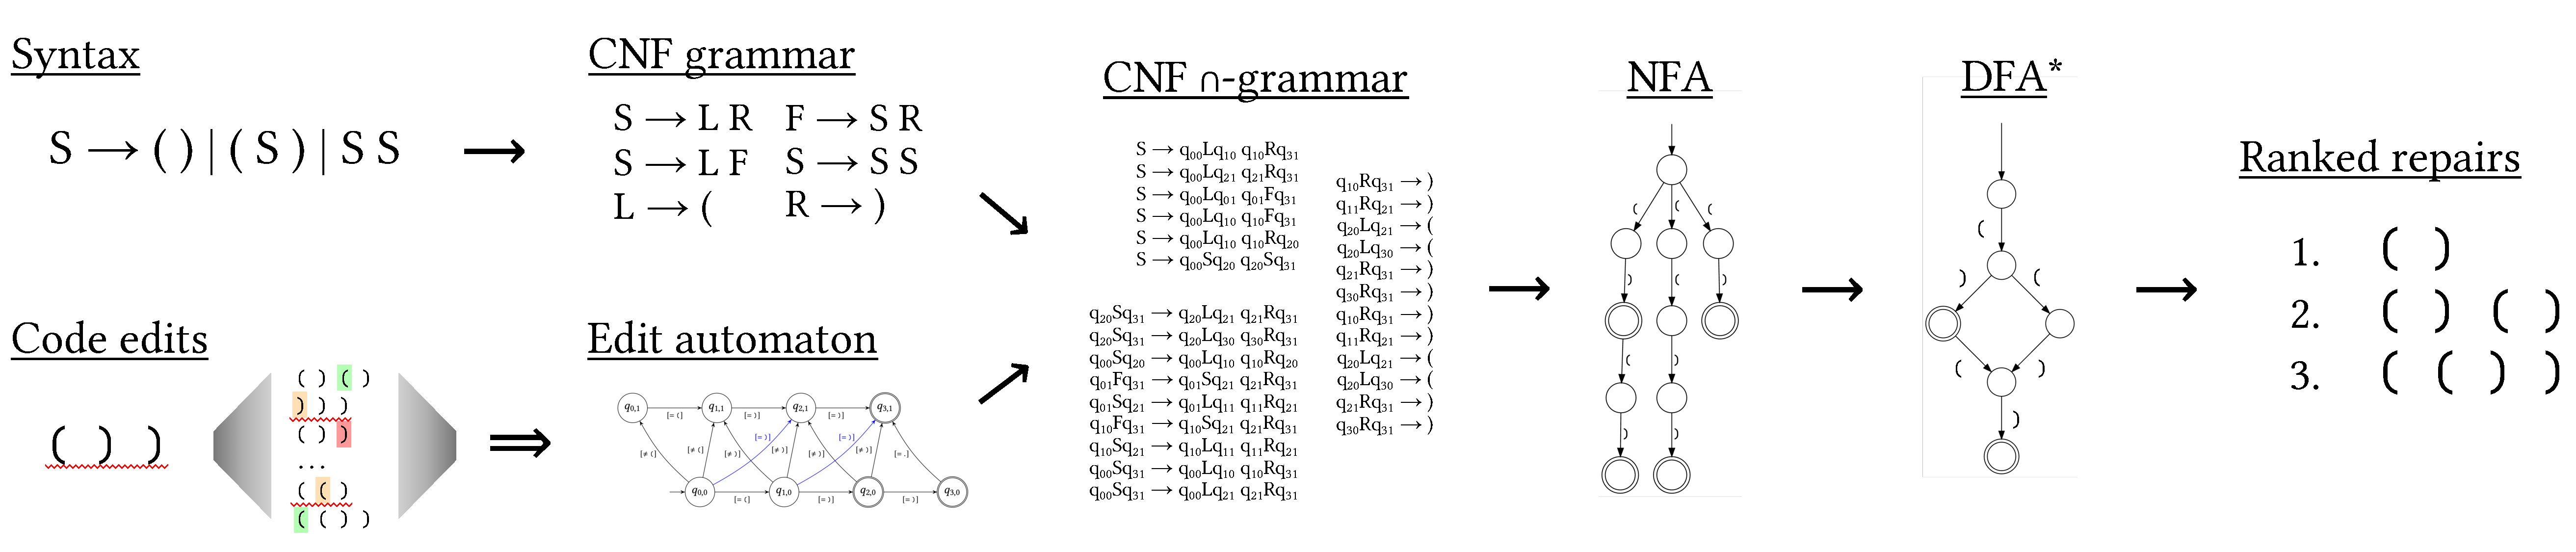
\includegraphics[width=\textwidth]{flow_short}
\vspace{0.1cm}
\caption{Simplified dataflow of the language intersection pipeline. Given a grammar and broken code fragment, we (1) create a automaton generating the language of small edits, then (2) construct a grammar representing the intersection of the two languages. This grammar can be (3) converted into a finite automaton, (4) determinized, then (5) decoded to produce a list of repairs.}
\label{fig:exampleDFA}
\end{figure}
\end{frame}

\section{Formal Language Theory}\label{sec:fltheory}


\section{Algebraic Parsing}\label{sec:algebraic-parsing}

\begin{frame}[fragile]{Parsing for linear algebraists}
  Given a CFG $\mathcal{G} \coloneqq \langle V, \Sigma, P, S\rangle$ in Chomsky Normal Form, we can construct a recognizer $R_\mathcal{G}: \Sigma^n \rightarrow \mathbb{B}$ for strings $\sigma: \Sigma^n$ as follows. Let $2^V$ be our domain, $0$ be $\varnothing$, $\oplus$ be $\cup$, and $\otimes$ be defined as follows:

  \vspace{-7pt}
  \[
    s_1 \otimes s_2 \coloneqq \{C \mid \langle A, B\rangle \in s_1 \times s_2, (C\rightarrow AB) \in P\}\\
    \text{e.g.},
    \{A \rightarrow BC, C \rightarrow AD, D \rightarrow BA\} \subseteq P \vdash \{A, B, C\} \otimes \{B, C, D\} = \{A, C\}
  \]
  \vspace{-1.5cm}

  \noindent If we define $\sigma_r^{\shur} \coloneqq \{w \mid (w \rightarrow \sigma_r) \in P\}$, then initialize $M^0_{r+1=c}(\mathcal{G}', e) := \;\sigma_r^{\shur}$ and solve for the fixpoint $M^* = M + M^2$,\vspace{-10pt}

  \begin{align*}
    M^0:=
    \begin{pNiceMatrix}[xdots/line-style=loosely dotted]
      \varnothing & \sigma_1^\shri & \varnothing & \Cdots & \varnothing \\
      \Vdots      & \Ddots         & \Ddots      & \Ddots & \Vdots\\
                  &                &             &        & \varnothing\\
                  &                &             &        & \sigma_n^\shup \\
      \varnothing & \Cdots         &             &        & \varnothing
    \end{pNiceMatrix} &\Rightarrow \ldots \Rightarrow M^* =
    \begin{pNiceMatrix}[xdots/line-style=loosely dotted]
      \varnothing & \sigma_1^\shri & \Lambda & \Cdots & \Lambda^*_\sigma\\
      \Vdots      & \Ddots         & \Ddots  & \Ddots & \Vdots\\
                  &                &         &        & \Lambda\\
                  &                &         &        & \sigma_n^\shup \\
      \varnothing & \Cdots         &         &        & \varnothing
    \end{pNiceMatrix}
  \end{align*}

  \noindent $S \Rightarrow^* \sigma \iff \sigma \in \mathcal{L}(\mathcal{G})$ iff $S \in \Lambda^*_\sigma$, i.e., $\mathds{1}_{\Lambda^*_\sigma}(S) \iff \mathds{1}_{\mathcal{L}(\mathcal{G})}(\sigma)$.
\end{frame}

\begin{frame}[fragile]{Satisfiability + holes}
  Let us consider an example with two holes, $\sigma = 1$ \hole\phantom{.}\hole, and the grammar being $G\coloneqq\{S\rightarrow N O N, O \rightarrow + \mid \times, N \rightarrow 0 \mid 1\}$. This can be rewritten into CNF as $G'\coloneqq \{S \rightarrow N L, N \rightarrow 0 \mid 1, O \rightarrow \times \mid +, L \rightarrow O N\}$. Using the algebra where $\oplus=\cup$, $X \otimes Z = \big\{\;w \mid \langle x, z\rangle \in X \times Z, (w\rightarrow xz) \in P\;\big\}$, the fixpoint $M' = M + M^2$ can be computed as follows:\\\vspace{10pt}

  \resizebox{\textwidth}{!}{
{\renewcommand{\arraystretch}{1.2}
\noindent\phantom{...}\begin{tabular}{|c|c|c|c|}
  \hline
  & $2^V$ & $\mathbb{Z}_2^{|V|}$ & $\mathbb{Z}_2^{|V|}\rightarrow\mathbb{Z}_2^{|V|}$\\\hline
  $M_0$ & \begin{pmatrix}
  \phantom{V} & \tiny{\{N\}} &         &             \\
              &              & \{N,O\} &             \\
              &              &         & \{N,O\} \\
              &              &         &
  \end{pmatrix} & \begin{pmatrix}
  \phantom{V} & \ws\bs\ws\ws &              &              \\
              &              & \ws\bs\bs\ws &              \\
              &              &              & \ws\bs\bs\ws \\
              &              &              &
  \end{pmatrix} & \begin{pmatrix}
     \phantom{V} & V_{0, 1} &          &          \\
                 &          & V_{1, 2} &          \\
                 &          &          & V_{2, 3} \\
                 &          &          &
  \end{pmatrix} \\\hline
  $M_1$ & \begin{pmatrix}
  \phantom{V} & \tiny{\{N\}} & \varnothing &         \\
              &              & \{N,O\}     & \{L\}   \\
              &              &             & \{N,O\} \\
              &              &             &
  \end{pmatrix} & \begin{pmatrix}
  \phantom{V} & \ws\bs\ws\ws & \ws\ws\ws\ws &              \\
              &              & \ws\bs\bs\ws & \bs\ws\ws\ws \\
              &              &              & \ws\bs\bs\ws \\
              &              &              &
  \end{pmatrix} & \begin{pmatrix}
                   \phantom{V} & V_{0, 1} & V_{0, 2} &          \\
                   &          & V_{1, 2} & V_{1, 3} \\
                   &          &          & V_{2, 3} \\
                   &          &          &
  \end{pmatrix} \\\hline
  $M_\infty$ & \begin{pmatrix}
  \phantom{V} & \tiny{\{N\}} & \varnothing & \{S\}   \\
              &              & \{N,O\}     & \{L\}   \\
              &              &             & \{N,O\} \\
              &              &             &
  \end{pmatrix} & \begin{pmatrix}
  \phantom{V} & \ws\bs\ws\ws & \ws\ws\ws\ws & \ws\ws\ws\bs \\
              &              & \ws\bs\bs\ws & \bs\ws\ws\ws \\
              &              &              & \ws\bs\bs\ws \\
              &              &              &
  \end{pmatrix} & \begin{pmatrix}
                   \phantom{V} & V_{0, 1} & V_{0, 2} & V_{0, 3} \\
                   &          & V_{1, 2} & V_{1, 3} \\
                   &          &          & V_{2, 3} \\
                   &          &          &
  \end{pmatrix}\\\hline
\end{tabular}
}
  }
\end{frame}

%------------------------------------------------------------------------------------------------

\begin{frame}[fragile]{Background: Regular grammars}
  A regular grammar (RG) is a quadruple $\mathcal{G} = \langle V, \Sigma, P, S\rangle$ where $V$ are nonterminals, $\Sigma$ are terminals, $P: V\times (V \cup \Sigma)^{\leq 2}$ are the productions, and $S\in V$ is the start symbol, i.e., all productions are of the form $A \rightarrow a$, $A \rightarrow a B$ (right-regular), or $A \rightarrow B a$ (left-regular). e.g., the following RG and NFA correspond to the language defined by the \textit{regex} \tinline{(a(ab)*)*(ba)*}:

  % https://www3.nd.edu/~kogge/courses/cse30151-fa17/Public/other/tikz_tutorial.pdf
  % Glushkov's algorithm: https://www.irif.fr/~jep/PDF/MPRI/MPRI.pdf#subsection.3.5.2
  \begin{figure}
    \hspace{-1cm}
    \begin{minipage}[t]{0.25\linewidth}
      \vspace{-2.4cm}\scalebox{0.6}{
        \begin{aligned}[t]
          S &\rightarrow Q_0 \mid Q_2 \mid Q_3 \mid Q_5\\
          Q_0 &\rightarrow \varepsilon \\
          Q_1 &\rightarrow Q_0 b \mid Q_2 b\\
          Q_2 &\rightarrow Q_1 a \\
          Q_3 &\rightarrow Q_0 a \mid Q_3 a \mid Q_5 a \\
          Q_4 &\rightarrow Q_3 a \mid Q_5 a \\
          Q_5 &\rightarrow Q_4 b \\
        \end{aligned}}
    \end{minipage}
    \hspace{0.5cm}
    \begin{minipage}[t]{0.48\linewidth}
      \scalebox{0.5}{
        \begin{tikzpicture}
          [->, >=stealth,]
          \node[state, initial above, accepting] (Q0) {$Q_0$};
          \node[state, left of=Q0] (Q1) {$Q_1$};
          \node[state, accepting, left of=Q1] (Q2) {$Q_2$};
          \node[state, accepting, right of=Q0] (Q3) {$Q_3$};
          \node[state, above right of=Q3] (Q4) {$Q_4$};
          \node[state, accepting, below right of=Q3] (Q5) {$Q_5$};
          \draw
          %        (Q0) edge[loop above] (Q0)
          (Q0) edge node{\ttinline b} (Q1)
          (Q0) edge node{\ttinline a} (Q3)
          (Q1) edge[bend right] node{\ttinline a} (Q2)
          (Q2) edge[bend right] node{\ttinline b} (Q1)
          (Q3) edge[loop above] node{\ttinline a} (Q3)
          (Q3) edge node{\ttinline a} (Q4)
          (Q5) edge node{\ttinline a} (Q3)
          (Q4) edge[bend left] node{\ttinline b} (Q5)
          (Q5) edge[bend left] node{\ttinline a} (Q4)
        \end{tikzpicture}
      }
    \end{minipage}
  \end{figure}

  \begin{center}
    \scalebox{0.8}{
      \begin{tikzpicture}[font=\sffamily,breathe dist/.initial=4ex]
        \foreach \X [count=\Y,remember=\Y as \LastY] in
          {finite,regular}
          {\ifnum\Y=1
        \node[ellipse,draw,outer sep=0pt] (F-\Y) {\X};
        \else
        \path[decoration={text along path,
        text={|\sffamily|\X},text align=center,raise=0.9ex},decorate]
        let \p1=($(F-\LastY.north)-(F-\LastY.west)$)
        in (F-\LastY.west) arc(180:0:\x1 and \y1);
        \path let \p1=($([yshift=\pgfkeysvalueof{/tikz/breathe dist}]F-\LastY.north)
        -(F-\LastY.south)$),
        \p2=($(F-1.east)-(F-1.west)$),\p3=($(F-1.north)-(F-1.south)$)
        in ($([yshift=\pgfkeysvalueof{/tikz/breathe dist}]F-\LastY.north)!0.5!(F-\LastY.south)$)
        node[minimum height=\y1,minimum width={\y1*\x2/\y3},
        draw,ellipse,inner sep=0pt, fill=black!30!white] (F-\Y){};
        \fi
        }
        \foreach \X [count=\Y,remember=\Y as \LastY] in
          {finite,regular,context-free}
          {\ifnum\Y=1
        \node[ellipse,draw,outer sep=0pt] (F-\Y) {\X};
        \else
        \path[decoration={text along path,
        text={|\sffamily|\X},text align=center,raise=0.9ex},decorate]
        let \p1=($(F-\LastY.north)-(F-\LastY.west)$)
        in (F-\LastY.west) arc(180:0:\x1 and \y1);
        \path let \p1=($([yshift=\pgfkeysvalueof{/tikz/breathe dist}]F-\LastY.north)
        -(F-\LastY.south)$),
        \p2=($(F-1.east)-(F-1.west)$),\p3=($(F-1.north)-(F-1.south)$)
        in ($([yshift=\pgfkeysvalueof{/tikz/breathe dist}]F-\LastY.north)!0.5!(F-\LastY.south)$)
        node[minimum height=\y1,minimum width={\y1*\x2/\y3},
        draw,ellipse,inner sep=0pt] (F-\Y){};
        \fi}
      \end{tikzpicture}
    }
  \end{center}
\end{frame}

    \begin{frame}[fragile]{Levenshtein automaton customization}

Consider the string $\err\sigma=$ \texttt{\scriptsize ( ) )} and the alphabet $\Sigma = \{\texttt{\scriptsize)}, \texttt{\scriptsize(}\}$. Every string within one edit of $\err\sigma$ is recognized by an NFA with the following structure:

\begin{figure}[h!]
\resizebox{0.45\textwidth}{!}{
\begin{tikzpicture}[
%->, % makes the edges directed
>=stealth',
node distance=2.5cm, % specifies the minimum distance between two nodes. Change if necessary.
%  every state/.style={thick, fill=gray!10}, % sets the properties for each ’state’ node
initial text=$ $, % sets the text that appears on the start arrow
]
\node[state, initial]                (00) {$q_{0,0}$};
\node[state, right of=00]            (10) {$q_{1,0}$};
\node[accepting, state, right of=10] (20) {$q_{2,0}$};
\node[accepting, state, right of=20] (30) {$q_{3,0}$};

\node[state, above of=00, shift={(-2cm,0cm)}] (01) {$q_{0,1}$};
\node[state, right of=01]                     (11) {$q_{1,1}$};
\node[state, right of=11]                     (21) {$q_{2,1}$};
\node[accepting, state, right of=21]          (31) {$q_{3,1}$};

\draw [->] (00) edge[below] node{$\texttt{(}$} (10);
\draw [->] (10) edge[below] node{$\texttt{)}$} (20);
\draw [->] (20) edge[below] node{$\texttt{)}$} (30);

\draw [->] (01) edge[below] node{$\texttt{(}$}                       (11);
\draw [->] (11) edge[below] node[shift={(-0.2cm,0cm)}]{$\texttt{)}$} (21);
\draw [->] (21) edge[below] node[shift={(-0.2cm,0cm)}]{$\texttt{)}$} (31);

\draw [->] (00) edge[bend left=10] node[shift={(-0.15cm,0cm)}]{\tiny{$\texttt{(}$}} (11);
\draw [->] (10) edge[bend left=10] node[shift={(-0.15cm,0cm)}]{\tiny{$\texttt{(}$}} (21);
\draw [->] (20) edge[bend left=10] node[shift={(-0.15cm,0cm)}]{\tiny{$\texttt{(}$}} (31);

\draw [->] (00) edge[bend left=10, left] node[shift={(-0.1cm,0cm)}]{\tiny{$\texttt{(}$}} (01);
\draw [->] (10) edge[bend left=10, left] node[shift={(-0.1cm,0cm)}]{\tiny{$\texttt{(}$}} (11);
\draw [->] (20) edge[bend left=10, left] node[shift={(-0.1cm,0cm)}]{\tiny{$\texttt{(}$}} (21);

\draw [->] (00) edge[bend right=10, right] node{\tiny{$\texttt{)}$}} (11);
\draw [->] (10) edge[bend right=10, right] node{\tiny{$\texttt{)}$}} (21);
\draw [->] (20) edge[bend right=10, right] node{\tiny{$\texttt{)}$}} (31);

\draw [->] (00) edge[bend right=10, right] node{\tiny{$\texttt{)}$}} (01);
\draw [->] (10) edge[bend right=10, right] node{\tiny{$\texttt{)}$}} (11);
\draw [->] (20) edge[bend right=10, right] node{\tiny{$\texttt{)}$}} (21);

\draw [->] (30) edge[bend left=10, left] node[shift={(-0.1cm,0cm)}]{\tiny{$\texttt{(}$}} (31);
\draw [->] (30) edge[bend right=10, right] node{\tiny{$\texttt{)}$}} (31);

\draw [->, blue] (00) edge[bend right=11,below] node[shift={(0.4cm,0.9cm)}]{$\texttt{)}$}    (21);
\draw [->, blue] (10) edge[bend right=11,below] node[shift={(0.4cm,0.9cm)}]{$\texttt{)}$}    (31);
\node[align=center, yshift=2em, xshift=-1cm] (title) at (current bounding box.north) {Original Levenshtein automaton};
\end{tikzpicture}
}
\resizebox{0.515\textwidth}{!}{
\begin{tikzpicture}[
%->, % makes the edges directed
>=stealth',
node distance=2.5cm, % specifies the minimum distance between two nodes. Change if necessary.
%  every state/.style={thick, fill=gray!10}, % sets the properties for each ’state’ node
initial text=$ $, % sets the text that appears on the start arrow
]
\draw[orange,->] (-4cm,1.2cm) -- (-3cm,1.2cm);

\node[state, initial]                (00) {$q_{0,0}$};
\node[state, right of=00]            (10) {$q_{1,0}$};
\node[accepting, state, right of=10] (20) {$q_{2,0}$};
\node[accepting, state, right of=20] (30) {$q_{3,0}$};

\node[state, above of=00, shift={(-2cm,0cm)}] (01) {$q_{0,1}$};
\node[state, right of=01]                     (11) {$q_{1,1}$};
\node[state, right of=11]                     (21) {$q_{2,1}$};
\node[accepting, state, right of=21]          (31) {$q_{3,1}$};

\draw [->] (00) edge[below] node{\tiny{$[= \texttt{(}]$}} (10);
\draw [->] (10) edge[below] node{\tiny{$[= \texttt{)}]$}} (20);
\draw [->] (20) edge[below] node{\tiny{$[= \texttt{)}]$}} (30);

\draw [->] (01) edge[below] node{\tiny{$[= \texttt{(}]$}}                       (11);
\draw [->] (11) edge[below] node[shift={(-0.2cm,0cm)}]{\tiny{$[= \texttt{)}]$}} (21);
\draw [->] (21) edge[below] node[shift={(-0.2cm,0cm)}]{\tiny{$[= \texttt{)}]$}} (31);

\draw [->] (00) edge[left] node{\tiny{$[\neq \texttt{(}]$}} (11);
\draw [->] (10) edge[left] node{\tiny{$[\neq \texttt{)}]$}} (21);
\draw [->] (20) edge[left] node{\tiny{$[\neq \texttt{)}]$}} (31);

\draw [->] (00) edge[bend left=10, left] node{\tiny{$[\neq \texttt{(}]$}} (01);
\draw [->] (10) edge[bend left=10, left] node{\tiny{$[\neq \texttt{)}]$}} (11);
\draw [->] (20) edge[bend left=10, left] node{\tiny{$[\neq \texttt{)}]$}} (21);
\draw [->] (30) edge[bend left=10, left] node{\tiny{$[=.]$}} (31);


\draw [->, blue] (00) edge[bend right=11,below] node[shift={(0.2cm,0.8cm)}]{\tiny{$[= \texttt{)}]$}}    (21);
\draw [->, blue] (10) edge[bend right=11,below] node[shift={(0.2cm,0.8cm)}]{\tiny{$[= \texttt{)}]$}}    (31);
\node[align=center, yshift=2em, xshift=-0.4cm] (title) at (current bounding box.north) {Nominal Levenshtein automaton (ours)};
\end{tikzpicture}
}
\caption{Automaton recognizing every single patch of the broken string \texttt{( ) )} within Levenshtein distance 1. We nominalize the original Levenshtein automaton, ensuring upward arcs denote a mutation, and replace terminals with a symbolic predicate, which deduplicates parallel arcs in large alphabets.}\label{fig:lev_automaton}\vspace{-5pt}
\end{figure}
\\
\tiny{\url{https://fulmicoton.com/posts/levenshtein/#observations-lets-count-states}}
\end{frame}

\begin{frame}[fragile]{Levenshtein reachability}
  \begin{figure}[H]
    \resizebox{\textwidth}{!}{
      \begin{tikzpicture}[
%->, % makes the edges directed
        >=stealth',
        node distance=2.5cm, % specifies the minimum distance between two nodes. Change if necessary.
%  every state/.style={thick, fill=gray!10}, % sets the properties for each ’state’ node
        initial text=$ $, % sets the text that appears on the start arrow
      ]
        \node[state, initial]                (00) {$q_{0,0}$};
        \node[state, right of=00]            (10) {$q_{1,0}$};
        \node[accepting, state, right of=10] (20) {$q_{2,0}$};
        \node[accepting, state, right of=20] (30) {$q_{3,0}$};
        \node[accepting, state, right of=30] (40) {$q_{4,0}$};
        \node[accepting, state, right of=40] (50) {$q_{5,0}$};

        \node[state, above of=00, shift={(-2cm,0cm)}] (01) {$q_{0,1}$};
        \node[state, right of=01]                          (11) {$q_{1,1}$};
        \node[state, right of=11]                          (21) {$q_{2,1}$};
        \node[accepting, state, right of=21]               (31) {$q_{3,1}$};
        \node[accepting, state, right of=31]               (41) {$q_{4,1}$};
        \node[accepting, state, right of=41]               (51) {$q_{5,1}$};

        \node[state, above of=01, shift={(-2cm,0cm)}] (0j) {$q_{0,2}$};
        \node[state, right of=0j]                          (1j) {$q_{1,2}$};
        \node[state, right of=1j]                          (2j) {$q_{2,2}$};
        \node[state, right of=2j]                          (3j) {$q_{3,2}$};
        \node[accepting, state, right of=3j]               (4j) {$q_{4,2}$};
        \node[accepting, state, right of=4j]               (5j) {$q_{5,2}$};

        \node[state, above of=0j, shift={(-2cm,0cm)}] (0k) {$q_{0,3}$};
        \node[state, right of=0k]                         (1k) {$q_{1,3}$};
        \node[state, right of=1k]                         (2k) {$q_{2,3}$};
        \node[state, right of=2k]                         (3k) {$q_{3,3}$};
        \node[state, right of=3k]                         (4k) {$q_{4,3}$};
        \node[accepting, state, right of=4k]              (5k) {$q_{5,3}$};

        \draw [->] (00) edge[below] node{$\sigma_1$} (10);
        \draw [->] (10) edge[below] node{$\sigma_2$} (20);
        \draw [->] (20) edge[below] node{$\sigma_3$} (30);
        \draw [->] (30) edge[below] node{$\sigma_4$} (40);
        \draw [->] (40) edge[below] node{$\sigma_5$} (50);

        \draw [->] (01) edge[below] node{$\sigma_1$} (11);
        \draw [->] (11) edge[below] node[shift={(-0.2cm,0cm)}]{$\sigma_2$} (21);
        \draw [->] (21) edge[below] node[shift={(-0.2cm,0cm)}]{$\sigma_3$} (31);
        \draw [->] (31) edge[below] node[shift={(-0.2cm,0cm)}]{$\sigma_4$} (41);
        \draw [->] (41) edge[below] node{$\sigma_5$} (51);

        \draw [->] (0j) edge[below] node{$\sigma_1$} (1j);
        \draw [->] (1j) edge[below] node{$\sigma_2$} (2j);
        \draw [->] (2j) edge[below] node{$\sigma_3$} (3j);
        \draw [->] (3j) edge[below] node{$\sigma_4$} (4j);
        \draw [->] (4j) edge[below] node{$\sigma_5$} (5j);

        \draw [->] (0k) edge[below] node{$\sigma_1$} (1k);
        \draw [->] (1k) edge[below] node{$\sigma_2$} (2k);
        \draw [->] (2k) edge[below] node{$\sigma_3$} (3k);
        \draw [->] (3k) edge[below] node{$\sigma_4$} (4k);
        \draw [->] (4k) edge[below] node{$\sigma_5$} (5k);

        \draw [->] (00) edge[left] node{$\phantom{\cdot}$} (11);
        \draw [->] (10) edge[left] node{$\phantom{\cdot}$} (21);
        \draw [->] (20) edge[left] node{$\phantom{\cdot}$} (31);
        \draw [->] (30) edge[left] node{$\phantom{\cdot}$} (41);
        \draw [->] (40) edge[left] node{$\phantom{\cdot}$} (51);

% Super-knight arcs
        \draw [->, red] (00) edge[bend right=8] node[east, shift={(-0.2cm,-0.7cm)}]{$\color{red}\sigma_3$}         (3j);
        \draw [->, red] (10) edge[bend right=8] node[east, shift={(-0.2cm,-0.7cm)}]{$\color{red}\sigma_4$}         (4j);
        \draw [->, red] (20) edge[bend right=8] node[east, shift={(-0.2cm,-0.7cm)}]{$\color{red}\sigma_5$}         (5j);

        \draw [->, red] (01) edge[bend left=8] node[east, shift={(-0.2cm,-0.7cm)}]{$\color{red}\sigma_3$}         (3k);
        \draw [->, red] (11) edge[bend left=8] node[east, shift={(-0.2cm,-0.7cm)}]{$\color{red}\sigma_4$}         (4k);
        \draw [->, red] (21) edge[bend left=8] node[east, shift={(-0.2cm,-0.7cm)}]{$\color{red}\sigma_5$}         (5k);

        \draw [->, violet] (00) edge node[east, shift={(-0.1cm,-0.8cm)}]{$\color{violet}\sigma_4$}  (4k);
        \draw [->, violet] (10) edge node[east, shift={(-0.1cm,-0.8cm)}]{$\color{violet}\sigma_5$}  (5k);

        \draw [->] (01) edge[left] node{$\phantom{\cdot}$} (1j);
        \draw [->] (11) edge[left] node{$\phantom{\cdot}$} (2j);
        \draw [->] (21) edge[left] node{$\phantom{\cdot}$} (3j);
        \draw [->] (31) edge[left] node{$\phantom{\cdot}$} (4j);
        \draw [->] (41) edge[left] node{$\phantom{\cdot}$} (5j);

        \draw [->] (0j) edge[left] node{$\phantom{\cdot}$} (1k);
        \draw [->] (1j) edge[left] node{$\phantom{\cdot}$} (2k);
        \draw [->] (2j) edge[left] node{$\phantom{\cdot}$} (3k);
        \draw [->] (3j) edge[left] node{$\phantom{\cdot}$} (4k);
        \draw [->] (4j) edge[left] node{$\phantom{\cdot}$} (5k);

        \draw [->] (00) edge[bend left=10, left] node{$\phantom{\cdot}$} (01);
        \draw [->] (10) edge[bend left=10, left] node{$\phantom{\cdot}$} (11);
        \draw [->] (20) edge[bend left=10, left] node{$\phantom{\cdot}$} (21);
        \draw [->] (30) edge[bend left=10, left] node{$\phantom{\cdot}$} (31);
        \draw [->] (40) edge[bend left=10, left] node{$\phantom{\cdot}$} (41);
        \draw [->] (50) edge[bend left=10, left] node{$\phantom{\cdot}$} (51);

        \draw [->] (01) edge[bend left=10, left] node{$\phantom{\cdot}$} (0j);
        \draw [->] (11) edge[bend left=10, left] node{$\phantom{\cdot}$} (1j);
        \draw [->] (21) edge[bend left=10, left] node{$\phantom{\cdot}$} (2j);
        \draw [->] (31) edge[bend left=10, left] node{$\phantom{\cdot}$} (3j);
        \draw [->] (41) edge[bend left=10, left] node{$\phantom{\cdot}$} (4j);
        \draw [->] (51) edge[bend left=10, left] node{$\phantom{\cdot}$} (5j);

        \draw [->] (0j) edge[bend left=10, left] node{$\phantom{\cdot}$} (0k);
        \draw [->] (1j) edge[bend left=10, left] node{$\phantom{\cdot}$} (1k);
        \draw [->] (2j) edge[bend left=10, left] node{$\phantom{\cdot}$} (2k);
        \draw [->] (3j) edge[bend left=10, left] node{$\phantom{\cdot}$} (3k);
        \draw [->] (4j) edge[bend left=10, left] node{$\phantom{\cdot}$} (4k);
        \draw [->] (5j) edge[bend left=10, left] node{$\phantom{\cdot}$} (5k);

        \draw [->, blue] (00) edge[bend right=11,below] node[shift={(0.5cm,0.3cm)}]{$\color{blue}\sigma_2$}    (21);
        \draw [->, blue] (10) edge[bend right=11,below] node[shift={(0.5cm,0.3cm)}]{$\color{blue}\sigma_3$}    (31);
        \draw [->, blue] (20) edge[bend right=11,below] node[shift={(0.5cm,0.3cm)}]{$\color{blue}\sigma_4$}    (41);
        \draw [->, blue] (30) edge[bend right=11,below] node[shift={(0.5cm,0.3cm)}]{$\color{blue}\sigma_5$}    (51);

        \draw [->, blue] (01) edge[bend right=3,below] node[shift={(0.3cm,0.2cm)}]{$\color{blue}\sigma_2$}    (2j);
        \draw [->, blue] (11) edge[bend right=3,below] node[shift={(0.3cm,0.2cm)}]{$\color{blue}\sigma_3$}    (3j);
        \draw [->, blue] (21) edge[bend right=3,below] node[shift={(0.3cm,0.2cm)}]{$\color{blue}\sigma_4$}    (4j);
        \draw [->, blue] (31) edge[bend right=3,below] node[shift={(0.3cm,0.2cm)}]{$\color{blue}\sigma_4$}    (5j);

        \draw [->, blue] (0j) edge[bend left=8,below] node[shift={(-0.45cm,-0.55cm)}]{$\color{blue}\sigma_2$}    (2k);
        \draw [->, blue] (1j) edge[bend left=8,below] node[shift={(-0.45cm,-0.55cm)}]{$\color{blue}\sigma_3$}    (3k);
        \draw [->, blue] (2j) edge[bend left=8,below] node[shift={(-0.45cm,-0.55cm)}]{$\color{blue}\sigma_4$}    (4k);
        \draw [->, blue] (3j) edge[bend left=8,below] node[shift={(-0.45cm,-0.55cm)}]{$\color{blue}\sigma_5$}    (5k);

%https://tex.stackexchange.com/a/20986/139648
        \draw [decorate,decoration={brace,amplitude=10pt,raise=10pt,mirror}] (00.south west) -- (50.south east) node[midway,yshift=-3em]{\textbf{String length}};
        \draw [decorate,decoration={brace,amplitude=10pt,raise=20pt}] (00.south west) -- (0k.north west) node[midway,xshift=-1cm,yshift=-1cm,rotate=-54]{\textbf{Edit distance}};
      \end{tikzpicture}
    }
    \caption{Bounded Levenshtein reachability from $\sigma: \Sigma^n$ is expressible as an NFA populated by accept states within radius $k$ of $S=q_{n,0}$, which accepts all strings $\sigma'$ within Levenshtein radius $k$ of $\sigma$.}
  \end{figure}
\end{frame}

\begin{frame}[fragile]{The nominal Levenshtein automaton}
  The original Levenshtein automaton (Schulz \& Stoyan, 2002):

  \begin{prooftree}
    \AxiomC{$s\in\Sigma \phantom{\land} i \in [0, n] \phantom{\land} j \in [1, k]$}
    \RightLabel{$\duparrow$}
    \UnaryInfC{$(q_{i, j-1} \overset{s}{\rightarrow} q_{i,j}) \in \delta$}
    \DisplayProof
    \hskip 1.5em
    \AxiomC{$s\in\Sigma \phantom{\land} i \in [1, n] \phantom{\land} j \in [1, k]$}
    \RightLabel{$\ddiagarrow$}
    \UnaryInfC{$(q_{i-1, j-1} \overset{s}{\rightarrow} q_{i,j}) \in \delta$}
  \end{prooftree}
  \begin{prooftree}
    \AxiomC{$s=\sigma_i \phantom{\land} i \in [1, n] \phantom{\land} j \in [0, k]$}
    \RightLabel{$\drightarrow$}
    \UnaryInfC{$(q_{i-1, j} \overset{s}{\rightarrow} q_{i,j}) \in \delta$}
    \DisplayProof
    \hskip 1.5em
    \AxiomC{$s=\sigma_i \phantom{\land} i \in [2, n] \phantom{\land} j \in [1, k]$}
    \RightLabel{$\knightarrow$}
    \UnaryInfC{$(q_{i-2, j-1} \overset{s}{\rightarrow} q_{i,j}) \in \delta$}
  \end{prooftree}
  \begin{prooftree}
    \AxiomC{$\vphantom{|}$}
    \RightLabel{$\textsc{Init}$}
    \UnaryInfC{$q_{0,0} \in I$}
    \DisplayProof
    \hskip 1.5em
    \AxiomC{$q_{i, j}$}
    \AxiomC{$|n-i+j| \leq k$}
    \RightLabel{$\textsc{Done}$}
    \BinaryInfC{$q_{i, j}\in F$}
  \end{prooftree}

  We modify the original automaton with a nominal predicate:

  \begin{prooftree}
    \AxiomC{$i \in [0, n] \phantom{\land} j \in [1, k]$}
    \RightLabel{$\duparrow$}
    \UnaryInfC{$(q_{i, j-1} \overset{{\color{orange}[\neq \sigma_{i+1}]}}{\rightarrow} q_{i,j}) \in \delta$}
    \DisplayProof
    \hskip 1.5em
    \AxiomC{$i \in [1, n] \phantom{\land} j \in [1, k]$}
    \RightLabel{$\ddiagarrow$}
    \UnaryInfC{$(q_{i-1, j-1} \overset{{\color{orange}[\neq \sigma_i]}}{\rightarrow} q_{i,j}) \in \delta$}
  \end{prooftree}
  \begin{prooftree}
    \AxiomC{$i \in [1, n] \phantom{\land} j \in [0, k]$}
    \RightLabel{$\drightarrow$}
    \UnaryInfC{$(q_{i-1, j} \overset{{\color{orange}[=\sigma_i]}}{\rightarrow} q_{i,j}) \in \delta$}
    \DisplayProof
    \hskip 1.5em
    \AxiomC{$d \in [1, d_{\max}] \phantom{\land} i \in [d + 1, n] \phantom{\land} j \in [d, k]$}
    \RightLabel{$\knightarrow$}
    \UnaryInfC{$(q_{i-d-1, j-d} \overset{{\color{orange}[=\sigma_i]}}{\rightarrow} q_{i,j}) \in \delta$}
  \end{prooftree}
\end{frame}

\begin{frame}[fragile]{Geometrically interpreting the edit calculus}

Each arc plays a specific role. $\duparrow$ handles insertions, $\ddiagarrow$ handles substitutions and $\knightarrow$ handles deletions of $\geq 1$ tokens. Consider some illustrative cases:

\vspace{0.5cm}

\newcommand{\substitutionExample}{
\tikz{
\foreach \x in {0,8,16,24,32,40}{
\fill (\x pt,0pt) circle [radius = 1pt];
\fill (\x pt,8pt) circle [radius = 1pt];
}
\phantom{\fill (0pt,-8pt) circle [radius = 1pt];}
\draw [-to] (0pt,0pt) -- (8pt,0pt);
\draw [-to] (8pt,0pt) -- (16pt,0pt);
\draw [-to] (16pt,0pt) -- (24pt,8pt);
\draw [-to] (24pt,8pt) -- (32pt,8pt);
\draw [-to] (32pt,8pt) -- (40pt,8pt);
}
}

\newcommand{\insertionExample}{
\tikz{
\foreach \x in {0,8,16,24,32,40}{
\fill (\x pt,0pt) circle [radius = 1pt];
\fill (\x pt,8pt) circle [radius = 1pt];
}
\phantom{\fill (0pt,-8pt) circle [radius = 1pt];}
\fill[white] (16pt,0pt) circle [radius = 1.2pt];
\fill[white] (24pt,8pt) circle [radius = 1.2pt];
\draw [-to] (0pt,0pt) -- (8pt,0pt);
\draw [-to] (8pt,0pt) -- (24pt,0pt);
\draw [-to] (24pt,0pt) -- (16pt,8pt);
\draw [-to] (16pt,8pt) -- (32pt,8pt);
\draw [-to] (32pt,8pt) -- (40pt,8pt);
}
}

\newcommand{\deletionExample}{
\tikz{
\foreach \x in {0,8,16,24,32,40}{
\fill (\x pt,0pt) circle [radius = 1pt];
\fill (\x pt,8pt) circle [radius = 1pt];
}
\phantom{\fill (0pt,-8pt) circle [radius = 1pt];}
\draw [-to] (0pt,0pt) -- (8pt,0pt);
\draw [-to] (8pt,0pt) -- (16pt,0pt);
\draw [-to] (16pt,0pt) -- (24pt,0pt);
\draw [-to] (24pt,0pt) -- (40pt,8pt);
}
}

\newcommand{\doubleDeletionExample}{
\tikz{
\foreach \x in {0,8,16,24,32,40}{
\fill (\x pt,0pt) circle [radius = 1pt];
\fill (\x pt,8pt) circle [radius = 1pt];
\fill (\x pt,16pt) circle [radius = 1pt];
}
\draw [-to] (0pt,0pt) -- (24pt,16pt);
\draw [-to] (24pt,16pt) -- (32pt,16pt);
\draw [-to] (32pt,16pt) -- (40pt,16pt);
}
}

\newcommand{\subDelExample}{
\tikz{
\foreach \x in {0,8,16,24,32,40}{
\fill (\x pt,0pt) circle [radius = 1pt];
\fill (\x pt,8pt) circle [radius = 1pt];
\fill (\x pt,16pt) circle [radius = 1pt];
}
\draw [-to] (0pt,0pt) -- (8pt,0pt);
\draw [-to] (8pt,0pt) -- (16pt,8pt);
\draw [-to] (16pt,8pt) -- (32pt,16pt);
\draw [-to] (32pt,16pt) -- (40pt,16pt);
}
}

\newcommand{\subSubExample}{
\tikz{
\foreach \x in {0,8,16,24,32,40}{
\fill (\x pt,0pt) circle [radius = 1pt];
\fill (\x pt,8pt) circle [radius = 1pt];
\fill (\x pt,16pt) circle [radius = 1pt];
}
\draw [-to] (0pt,0pt) -- (8pt,0pt);
\draw [-to] (8pt,0pt) -- (16pt,8pt);
\draw [-to] (16pt,8pt) -- (24pt,16pt);
\draw [-to] (24pt,16pt) -- (32pt,16pt);
\draw [-to] (32pt,16pt) -- (40pt,16pt);
}
}

\newcommand{\insertDeleteExample}{
\tikz{
\foreach \x in {0,8,16,24,32,40,48}{
\fill (\x pt,0pt) circle [radius = 1pt];
\fill (\x pt,8pt) circle [radius = 1pt];
\fill (\x pt,16pt) circle [radius = 1pt];
}
\fill[white] (16pt,16pt) circle [radius = 1.2pt];
\fill[white] (8pt,0pt) circle [radius = 1.2pt];
\fill[white] (16pt,8pt) circle [radius = 1.2pt];
\draw [-to] (0pt,0pt) -- (16pt,0pt);
\draw [-to] (16pt,0pt) -- (8pt,8pt);
\draw [-to] (8pt,8pt) -- (24pt,8pt);
\draw [-to] (24pt,8pt) -- (40pt,16pt);
\draw [-to] (40pt,16pt) -- (48pt,16pt);
}
}

\footnotesize{
\begin{table}[h!]
\begin{tabular}{ccccc}

\texttt{f\hspace{3pt}.\hspace{3pt}\hlorange{[}\hspace{3pt}x\hspace{3pt})} &
\texttt{f\hspace{3pt}.\hspace{3pt}\phantom{(}\hspace{3pt}x\hspace{3pt})} &
\texttt{f\hspace{3pt}.\hspace{3pt}(\hspace{3pt}\hlred{x}\hspace{3pt})} &
\texttt{\hlred{.}\hspace{3pt}\hlred{+}\hspace{3pt}(\hspace{3pt}x\hspace{3pt})} &
\texttt{f\hspace{3pt}\hlorange{.}\hspace{3pt}\hlred{(}\hspace{3pt}x\hspace{3pt};} \\

\texttt{f\hspace{3pt}.\hspace{3pt}\hlorange{(}\hspace{3pt}x\hspace{3pt})} &
\texttt{f\hspace{3pt}.\hspace{3pt}\hlgreen{(}\hspace{3pt}x\hspace{3pt})} &
\texttt{f\hspace{3pt}.\hspace{3pt}(\hspace{3pt}\phantom{x}\hspace{3pt})} &
\texttt{\phantom{f}\hspace{3pt}\phantom{.}\hspace{3pt}(\hspace{3pt}x\hspace{3pt})} &
\texttt{f\hspace{3pt}\hlorange{*}\hspace{3pt}\phantom{(}\hspace{3pt}x\hspace{3pt};} \\

\substitutionExample & \insertionExample & \deletionExample & \doubleDeletionExample & \subDelExample
\end{tabular}
\end{table}
}

\normalsize{Note that the same $\langle\err\sigma, \sigma'\rangle$ pair can have multiple Levenshtein alignments:}
\vspace{0.5cm}

\footnotesize{
\begin{table}[h!]
\begin{tabular}{cc}

\texttt{[\hspace{3pt}\hlorange{,}\hspace{3pt}\hlorange{x}\hspace{3pt}y\hspace{3pt}]} &
\texttt{[\hspace{3pt}\phantom{,}\hspace{3pt},\hspace{3pt}\hlred{x}\hspace{3pt}y\hspace{3pt}]} \\

\texttt{[\hspace{3pt}\hlorange{x}\hspace{3pt}\hlorange{,}\hspace{3pt}y\hspace{3pt}]} &
\texttt{[\hspace{3pt}\hlgreen{x}\hspace{3pt},\hspace{3pt}\phantom{x}\hspace{3pt}y\hspace{3pt}]} \\

\subSubExample & \insertDeleteExample
\end{tabular}
\end{table}
}

\normalsize{Non-uniqueness of geodesics has implications for CFG $\cap$ L-NFA ambiguity.}
\end{frame}

\begin{frame}{Background: Context-free grammars}
  In a context-free grammar $\mathcal{G} = \langle V, \Sigma, P, S\rangle$ all productions are of the form $P: V\times (V \cup \Sigma)^+$, i.e., RHS may contain any number of nonterminals, $V$. Recognition decidable in $\mathcal{O}(n^\omega)$, n.b. CFLs are \textbf{not} closed under $\cap$!\newline\\
  %
  For example, consider the grammar $\underline{S \rightarrow S S \mid ( S ) \mid ()}$. This represents the language of balanced parentheses, e.g. $(), ()(), (()), ()(()), (()()), (())()\ldots$\newline\\
  %
  Every CFG has a normal form $P^*: V \times (V^2 \mid \Sigma)$, i.e., every production can be refactored into either $v_0 \rightarrow v_1 v_2$ or $v_0 \rightarrow \sigma$, where $v_{0\ldots2}: V$ and $\sigma: \Sigma$, e.g., $\{S \rightarrow S S \mid ( S ) \mid ()\}\Leftrightarrow^*\{S\rightarrow XR \mid SS \mid LR, L \rightarrow (, R \rightarrow ), X\rightarrow LS\}$

  \begin{center}
    \scalebox{0.8}{
      \begin{tikzpicture}[font=\sffamily,breathe dist/.initial=4ex]
        \foreach \X [count=\Y,remember=\Y as \LastY] in
          {finite,regular,context-free}
          {\ifnum\Y=1
        \node[ellipse,draw,outer sep=0pt] (F-\Y) {\X};
        \else
        \path[decoration={text along path,
        text={|\sffamily|\X},text align=center,raise=0.9ex},decorate]
        let \p1=($(F-\LastY.north)-(F-\LastY.west)$)
        in (F-\LastY.west) arc(180:0:\x1 and \y1);
        \path let \p1=($([yshift=\pgfkeysvalueof{/tikz/breathe dist}]F-\LastY.north)
        -(F-\LastY.south)$),
        \p2=($(F-1.east)-(F-1.west)$),\p3=($(F-1.north)-(F-1.south)$)
        in ($([yshift=\pgfkeysvalueof{/tikz/breathe dist}]F-\LastY.north)!0.5!(F-\LastY.south)$)
        node[minimum height=\y1,minimum width={\y1*\x2/\y3},
        draw,ellipse,inner sep=0pt, fill=black!30!white] (F-\Y){};
        \fi
        }
        \foreach \X [count=\Y,remember=\Y as \LastY] in
          {finite,regular,context-free,conjunctive}
          {\ifnum\Y=1
        \node[ellipse,draw,outer sep=0pt] (F-\Y) {\X};
        \else
        \path[decoration={text along path,
        text={|\sffamily|\X},text align=center,raise=0.9ex},decorate]
        let \p1=($(F-\LastY.north)-(F-\LastY.west)$)
        in (F-\LastY.west) arc(180:0:\x1 and \y1);
        \path let \p1=($([yshift=\pgfkeysvalueof{/tikz/breathe dist}]F-\LastY.north)
        -(F-\LastY.south)$),
        \p2=($(F-1.east)-(F-1.west)$),\p3=($(F-1.north)-(F-1.south)$)
        in ($([yshift=\pgfkeysvalueof{/tikz/breathe dist}]F-\LastY.north)!0.5!(F-\LastY.south)$)
        node[minimum height=\y1,minimum width={\y1*\x2/\y3},
        draw,ellipse,inner sep=0pt] (F-\Y){};
        \fi}
      \end{tikzpicture}
    }
  \end{center}
\end{frame}

\begin{frame}[fragile]{Background: Closure properties of formal languages}
  Formal languages are not always closed under set-theoretic operations, e.g., CFL $\cap$ CFL is not CFL in general. Let $\cdot$ denote concatenation, $*$ be Kleene star, and $\complement$ be complementation:\\
  \begin{table}
    \begin{tabular}{c|ccccc}
      & $\cup$ & $\cap$ & $\cdot$ & $*$ & $\complement$ \\\hline
      Finite$^1$                                  & \cmark & \cmark     & \cmark  & \cmark  & \cmark \\
      Regular$^1$                                 & \cmark & \cmark     & \cmark  & \cmark  & \cmark \\
      \rowcolor{slightgray} Context-free$^{1, 2}$ & \cmark & \xmark$^\dagger$ & \cmark  & \cmark  & \xmark \\
      Conjunctive$^{1,2}$                         & \cmark & \cmark     & \cmark  & \cmark  & ?      \\
      Context-sensitive$^2$                       & \cmark & \cmark     & \cmark  & +       & \cmark \\
      Recursively Enumerable$^2$                  & \cmark & \cmark     & \cmark  & \cmark  & \xmark \\
    \end{tabular}
  \end{table}
  We would like a language family that is (1) tractable, i.e., has polynomial recognition and search complexity and (2) reasonably expressive, i.e., can represent syntactic properties of real-world programming languages.\vspace{0.2cm}

  $^\dagger$ However, CFLs are closed under intersection with regular languages.
\end{frame}


\begin{frame}[t,fragile]{The Bar-Hillel construction and its specialization}
  \begin{theorem}[Bar-Hillel, 1961]
  Given a CFG, $G$, and an NFA, $A$, there exists a $G_\cap = \langle V_\cap, \Sigma_\cap, P_\cap, S\rangle$, such that $\mathcal{L}(G_\cap) = \mathcal{L}(G) \cap \mathcal{L}(A)$.
  \end{theorem}

  Salomaa (1973) constructs the intersection grammar as follows:\\

  \noindent\begin{prooftree}
    \AxiomC{$q \in I \phantom{\land} r \in F\vphantom{\overset{a}{\rightarrow}}$}
    \RightLabel{$\sqrt{\phantom{S}}$}
    \UnaryInfC{$\big(S\rightarrow q S r\big) \in P_\cap$}
    \DisplayProof
    \hskip 2em
    \AxiomC{$(A \rightarrow a) \in P$}
    \AxiomC{$(q\overset{a}{\rightarrow}r) \in \delta$}
    \RightLabel{$\uparrow$}
    \BinaryInfC{$\big(qAr\rightarrow a\big)\in P_\cap$}
    \DisplayProof
    \AxiomC{$(w \rightarrow xz) \in P\vphantom{\overset{a}{\rightarrow}}$}
    \AxiomC{$p,q,r \in Q$}
    \RightLabel{$\Join$}
    \BinaryInfC{$\big(pwr\rightarrow (pxq)(qzr)\big) \in P_\cap$}
  \end{prooftree}
\end{frame}

\begin{frame}[t,fragile]{The Bar-Hillel construction and its specialization}
  \begin{theorem}[Bar-Hillel, 1961]
    Given a CFG, $G$, and an NFA, $A$, there exists a $G_\cap = \langle V_\cap, \Sigma_\cap, P_\cap, S\rangle$, such that $\mathcal{L}(G_\cap) = \mathcal{L}(G) \cap \mathcal{L}(A)$.
  \end{theorem}

  Salomaa (1973) constructs the intersection grammar as follows:\\

  \noindent\begin{prooftree}
             \AxiomC{$q \in I \phantom{\land} r \in F\vphantom{\overset{a}{\rightarrow}}$}
             \RightLabel{$\sqrt{\phantom{S}}$}
             \UnaryInfC{$\big(S\rightarrow q S r\big) \in P_\cap$}
             \DisplayProof
             \hskip 2em
             \AxiomC{$(A \rightarrow a) \in P$}
             \AxiomC{$(q\overset{a}{\rightarrow}r) \in \delta$}
             \RightLabel{$\uparrow$}
             \BinaryInfC{$\big(qAr\rightarrow a\big)\in P_\cap$}
             \DisplayProof
             \AxiomC{$\highlight{(w \rightarrow xz) \in P}$}
             \AxiomC{$\highlight{\vphantom{(}p,q,r \in Q}$}
             \RightLabel{$\Join$}
             \BinaryInfC{$\big(pwr\rightarrow (pxq)(qzr)\big) \in P_\cap$}
  \end{prooftree}

  Observation: too many $(q, v, q')$ triples! Three low-hanging optimizations:

  \begin{enumerate}
    \item Only consider $(q, q')$ where $\exists \sigma: \Sigma^*$ s.t. $q \overset{\sigma}{\Longrightarrow} q'$.
    \item Filter impossible $(q, v, q')$ triples based on path length.
    \item Remove unreachable states $q'$, i.e., $\nexists \sigma \in \mathcal{L}(G)$ s.t., $q_0 \overset{\sigma}{\Longrightarrow} q'$.
  \end{enumerate}
\end{frame}

\begin{frame}[fragile]{Edit location refinement: intuition}
  Let's think: do we really need $|\sigma| \times d_\max$ states? Can we somehow narrow down the edit range? Where can we cut down on armor?

  \begin{figure}[H]
  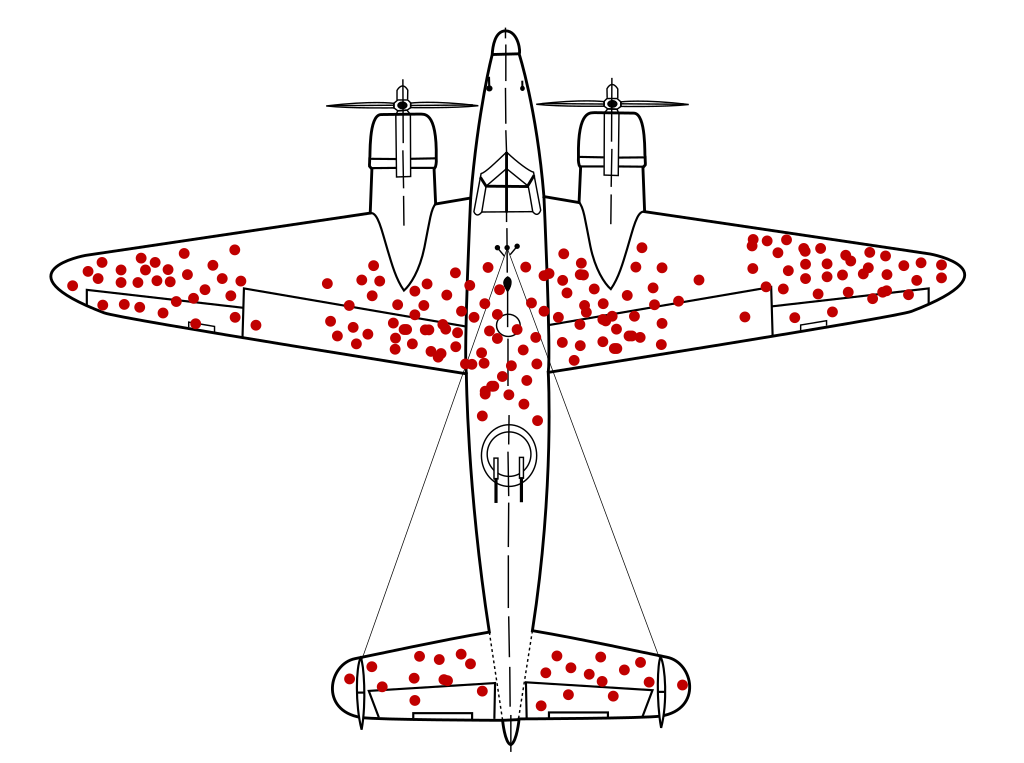
\includegraphics[width=0.37\textwidth]{../figures/survivorship}
  \end{figure}

  It is typically easier to determine where \textit{not} to make the edits. Certain regions, no matter their contents, will never yield a viable repair.
\end{frame}

\begin{frame}[fragile]{Edit location refinement: example}
  Let's prune states absorbing obviously impossible repair trajectories!\vspace{-0.5cm}
  \begin{figure}[H]
    \resizebox{\textwidth}{!}{
      \begin{tikzpicture}[
%->, % makes the edges directed
        >=stealth',
        node distance=2.5cm, % specifies the minimum distance between two nodes. Change if necessary.
%  every state/.style={thick, fill=gray!10}, % sets the properties for each ’state’ node
        initial text=$ $, % sets the text that appears on the start arrow
      ]
        \node[state, initial]                (00) {$q_{0,0}$};
        \node[state, right of=00]            (10) {$q_{1,0}$};
        \node[accepting, state, right of=10] (20) {$q_{2,0}$};
%        \node[accepting, state, right of=20] (30) {$q_{3,0}$};
%        \node[accepting, state, right of=30] (40) {$q_{4,0}$};
%        \node[accepting, state, right of=40] (50) {$q_{5,0}$};

        \node[state, above of=00, shift={(-2cm,0cm)}] (01) {$q_{0,1}$};
        \node[state, right of=01]                          (11) {$q_{1,1}$};
        \node[state, right of=11]                          (21) {$q_{2,1}$};
        \node[accepting, state, right of=21]               (31) {$q_{3,1}$};
        \node[accepting, state, right of=31]               (41) {$q_{4,1}$};
        \node[accepting, state, right of=41]               (51) {$q_{5,1}$};

        \node[state, above of=01, shift={(-2cm,0cm)}] (0j) {$q_{0,2}$};
        \node[state, right of=0j]                          (1j) {$q_{1,2}$};
        \node[state, right of=1j]                          (2j) {$q_{2,2}$};
        \node[state, right of=2j]                          (3j) {$q_{3,2}$};
        \node[accepting, state, right of=3j]               (4j) {$q_{4,2}$};
        \node[accepting, state, right of=4j]               (5j) {$q_{5,2}$};

        \phantom{\node[state, above of=0j, shift={(-2cm,0cm)}] (0k) {$q_{0,3}$};}
        \phantom{\node[state, right of=0k]                         (1k) {$q_{1,3}$};}
        \phantom{\node[state, right of=1k]                         (2k) {$q_{2,3}$};}
        \node[state, right of=2k]                         (3k) {$q_{3,3}$};
        \node[state, right of=3k]                         (4k) {$q_{4,3}$};
        \node[accepting, state, right of=4k]              (5k) {$q_{5,3}$};

        \draw [->] (00) edge[below] node{$\sigma_1$} (10);
        \draw [->] (10) edge[below] node{$\sigma_2$} (20);
%        \draw [->] (20) edge[below] node{$\sigma_3$} (30);
%        \draw [->] (30) edge[below] node{$\sigma_4$} (40);
%        \draw [->] (40) edge[below] node{$\sigma_5$} (50);

        \draw [->] (01) edge[below] node{$\sigma_1$} (11);
        \draw [->] (11) edge[below] node[shift={(-0.2cm,0cm)}]{$\sigma_2$} (21);
        \draw [->] (21) edge[below] node[shift={(-0.2cm,0cm)}]{$\sigma_3$} (31);
        \draw [->] (31) edge[below] node[shift={(-0.2cm,0cm)}]{$\sigma_4$} (41);
        \draw [->] (41) edge[below] node{$\sigma_5$} (51);

        \draw [->] (0j) edge[below] node{$\sigma_1$} (1j);
        \draw [->] (1j) edge[below] node{$\sigma_2$} (2j);
        \draw [->] (2j) edge[below] node{$\sigma_3$} (3j);
        \draw [->] (3j) edge[below] node{$\sigma_4$} (4j);
        \draw [->] (4j) edge[below] node{$\sigma_5$} (5j);

%        \draw [->] (0k) edge[below] node{$\sigma_1$} (1k);
%        \draw [->] (1k) edge[below] node{$\sigma_2$} (2k);
%        \draw [->] (2k) edge[below] node{$\sigma_3$} (3k);
        \draw [->] (3k) edge[below] node{$\sigma_4$} (4k);
        \draw [->] (4k) edge[below] node{$\sigma_5$} (5k);

        \draw [->] (00) edge[left] node{$\phantom{\cdot}$} (11);
        \draw [->] (10) edge[left] node{$\phantom{\cdot}$} (21);
        \draw [->] (20) edge[left] node{$\phantom{\cdot}$} (31);
%        \draw [->] (30) edge[left] node{$\phantom{\cdot}$} (41);
%        \draw [->] (40) edge[left] node{$\phantom{\cdot}$} (51);

% Super-knight arcs
        \draw [->, red] (00) edge[bend right=8] node[east, shift={(-0.2cm,-0.7cm)}]{$\color{red}\sigma_3$}         (3j);
        \draw [->, red] (10) edge[bend right=8] node[east, shift={(-0.2cm,-0.7cm)}]{$\color{red}\sigma_4$}         (4j);
        \draw [->, red] (20) edge[bend right=8] node[east, shift={(-0.2cm,-0.7cm)}]{$\color{red}\sigma_5$}         (5j);

        \draw [->, red] (01) edge[bend left=8] node[east, shift={(-0.2cm,-0.7cm)}]{$\color{red}\sigma_3$}         (3k);
        \draw [->, red] (11) edge[bend left=8] node[east, shift={(-0.2cm,-0.7cm)}]{$\color{red}\sigma_4$}         (4k);
        \draw [->, red] (21) edge[bend left=8] node[east, shift={(-0.2cm,-0.7cm)}]{$\color{red}\sigma_5$}         (5k);

        \draw [->, violet] (00) edge node[east, shift={(-0.1cm,-0.8cm)}]{$\color{violet}\sigma_4$}  (4k);
        \draw [->, violet] (10) edge node[east, shift={(-0.1cm,-0.8cm)}]{$\color{violet}\sigma_5$}  (5k);

        \draw [->] (01) edge[left] node{$\phantom{\cdot}$} (1j);
        \draw [->] (11) edge[left] node{$\phantom{\cdot}$} (2j);
        \draw [->] (21) edge[left] node{$\phantom{\cdot}$} (3j);
        \draw [->] (31) edge[left] node{$\phantom{\cdot}$} (4j);
        \draw [->] (41) edge[left] node{$\phantom{\cdot}$} (5j);

%        \draw [->] (0j) edge[left] node{$\phantom{\cdot}$} (1k);
%        \draw [->] (1j) edge[left] node{$\phantom{\cdot}$} (2k);
        \draw [->] (2j) edge[left] node{$\phantom{\cdot}$} (3k);
        \draw [->] (3j) edge[left] node{$\phantom{\cdot}$} (4k);
        \draw [->] (4j) edge[left] node{$\phantom{\cdot}$} (5k);

        \draw [->] (00) edge[bend left=10, left] node{$\phantom{\cdot}$} (01);
        \draw [->] (10) edge[bend left=10, left] node{$\phantom{\cdot}$} (11);
        \draw [->] (20) edge[bend left=10, left] node{$\phantom{\cdot}$} (21);
%        \draw [->] (30) edge[bend left=10, left] node{$\phantom{\cdot}$} (31);
%        \draw [->] (40) edge[bend left=10, left] node{$\phantom{\cdot}$} (41);
%        \draw [->] (50) edge[bend left=10, left] node{$\phantom{\cdot}$} (51);

        \draw [->] (01) edge[bend left=10, left] node{$\phantom{\cdot}$} (0j);
        \draw [->] (11) edge[bend left=10, left] node{$\phantom{\cdot}$} (1j);
        \draw [->] (21) edge[bend left=10, left] node{$\phantom{\cdot}$} (2j);
        \draw [->] (31) edge[bend left=10, left] node{$\phantom{\cdot}$} (3j);
        \draw [->] (41) edge[bend left=10, left] node{$\phantom{\cdot}$} (4j);
        \draw [->] (51) edge[bend left=10, left] node{$\phantom{\cdot}$} (5j);

%        \draw [->] (0j) edge[bend left=10, left] node{$\phantom{\cdot}$} (0k);
%        \draw [->] (1j) edge[bend left=10, left] node{$\phantom{\cdot}$} (1k);
%        \draw [->] (2j) edge[bend left=10, left] node{$\phantom{\cdot}$} (2k);
        \draw [->] (3j) edge[bend left=10, left] node{$\phantom{\cdot}$} (3k);
        \draw [->] (4j) edge[bend left=10, left] node{$\phantom{\cdot}$} (4k);
        \draw [->] (5j) edge[bend left=10, left] node{$\phantom{\cdot}$} (5k);

        \draw [->, blue] (00) edge[bend right=11,below] node[shift={(0.5cm,0.3cm)}]{$\color{blue}\sigma_2$}    (21);
        \draw [->, blue] (10) edge[bend right=11,below] node[shift={(0.5cm,0.3cm)}]{$\color{blue}\sigma_3$}    (31);
        \draw [->, blue] (20) edge[bend right=11,below] node[shift={(0.5cm,0.3cm)}]{$\color{blue}\sigma_4$}    (41);
%        \draw [->, blue] (30) edge[bend right=11,below] node[shift={(0.5cm,0.3cm)}]{$\color{blue}\sigma_5$}    (51);

        \draw [->, blue] (01) edge[bend right=3,below] node[shift={(0.3cm,0.2cm)}]{$\color{blue}\sigma_2$}    (2j);
        \draw [->, blue] (11) edge[bend right=3,below] node[shift={(0.3cm,0.2cm)}]{$\color{blue}\sigma_3$}    (3j);
        \draw [->, blue] (21) edge[bend right=3,below] node[shift={(0.3cm,0.2cm)}]{$\color{blue}\sigma_4$}    (4j);
        \draw [->, blue] (31) edge[bend right=3,below] node[shift={(0.3cm,0.2cm)}]{$\color{blue}\sigma_4$}    (5j);

%        \draw [->, blue] (0j) edge[bend left=8,below] node[shift={(-0.45cm,-0.55cm)}]{$\color{blue}\sigma_2$}    (2k);
        \draw [->, blue] (1j) edge[bend left=8,below] node[shift={(-0.45cm,-0.55cm)}]{$\color{blue}\sigma_3$}    (3k);
        \draw [->, blue] (2j) edge[bend left=8,below] node[shift={(-0.45cm,-0.55cm)}]{$\color{blue}\sigma_4$}    (4k);
        \draw [->, blue] (3j) edge[bend left=8,below] node[shift={(-0.45cm,-0.55cm)}]{$\color{blue}\sigma_5$}    (5k);

%https://tex.stackexchange.com/a/20986/139648
%        \draw [decorate,decoration={brace,amplitude=10pt,raise=10pt,mirror}] (00.south west) -- (50.south east) node[midway,yshift=-3em]{\textbf{String length}};
%        \draw [decorate,decoration={brace,amplitude=10pt,raise=20pt}] (00.south west) -- (0k.north west) node[midway,xshift=-1cm,yshift=-1cm,rotate=-54]{\textbf{Edit distance}};
      \end{tikzpicture}
    }
  \end{figure}

  $G$: \texttt{S $\rightarrow$ ( S ) |}\hspace{1.4cm}$\sigma$: \texttt{[ ( + ) ]}\phantom{...}\emoji{cross-mark}\\
  \phantom{$G$: \texttt{S $\rightarrow$ }}\texttt{[ S ] |}\phantom{\texttt{S ) }... $\sigma$: }\texttt{\_ \_ + ) ]}\phantom{...}\emoji{cross-mark}\phantom{...} $\land$ \phantom{...}\texttt{\_ \_ \_ ) ]}\phantom{...}\emoji{check-mark-button}\\
  \phantom{$G$: \texttt{S $\rightarrow$ }}\texttt{S + S | 1}\phantom{\texttt{ |}... $\sigma$: }\texttt{[ ( + \_ \_}\phantom{...}\emoji{cross-mark}\phantom{...} $\land$ \phantom{...}\texttt{[ ( \_ \_ \_}\phantom{...}\emoji{check-mark-button}
\end{frame}

\begin{frame}[fragile]{Grammar refinement: Parikh interval maps}
  If we’re reusing the CFG, it makes sense to precompute some statistics. For example, the total tokens each nonterminal can parse.

%  e.g., if $R$ is a unit nonterminal that maps to one value, then $[R] = [1, 1]$. Can be parameterized by $\Sigma$., e.g.,: $[R] = \{a:[1,1], b:[0,0]\ldots\}$\\\vspace{0.5cm}

  \begin{definition}[Parikh map for nonterminals]
    The \textbf{Parikh image}, $p: \Sigma^* \rightarrow \mathbb{N}^{|\Sigma|}$, counts the number of times each terminal appears in a string. The \textbf{Parikh map}, $\pi: V \times \mathbb{N} \rightarrow \Pi$, is the smallest interval containing the Parikh image across all strings generated by a nonterminal $R$ of length $n$, i.e, $\forall \sigma \in \mathcal{L}(R) \cap \Sigma^n \vdash p(\sigma) \in \pi(R, n)$.
  \end{definition}

  Likewise, we can define a Parikh interval for subautomata.

  \begin{definition}[Parikh map for subautomata]
    The \textbf{Parikh map} for a subautomaton, $\pi: Q \times Q \rightarrow \Pi$, returns the smallest interval s.t. $\forall \sigma: \Sigma^*, q, q': Q, q \overset{\sigma}{\Longrightarrow} q' \vdash p(\sigma) \in \pi(q, q')$.
  \end{definition}

%  We call this the Parikh interval. We can compute it for each string length, e.g., $[R, a, 1] = \{a:[1,1], b:[0,0]\ldots\}, [R, a, 2] = \ldots$\\\vspace{0.5cm}

  Now when we have a new automaton, we can check whether $(q, v, q')$ is compatible by checking whether the Parikh range for q, q’ and v overlaps.\\\vspace{0.5cm}

%  This optimization is not specific to LBH intersections, and can be applied to any CFG/FSA intersection.
\end{frame}

\begin{frame}[fragile]{Grammar refinement: Parikh compatibility}
  Criteria to overapproximate compatible nonterminals and states:

  \begin{definition}[Parikh compatibility]
    We call a nonterminal $R$ and state pair $q, q'$ \textit{compatible} when:\\
    \begin{prooftree}
      \AxiomC{$\displaystyle\mathcal{L}(R) \cap \bigcup_{\mathclap{n \in \llbracket q, q' \rrbracket}}\Sigma^n \neq \varnothing $}
      \AxiomC{$\displaystyle\pi(q, q') \cap \bigcup_{\mathclap{n\in \llbracket q, q' \rrbracket}} \pi(R, n) \neq \varnothing$}
      \RightLabel{$\lhd$}
      \BinaryInfC{$R \lhd q, q'$}
    \end{prooftree}
    where $\llbracket q, q' \rrbracket = [\min |\sigma|, \max |\sigma|]$ s.t. $q \overset{\sigma}{\Longrightarrow} q'$.
  \end{definition}

  Now, we are ready to re[de]fine the original $\Join$ rule:

  \noindent\begin{prooftree}
             \AxiomC{$(w \rightarrow xz) \in P\vphantom{\overset{a}{\rightarrow}}$}
             \AxiomC{$p,q,r \in Q$}
             \RightLabel{$\Join$}
             \BinaryInfC{$\big(pwr\rightarrow (pxq)(qzr)\big) \in P_\cap$}
  \end{prooftree}
\end{frame}

\begin{frame}[fragile]{Grammar refinement: Parikh interval maps}
  Criteria to overapproximate compatible nonterminals and states:

  \begin{definition}[Parikh compatibility]
    We call a nonterminal $R$ and state pair $q, q'$ \textit{compatible} when:\\
    \begin{prooftree}
      \AxiomC{$\displaystyle\mathcal{L}(R) \cap \bigcup_{\mathclap{n \in \llbracket q, q' \rrbracket}}\Sigma^n \neq \varnothing $}
      \AxiomC{$\displaystyle\pi(q, q') \cap \bigcup_{\mathclap{n\in \llbracket q, q' \rrbracket}} \pi(R, n) \neq \varnothing$}
      \RightLabel{$\lhd$}
      \BinaryInfC{$R \lhd q, q'$}
    \end{prooftree}
    where $\llbracket q, q' \rrbracket = [\min |\sigma|, \max |\sigma|]$ s.t. $q \overset{\sigma}{\Longrightarrow} q'$.
  \end{definition}

  Now, we are ready to re[de]fine the original $\Join$ rule:

  \noindent\begin{prooftree}
   \def\defaultHypSeparation{\hskip 0.14cm}
   \AxiomC{$\vphantom{\overset{[\cdot]}{\rightarrow}}\color{orange} w \lhd pr \phantom{\land} x \lhd pq \phantom{\land} z \lhd qr$}
   \AxiomC{$(w \rightarrow xz) \in P\vphantom{\overset{a}{\rightarrow}}$}
   \AxiomC{$p,q,r \in Q$}
   \RightLabel{$\hat\Join$}
   \TrinaryInfC{$\big(pwr\rightarrow (pxq)(qzr)\big) \in P_\cap$}
  \end{prooftree}
\end{frame}

\begin{frame}[fragile]{Potential ambiguity of Levenshtein-Bar-Hillel grammars}
The previous technique enumerates parse trees in a given $\mathbb{T}_2$, but does not guarantee string uniqueness since the CFG may be ambiguous.

\begin{lemma}[Possible ambiguity of LBH grammar]\label{lemma:ambiguity}
If the FSA, $\alpha$, is ambiguous, the intersection CFG, $G_\cap$, can be ambiguous.
\end{lemma}

\begin{proof}
Let $\ell$ be the language defined by $G=\{S\rightarrow LR, L \rightarrow\texttt{(}, R \rightarrow\texttt{)}\}$, where $\alpha=L(\err\sigma, 2)$, the broken string $\err\sigma$ is $\texttt{)(}$, and $\mathcal{L}(G_\cap) = \ell \cap \mathcal{L}(\alpha)$. Then, $\mathcal{L}(G_\cap)$ contains the following two identical repairs: \texttt{\hlred{)}(\hlgreen{)}} with the parse $S \rightarrow q_{00}Lq_{21}\phantom{.}q_{21}Rq_{22}$, and \texttt{\hlorange{(}\hlorange{)}} with the parse $S \rightarrow q_{00}Lq_{11}\phantom{.}q_{11}Rq_{22}$.
\end{proof}

We can eliminate ambiguity and thereby improve the rate of convergence for natural syntax repair by first translating $\mathbb{T}_2$ into an FSA.
\end{frame}

\begin{frame}[fragile]{Existence of an FSA that generates $\mathcal{L}(G_\cap)$}
There is an FSA generating $\mathcal{L}(G_\cap)$. We first show this non-constructively:

\begin{lemma}[Acyclicity of LBH grammar]\label{lemma:upper-bound}
The intersection grammar, $G_\cap$, is acyclic.
\end{lemma}

\begin{proof}
Assume $G_\cap$ is cyclic. Then $\mathcal{L}(G_\cap)$ must be infinite. But since $G_\cap$ generates $\ell \cap \mathcal{L}(\alpha)$ by construction and $\alpha$ is acyclic, $\mathcal{L}(G_\cap)$ is necessarily finite. Therefore, $G_\cap$ must not be cyclic.
\end{proof}

Since $G_\cap$ is acyclic and thus finite, it must be representable as an FSA. Using an FSA for decoding has many advantages, notably, it can be efficiently minimized and decoded in order of n-gram likelihood using a Markov chain or standard pretrained autoregressive language model.
\end{frame}

\begin{frame}[fragile]{Translating from $T_2$ to a DFA}
Let $+, *: \mathcal{A}\times \mathcal{A} \rightarrow \mathcal{A}$ be automata operators satisfying the property $\mathcal{L}(A_1 + A_2) = \mathcal{L}(A_1)\cup\mathcal{L}(A_2)$, and $\mathcal{L}(A_1 * A_2) = \mathcal{L}(A_1)\times\mathcal{L}(A_2)$. We can translate $\mathbb{T}_2$ to $\mathcal{A}$, as follows, recalling FSAs are closed over $+, *$:

\begin{equation*}
\mathcal{Y}(T:\mathbb{T}_2) \mapsto \begin{cases}
\alpha \mid \mathcal{L}(\alpha) = \{T\} & T: \Sigma, \\
\sum_{\langle T_1, T_2\rangle \in \texttt{children}(T)} \mathcal{Y}(T_1)*\mathcal{Y}(T_2) & T: VL\big(V^2P(a)^2\big)
\end{cases}
\end{equation*}
%
In the case of LBH intersections, $\mathcal{Y}(G_\cap')$ yields $\alpha: \mathcal{A} \mid \mathcal{L}(\alpha) = \ell\cap L(\err\sigma, d)$, which can be minimized via Brzozowski's algorithm then decoded:

\begin{figure}[H]
\centering
\includegraphics[width=0.9\textwidth]{../popl2025/exampleDFA}
\caption{$L(\scriptsize{\texttt{NAME = NAME . NAME ( NUM : , NUM : )}}, 2) \cap \ell_\textsc{Python}$}
\end{figure}
\end{frame}

\section{Decoding}\label{sec:error-correction}

\begin{frame}[fragile]{Decoding the DFA in order of normalized log likelihood}
\vspace{-0.3cm}
\begin{algorithm}[H]
\caption{Steerable DFA walk}
\label{alg:adaptive}
\begin{algorithmic}[1]
\Require $\mathcal{A} = \langle Q, \Sigma, \delta, I, F\rangle$ DFA, $P_\theta: \Sigma^d \rightarrow \mathbb{R}$ Markov chain

\State $\mathcal{T} \gets \varnothing \text{ total trajectories}, \mathcal{P} \gets \big[\langle \varepsilon, i, 0\rangle \mid i \in I\big] \text{ partial trajectories}$
%\State $[\mathcal{T, P}]\texttt{.comparator} = \lambda\langle\sigma, q, \gamma\rangle.(\frac{\gamma}{|\sigma|})$
\Repeat
\State \textbf{let }$\langle \sigma, q, \gamma \rangle = \texttt{head}(\mathcal{P})$ \textbf{in}
%\State $\mathcal{P} \gets \texttt{tail}(\mathcal{P})$
% For loop:
\State \phantom{\textbf{let }}$\mathbf{T} = \big\{\langle s\sigma, q', \gamma - \log P_\theta(s \mid \sigma_{1..d-1}) \rangle\mid (q\overset{s}{\rightarrow}q') \in \delta\big\}$
\For{$\langle \sigma, q, \gamma \rangle = T \in \mathbf{T}$}
\If {$\exists s: \Sigma, q': Q \mid (q\overset{s}{\rightarrow} q')\in\delta$}
\State $\mathcal{P} \gets \texttt{tail}(\mathcal{P}) \oplus T$ \Comment{Add partial trajectory to PQ.}
\EndIf
\If {$q \in F$}
\State $\mathcal{T} \gets \mathcal{T} \oplus T$ \Comment{Accepting state reached, add to queue.}
\EndIf
\EndFor
\Until{interrupted or $\mathcal{P}=\varnothing$.}
\State \Return $\big[\sigma_{|\sigma|..1} \mid \langle \sigma, q, \gamma \rangle = T \in \mathcal{T}\big]$ \Comment{Return in sorted order}
\end{algorithmic}
\end{algorithm}
\end{frame}

\begin{frame}[fragile]{Characteristics of the repair dataset}
\begin{figure}[h!]
\begin{tikzpicture}[scale=0.52]
\begin{axis}[
ybar,
bar width=5pt,
xlabel={Length $(|\err\sigma|)$},
ylabel={Frequency},
title={Cumulative length distribution},
axis x line*=bottom,
axis y line*=left,
ymin=0,
ymax=65,
xtick=data,
xticklabels={,,<30,,,<60,,,<90,},
ymajorgrids=true,
grid style=dashed,
width=0.45\textwidth,
height=0.3\textwidth
]

\addplot[fill=black!30] table {
X Y
1 7.60
2 14.52
3 22.01
4 30.54
5 37.82
6 44.30
7 49.68
8 55.21
9 59.75
10 63.59
};
\draw[red, dashed] (axis cs:8.5,0) -- (axis cs:8.5,65);
\end{axis}
\end{tikzpicture}
\begin{tikzpicture}[scale=0.52]
\begin{axis}[
ybar,
bar width=5pt,
title={Human repair distance},
xlabel={Edits, $\Delta(\err\sigma, \sigma')$},
ylabel={Frequency},
axis x line*=bottom,
axis y line*=left,
xtick=data,
ymajorgrids=true,
grid style=dashed,
xticklabels={,\leq 2,,\leq 4,,\leq 6,,\leq 8,,\leq 10},
ytick={0, 20, 40, 60, 80, 100},
ymin=0,
width=0.45\textwidth,
height=0.3\textwidth
]
\addplot[fill=black!30] table {
X Y
1  31.48
2  47.52
3  54.89
4  60.44
5  63.88
6  66.38
7  68.02
8  70.04
9  71.49
10 72.22
};
\draw[red, dashed] (axis cs:4.5,0) -- (axis cs:4.5,80);
\end{axis}
\end{tikzpicture}
\begin{tikzpicture}[scale=0.52]
\begin{axis}[
ybar,
bar width=5pt,
xlabel={Beginning $\longleftrightarrow$ End},
ylabel={Frequency},
title={Normalized edit locations},
axis x line*=bottom,
axis y line*=left,
ymin=0,
ymax=35,
xtick=data,
xticklabels={0\%,,,,,,,,,100\%},
ymajorgrids=true,
grid style=dashed,
width=0.45\textwidth,
height=0.3\textwidth
]

\addplot[fill=black!30] table {
X Y
10 11.6539
20 5.7252
30 6.2087
40 5.9542
50 5.5980
60 7.9389
70 7.0738
80 6.9466
90 12.4173
100 30.4835
};
\end{axis}
\end{tikzpicture}
%    \begin{tikzpicture}
%      \begin{axis}[
%        ybar,
%        bar width=5pt,
%        title={Intra-patch edit distance},
%        xlabel={Caret distance},
%        ylabel={Frequency},
%        axis x line*=bottom,
%        axis y line*=left,
%        xtick=data,
%        ymajorgrids=true,
%        grid style=dashed,
%        xticklabels={1,2,3,4,5,6,7,8,9,10+},
%        width=0.45\textwidth,
%        height=0.3\textwidth
%      ]
%
%        \addplot table {
%          X Y
%          1 40.66
%          2 15.00
%          3 5.80
%          4 4.86
%          5 4.26
%          6 2.98
%          7 2.05
%          8 2.73
%          9 1.62
%          10 13.64
%        };
%      \end{axis}
%    \end{tikzpicture}
\begin{tikzpicture}[scale=0.52]
\begin{axis}[
legend cell align={left},
legend style={fill opacity=1, draw opacity=1, text opacity=1, draw=lightgray204, legend columns=-1, legend pos=north east, legend style={at={(0.5,1.8)},anchor=north}},
xlabel={$|\err\sigma|$},
ylabel={Stable region},
title={Stability profile},
ybar,
axis lines*=left,
xtick={0, 10, 20, 30, 40, 50, 60, 70},
ytick={0, 0.2, 0.4, 0.6, 0.8, 1.0},
xticklabels={, {[}10{,}20{)}, , {[}30{,}40{)}, , {[}50{,}60{)}, , {[}70{,}80{)}},
yticklabels={0, 0.2, 0.4, 0.6, 0.8, 1.0},
x tick label style={font=\scriptsize},
ymax=1.0,
ymin=0.0,
bar width=3pt,
grid style=dashed,
ymajorgrids=true,
width=0.45\textwidth,
height=0.3\textwidth
]
\addlegendimage{empty legend}
\addlegendentry{$\Delta(\err\sigma, \sigma')=$}
\addlegendimage{ybar,ybar legend,draw=none,green,fill=green!50}
\addlegendentry{1,}
\addlegendimage{ybar,ybar legend,draw=none,blue,fill=blue!50}
\addlegendentry{2,}
\addlegendimage{ybar,ybar legend,draw=none,orange,fill=orange!50}
\addlegendentry{3}
\addplot[green, fill=green!50] coordinates {(0, 0.80) (10, 0.91) (20, 0.96) (30, 0.97) (40, 0.99) (50, 0.99) (60, 0.99) (70, 0.99)};
\addplot[blue, fill=blue!50] coordinates {(0, 0.35) (10, 0.59) (20, 0.69) (30, 0.73) (40, 0.79) (50, 0.82) (60, 0.84) (70, 0.86)};
\addplot[orange, fill=orange!50] coordinates {(0, 0.23) (10, 0.45) (20, 0.58) (30, 0.66) (40, 0.70) (50, 0.77) (60, 0.78) (70, 0.86)};
\end{axis}
\end{tikzpicture}
\caption{Repair statistics across the StackOverflow dataset, of which Tidyparse can handle about half in under $\sim$30s and $\sim$150 GB. Larger repairs and edit distances are possible, albeit requiring additional time and memory. The stability profile measures the average fraction of all edit locations that were never altered by any repair in the $L\big(\err\sigma, \Delta(\err\sigma, \sigma')\big)$-ball across repairs of varying length and distance.}\label{fig:patch_stats}
\end{figure}
\end{frame}

\begin{frame}[fragile]{Ranked repair}
We train on lexical n-grams using the standard MLE for Markov chains. To score the repairs, we use the conventional length-normalized NLL:

\begin{equation}
\text{NLL}(\sigma) = -\frac{1}{|\sigma|}\sum_{i=1}^{|\sigma|}\log P_\theta(\sigma_i \mid \sigma_{i-1}\ldots\sigma_{i-n})
\end{equation}

For each retrieved set $\hat{A} \subseteq A$ drawn before a predetermined timeout and each $\sigma \in \hat{A}$, we score the repair and return $\hat{A}$ in ascending order.

To evaluate the quality of our ranking, we use the Precision@k statistic. Specifically, given a repair model, $R: \Sigma^* \rightarrow 2^{\Sigma^*}$ and a parallel corpus, $\mathcal{D}_{\text{test}}$, of errors ($\sigma^\dagger$) and repairs ($\sigma'$), we define Precision@k as:

\begin{equation}
\text{Precision@k}(R) = \frac{1}{|\mathcal{D}_{\text{test}}|}\sum_{\langle\sigma^\dagger, \sigma'\rangle \in \mathcal{D}_{\text{test}}} \mathds{1}\big[\sigma' \in \argmax_{\bm{\sigma} \subset R(\sigma^\dagger), |\bm{\sigma}| \leq k}\sum_{\sigma \in \bm{\sigma}}\text{NLL}(\sigma)\big]
\end{equation}
\end{frame}

\begin{frame}[fragile]{Precision and latency comparison}
\begin{figure}[h!]
\resizebox{.24\textwidth}{!}{\input{../popl2025/len_dist_tidy}}
\resizebox{.24\textwidth}{!}{\begin{tikzpicture}
  \begin{axis}[
  xlabel={Snippet length, $|\sigma|$},
  ylabel={Precision@20k},
  title={\textbf{BIFI Repair Precision@20k}},
  legend cell align={left},
  legend style={fill opacity=0.8, draw opacity=1, text opacity=1, draw=lightgray204, legend columns=-1, legend pos=north east},
  ybar,
  axis lines*=left,
  xtick={0, 10, 20, 30, 40, 50, 60, 70},
  ytick={0, 0.1, 0.2, 0.3, 0.4, 0.5, 0.6, 0.7, 0.8, 0.9, 1.0},
  xticklabels={{(}0{,}10{)}, {[}10{,}20{)}, {[}20{,}30{)}, {[}30{,}40{)}, {[}40{,}50{)}, {[}50{,}60{)}, {[}60{,}70{)}, {[}70{,}80{)}},
  x tick label style={font=\scriptsize},
  ymax=1.0,
  ymin=0.0,
  bar width=4pt,
  ]

  \addlegendimage{empty legend}
  \addlegendentry{$\Delta(\err\sigma, \sigma')=$}
  \addlegendimage{ybar,ybar legend,draw=none,green,fill=green!50}
  \addlegendentry{1,}
  \addlegendimage{ybar,ybar legend,draw=none,blue,fill=blue!50}
  \addlegendentry{2,}
  \addlegendimage{ybar,ybar legend,draw=none,orange,fill=orange!50}
  \addlegendentry{3}

  \addplot[green, fill=green!50] coordinates   {(0, 0.65) (10, 0.67) (20, 0.71) (30, 0.63) (40, 0.60) (50, 0.62) (60, 0.59) (70, 0.64)};
  \addplot[blue, fill=blue!50] coordinates     {(0, 0.52) (10, 0.41) (20, 0.35) (30, 0.31) (40, 0.27) (50, 0.27) (60, 0.21) (70, 0.22)};
  \addplot[orange, fill=orange!50] coordinates {(0, 0.25) (10, 0.08) (20, 0.08) (30, 0.17) (40, 0.11) (50, 0.17) (60, 0.08) (70, 0.08)};

  \end{axis}
\end{tikzpicture}
}
\resizebox{.24\textwidth}{!}{\input{../popl2025/len_dist_s2p}}
\resizebox{.24\textwidth}{!}{\input{../popl2025/len_dist_bifi}}
\caption{Tidyparse, Seq2Parse and BIFI repair precision across length and edits.}
\end{figure}
\begin{figure}[h!]
%    \resizebox{.19\textwidth}{!}{\input{bar_hillel_repair.tex}}
\resizebox{.24\textwidth}{!}{% This file was created with tikzplotlib v0.10.1.
\begin{tikzpicture}
\begin{axis}[
legend cell align={left},
legend style={fill opacity=0.8, draw opacity=1, text opacity=1, draw=lightgray204, legend columns=-1, legend pos=north west},
tick align=outside,
tick pos=left,
axis lines*=left,
title={\(\displaystyle \Delta=1\) Repair Precision},
x grid style={darkgray176},
xlabel={Seconds},
xmin=-0.5925, xmax=8.5925,
xtick style={color=black},
xtick={0,1,2,3,4,5,6,7,8},
xticklabels={1,2,3,4,5,6,7,8,9},
y grid style={darkgray176},
ylabel={Precision@k},
ymin=0, ymax=1.03845,
ytick style={color=black}
]
\draw[draw=none,fill=darkviolet1270255] (axis cs:-0.175,0) rectangle (axis cs:0.175,0.619);
\addlegendimage{empty legend}
\addlegendentry{P@}
\addlegendimage{ybar,ybar legend,draw=none,fill=darkviolet1270255}
\addlegendentry{All}

\draw[draw=none,fill=darkviolet1270255] (axis cs:0.825,0) rectangle (axis cs:1.175,0.781);
\draw[draw=none,fill=darkviolet1270255] (axis cs:1.825,0) rectangle (axis cs:2.175,0.891);
\draw[draw=none,fill=darkviolet1270255] (axis cs:2.825,0) rectangle (axis cs:3.175,0.956);
\draw[draw=none,fill=darkviolet1270255] (axis cs:3.825,0) rectangle (axis cs:4.175,0.976);
\draw[draw=none,fill=darkviolet1270255] (axis cs:4.825,0) rectangle (axis cs:5.175,0.982);
\draw[draw=none,fill=darkviolet1270255] (axis cs:5.825,0) rectangle (axis cs:6.175,0.985);
\draw[draw=none,fill=darkviolet1270255] (axis cs:6.825,0) rectangle (axis cs:7.175,0.988);
\draw[draw=none,fill=darkviolet1270255] (axis cs:7.825,0) rectangle (axis cs:8.175,0.989);
\draw[draw=none,fill=royalblue8762253] (axis cs:-0.175,0) rectangle (axis cs:0.175,0.434);
\addlegendimage{ybar,ybar legend,draw=none,fill=royalblue8762253}
\addlegendentry{10}

\draw[draw=none,fill=royalblue8762253] (axis cs:0.825,0) rectangle (axis cs:1.175,0.556);
\draw[draw=none,fill=royalblue8762253] (axis cs:1.825,0) rectangle (axis cs:2.175,0.64);
\draw[draw=none,fill=royalblue8762253] (axis cs:2.825,0) rectangle (axis cs:3.175,0.69);
\draw[draw=none,fill=royalblue8762253] (axis cs:3.825,0) rectangle (axis cs:4.175,0.707);
\draw[draw=none,fill=royalblue8762253] (axis cs:4.825,0) rectangle (axis cs:5.175,0.71);
\draw[draw=none,fill=royalblue8762253] (axis cs:5.825,0) rectangle (axis cs:6.175,0.712);
\draw[draw=none,fill=royalblue8762253] (axis cs:6.825,0) rectangle (axis cs:7.175,0.714);
\draw[draw=none,fill=royalblue8762253] (axis cs:7.825,0) rectangle (axis cs:8.175,0.715);
\draw[draw=none,fill=dodgerblue45123246] (axis cs:-0.175,0) rectangle (axis cs:0.175,0.406);
\addlegendimage{ybar,ybar legend,draw=none,fill=dodgerblue45123246}
\addlegendentry{5}

\draw[draw=none,fill=dodgerblue45123246] (axis cs:0.825,0) rectangle (axis cs:1.175,0.517);
\draw[draw=none,fill=dodgerblue45123246] (axis cs:1.825,0) rectangle (axis cs:2.175,0.6);
\draw[draw=none,fill=dodgerblue45123246] (axis cs:2.825,0) rectangle (axis cs:3.175,0.648);
\draw[draw=none,fill=dodgerblue45123246] (axis cs:3.825,0) rectangle (axis cs:4.175,0.663);
\draw[draw=none,fill=dodgerblue45123246] (axis cs:4.825,0) rectangle (axis cs:5.175,0.667);
\draw[draw=none,fill=dodgerblue45123246] (axis cs:5.825,0) rectangle (axis cs:6.175,0.668);
\draw[draw=none,fill=dodgerblue45123246] (axis cs:6.825,0) rectangle (axis cs:7.175,0.67);
\draw[draw=none,fill=dodgerblue45123246] (axis cs:7.825,0) rectangle (axis cs:8.175,0.671);
\draw[draw=none,fill=deepskyblue3176236] (axis cs:-0.175,0) rectangle (axis cs:0.175,0.316);
\addlegendimage{ybar,ybar legend,draw=none,fill=deepskyblue3176236}
\addlegendentry{1}

\draw[draw=none,fill=deepskyblue3176236] (axis cs:0.825,0) rectangle (axis cs:1.175,0.4);
\draw[draw=none,fill=deepskyblue3176236] (axis cs:1.825,0) rectangle (axis cs:2.175,0.467);
\draw[draw=none,fill=deepskyblue3176236] (axis cs:2.825,0) rectangle (axis cs:3.175,0.504);
\draw[draw=none,fill=deepskyblue3176236] (axis cs:3.825,0) rectangle (axis cs:4.175,0.515);
\draw[draw=none,fill=deepskyblue3176236] (axis cs:4.825,0) rectangle (axis cs:5.175,0.518);
\draw[draw=none,fill=deepskyblue3176236] (axis cs:5.825,0) rectangle (axis cs:6.175,0.519);
\draw[draw=none,fill=deepskyblue3176236] (axis cs:6.825,0) rectangle (axis cs:7.175,0.52);
\draw[draw=none,fill=deepskyblue3176236] (axis cs:7.825,0) rectangle (axis cs:8.175,0.52);
\addplot [red, thick] coordinates {(-0.8925,0.39) (14.8925,0.39)};
\addplot [orange, thick] coordinates {(-0.8925,0.24) (14.8925,0.24)};
\end{axis}

\end{tikzpicture}
}
\resizebox{.24\textwidth}{!}{% This file was created with tikzplotlib v0.10.1.
\begin{tikzpicture}
\begin{axis}[
tick align=outside,
tick pos=left,
axis lines=left,
title={\(\displaystyle \Delta=2\) Repair Precision},
x grid style={darkgray176},
xlabel={Seconds},
xmin=-0.5925, xmax=8.5925,
xtick style={color=black},
xtick={0,1,2,3,4,5,6,7,8},
xticklabels={1,2,3,4,5,6,7,8,9},
y grid style={darkgray176},
ylabel={Precision@k},
ymin=0, ymax=0.9471,
ytick style={color=black}
]
\draw[draw=none,fill=darkviolet1270255] (axis cs:0.825,0) rectangle (axis cs:1.175,0.48);
\draw[draw=none,fill=darkviolet1270255] (axis cs:1.825,0) rectangle (axis cs:2.175,0.597);
\draw[draw=none,fill=darkviolet1270255] (axis cs:2.825,0) rectangle (axis cs:3.175,0.68);
\draw[draw=none,fill=darkviolet1270255] (axis cs:3.825,0) rectangle (axis cs:4.175,0.748);
\draw[draw=none,fill=darkviolet1270255] (axis cs:4.825,0) rectangle (axis cs:5.175,0.802);
\draw[draw=none,fill=darkviolet1270255] (axis cs:5.825,0) rectangle (axis cs:6.175,0.842);
\draw[draw=none,fill=darkviolet1270255] (axis cs:6.825,0) rectangle (axis cs:7.175,0.874);
\draw[draw=none,fill=darkviolet1270255] (axis cs:7.825,0) rectangle (axis cs:8.175,0.902);
\draw[draw=none,fill=royalblue8762253] (axis cs:-0.175,0) rectangle (axis cs:0.175,0.147);

\draw[draw=none,fill=royalblue8762253] (axis cs:0.825,0) rectangle (axis cs:1.175,0.197);
\draw[draw=none,fill=royalblue8762253] (axis cs:1.825,0) rectangle (axis cs:2.175,0.221);
\draw[draw=none,fill=royalblue8762253] (axis cs:2.825,0) rectangle (axis cs:3.175,0.243);
\draw[draw=none,fill=royalblue8762253] (axis cs:3.825,0) rectangle (axis cs:4.175,0.261);
\draw[draw=none,fill=royalblue8762253] (axis cs:4.825,0) rectangle (axis cs:5.175,0.274);
\draw[draw=none,fill=royalblue8762253] (axis cs:5.825,0) rectangle (axis cs:6.175,0.281);
\draw[draw=none,fill=royalblue8762253] (axis cs:6.825,0) rectangle (axis cs:7.175,0.29);
\draw[draw=none,fill=royalblue8762253] (axis cs:7.825,0) rectangle (axis cs:8.175,0.295);
\draw[draw=none,fill=dodgerblue45123246] (axis cs:-0.175,0) rectangle (axis cs:0.175,0.142);

\draw[draw=none,fill=dodgerblue45123246] (axis cs:0.825,0) rectangle (axis cs:1.175,0.19);
\draw[draw=none,fill=dodgerblue45123246] (axis cs:1.825,0) rectangle (axis cs:2.175,0.214);
\draw[draw=none,fill=dodgerblue45123246] (axis cs:2.825,0) rectangle (axis cs:3.175,0.234);
\draw[draw=none,fill=dodgerblue45123246] (axis cs:3.825,0) rectangle (axis cs:4.175,0.251);
\draw[draw=none,fill=dodgerblue45123246] (axis cs:4.825,0) rectangle (axis cs:5.175,0.263);
\draw[draw=none,fill=dodgerblue45123246] (axis cs:5.825,0) rectangle (axis cs:6.175,0.27);
\draw[draw=none,fill=dodgerblue45123246] (axis cs:6.825,0) rectangle (axis cs:7.175,0.278);
\draw[draw=none,fill=dodgerblue45123246] (axis cs:7.825,0) rectangle (axis cs:8.175,0.283);
\draw[draw=none,fill=deepskyblue3176236] (axis cs:-0.175,0) rectangle (axis cs:0.175,0.123);

\draw[draw=none,fill=deepskyblue3176236] (axis cs:0.825,0) rectangle (axis cs:1.175,0.16);
\draw[draw=none,fill=deepskyblue3176236] (axis cs:1.825,0) rectangle (axis cs:2.175,0.18);
\draw[draw=none,fill=deepskyblue3176236] (axis cs:2.825,0) rectangle (axis cs:3.175,0.196);
\draw[draw=none,fill=deepskyblue3176236] (axis cs:3.825,0) rectangle (axis cs:4.175,0.209);
\draw[draw=none,fill=deepskyblue3176236] (axis cs:4.825,0) rectangle (axis cs:5.175,0.219);
\draw[draw=none,fill=deepskyblue3176236] (axis cs:5.825,0) rectangle (axis cs:6.175,0.222);
\draw[draw=none,fill=deepskyblue3176236] (axis cs:6.825,0) rectangle (axis cs:7.175,0.227);
\draw[draw=none,fill=deepskyblue3176236] (axis cs:7.825,0) rectangle (axis cs:8.175,0.232);
\addplot [red, thick] coordinates {(-0.8925,0.15) (14.8925,0.15)};
\addplot [orange, thick] coordinates {(-0.8925,0.10) (14.8925,0.10)};
\end{axis}

\end{tikzpicture}
}
\resizebox{.24\textwidth}{!}{% This file was created with tikzplotlib v0.10.1.
\begin{tikzpicture}
\begin{axis}[
tick align=outside,
tick pos=left,
axis lines=left,
title={\(\displaystyle \Delta=3\) Repair Precision},
legend style={fill opacity=0.8, draw opacity=1, text opacity=1, legend columns=1, legend pos=north west},
x grid style={darkgray176},
xlabel={Seconds},
xmin=-0.5925, xmax=8.5925,
xtick style={color=black},
xtick={0,1,2,3,4,5,6,7,8},
xticklabels={10,20,30,40,50,60,70,80,90},
y grid style={darkgray176},
ylabel={Precision@k},
ymin=0, ymax=0.74655,
ytick style={color=black}
legend style={draw=none}
]
\draw[draw=none,fill=darkviolet1270255] (axis cs:0.825,0) rectangle (axis cs:1.175,0.372);
\draw[draw=none,fill=darkviolet1270255] (axis cs:1.825,0) rectangle (axis cs:2.175,0.472);
\draw[draw=none,fill=darkviolet1270255] (axis cs:2.825,0) rectangle (axis cs:3.175,0.543);
\draw[draw=none,fill=darkviolet1270255] (axis cs:3.825,0) rectangle (axis cs:4.175,0.59);
\draw[draw=none,fill=darkviolet1270255] (axis cs:4.825,0) rectangle (axis cs:5.175,0.625);
\draw[draw=none,fill=darkviolet1270255] (axis cs:5.825,0) rectangle (axis cs:6.175,0.655);
\draw[draw=none,fill=darkviolet1270255] (axis cs:6.825,0) rectangle (axis cs:7.175,0.69);
\draw[draw=none,fill=darkviolet1270255] (axis cs:7.825,0) rectangle (axis cs:8.175,0.711);
\draw[draw=none,fill=royalblue8762253] (axis cs:-0.175,0) rectangle (axis cs:0.175,0.117);

\draw[draw=none,fill=royalblue8762253] (axis cs:0.825,0) rectangle (axis cs:1.175,0.158);
\draw[draw=none,fill=royalblue8762253] (axis cs:1.825,0) rectangle (axis cs:2.175,0.204);
\draw[draw=none,fill=royalblue8762253] (axis cs:2.825,0) rectangle (axis cs:3.175,0.234);
\draw[draw=none,fill=royalblue8762253] (axis cs:3.825,0) rectangle (axis cs:4.175,0.254);
\draw[draw=none,fill=royalblue8762253] (axis cs:4.825,0) rectangle (axis cs:5.175,0.266);
\draw[draw=none,fill=royalblue8762253] (axis cs:5.825,0) rectangle (axis cs:6.175,0.273);
\draw[draw=none,fill=royalblue8762253] (axis cs:6.825,0) rectangle (axis cs:7.175,0.286);
\draw[draw=none,fill=royalblue8762253] (axis cs:7.825,0) rectangle (axis cs:8.175,0.291);
\draw[draw=none,fill=dodgerblue45123246] (axis cs:-0.175,0) rectangle (axis cs:0.175,0.111);

\draw[draw=none,fill=dodgerblue45123246] (axis cs:0.825,0) rectangle (axis cs:1.175,0.141);
\draw[draw=none,fill=dodgerblue45123246] (axis cs:1.825,0) rectangle (axis cs:2.175,0.183);
\draw[draw=none,fill=dodgerblue45123246] (axis cs:2.825,0) rectangle (axis cs:3.175,0.205);
\draw[draw=none,fill=dodgerblue45123246] (axis cs:3.825,0) rectangle (axis cs:4.175,0.223);
\draw[draw=none,fill=dodgerblue45123246] (axis cs:4.825,0) rectangle (axis cs:5.175,0.233);
\draw[draw=none,fill=dodgerblue45123246] (axis cs:5.825,0) rectangle (axis cs:6.175,0.241);
\draw[draw=none,fill=dodgerblue45123246] (axis cs:6.825,0) rectangle (axis cs:7.175,0.251);
\draw[draw=none,fill=dodgerblue45123246] (axis cs:7.825,0) rectangle (axis cs:8.175,0.256);
\draw[draw=none,fill=deepskyblue3176236] (axis cs:-0.175,0) rectangle (axis cs:0.175,0.076);

\draw[draw=none,fill=deepskyblue3176236] (axis cs:0.825,0) rectangle (axis cs:1.175,0.094);
\draw[draw=none,fill=deepskyblue3176236] (axis cs:1.825,0) rectangle (axis cs:2.175,0.113);
\draw[draw=none,fill=deepskyblue3176236] (axis cs:2.825,0) rectangle (axis cs:3.175,0.119);
\draw[draw=none,fill=deepskyblue3176236] (axis cs:3.825,0) rectangle (axis cs:4.175,0.129);
\draw[draw=none,fill=deepskyblue3176236] (axis cs:4.825,0) rectangle (axis cs:5.175,0.134);
\draw[draw=none,fill=deepskyblue3176236] (axis cs:5.825,0) rectangle (axis cs:6.175,0.138);
\draw[draw=none,fill=deepskyblue3176236] (axis cs:6.825,0) rectangle (axis cs:7.175,0.143);
\draw[draw=none,fill=deepskyblue3176236] (axis cs:7.825,0) rectangle (axis cs:8.175,0.146);
\addplot [red, thick] coordinates {(-0.8925,0.07) (14.8925,0.07)};
\addplot [orange, thick] coordinates {(-0.8925,0.04) (14.8925,0.04)};
\end{axis}

\end{tikzpicture}
}
\resizebox{.24\textwidth}{!}{\input{../popl2025/bar_hillel_repair_4}}
%    \resizebox{.24\textwidth}{!}{\input{bar_hillel_repair_5}}
%\resizebox{.3\textwidth}{!}{% This file was created with tikzplotlib v0.10.1.
\begin{tikzpicture}

\definecolor{darkgray176}{RGB}{176,176,176}
\definecolor{darkviolet1270255}{RGB}{127,0,255}
\definecolor{deepskyblue3176236}{RGB}{3,176,236}
\definecolor{dodgerblue45123246}{RGB}{45,123,246}
\definecolor{lightgray204}{RGB}{204,204,204}
\definecolor{royalblue8762253}{RGB}{87,62,253}

\begin{axis}[
legend cell align={left},
legend style={fill opacity=0.8, draw opacity=1, text opacity=1, draw=lightgray204, legend columns=-1, legend pos=north west},
tick align=outside,
tick pos=left,
title={$\Delta=1$ Repair Precision},
x grid style={darkgray176},
xlabel={Seconds},
xmin=-0.4925, xmax=6.4925,
xtick style={color=black},
xtick={0,1,2,3,4,5,6},
xticklabels={20,60,100,140,180,220,260},
y grid style={darkgray176},
ylabel={\phantom{Precision@k}},
ymin=0, ymax=0.77595,
ytick style={color=black}
]
\addlegendimage{empty legend}
\addlegendentry{P@}
\draw[draw=none,fill=darkviolet1270255] (axis cs:-0.175,0) rectangle (axis cs:0.175,0.145);
\addlegendimage{ybar,ybar legend,draw=none,fill=darkviolet1270255}
\addlegendentry{All}

\draw[draw=none,fill=darkviolet1270255] (axis cs:0.825,0) rectangle (axis cs:1.175,0.304);
\draw[draw=none,fill=darkviolet1270255] (axis cs:1.825,0) rectangle (axis cs:2.175,0.42);
\draw[draw=none,fill=darkviolet1270255] (axis cs:2.825,0) rectangle (axis cs:3.175,0.507);
\draw[draw=none,fill=darkviolet1270255] (axis cs:3.825,0) rectangle (axis cs:4.175,0.594);
\draw[draw=none,fill=darkviolet1270255] (axis cs:4.825,0) rectangle (axis cs:5.175,0.71);
\draw[draw=none,fill=darkviolet1270255] (axis cs:5.825,0) rectangle (axis cs:6.175,0.739);
\draw[draw=none,fill=royalblue8762253] (axis cs:-0.175,0) rectangle (axis cs:0.175,0.145);
\addlegendimage{ybar,ybar legend,draw=none,fill=royalblue8762253}
\addlegendentry{10}

\draw[draw=none,fill=royalblue8762253] (axis cs:0.825,0) rectangle (axis cs:1.175,0.304);
\draw[draw=none,fill=royalblue8762253] (axis cs:1.825,0) rectangle (axis cs:2.175,0.42);
\draw[draw=none,fill=royalblue8762253] (axis cs:2.825,0) rectangle (axis cs:3.175,0.507);
\draw[draw=none,fill=royalblue8762253] (axis cs:3.825,0) rectangle (axis cs:4.175,0.594);
\draw[draw=none,fill=royalblue8762253] (axis cs:4.825,0) rectangle (axis cs:5.175,0.703);
\draw[draw=none,fill=royalblue8762253] (axis cs:5.825,0) rectangle (axis cs:6.175,0.732);
\draw[draw=none,fill=dodgerblue45123246] (axis cs:-0.175,0) rectangle (axis cs:0.175,0.145);
\addlegendimage{ybar,ybar legend,draw=none,fill=dodgerblue45123246}
\addlegendentry{5}

\draw[draw=none,fill=dodgerblue45123246] (axis cs:0.825,0) rectangle (axis cs:1.175,0.304);
\draw[draw=none,fill=dodgerblue45123246] (axis cs:1.825,0) rectangle (axis cs:2.175,0.42);
\draw[draw=none,fill=dodgerblue45123246] (axis cs:2.825,0) rectangle (axis cs:3.175,0.493);
\draw[draw=none,fill=dodgerblue45123246] (axis cs:3.825,0) rectangle (axis cs:4.175,0.565);
\draw[draw=none,fill=dodgerblue45123246] (axis cs:4.825,0) rectangle (axis cs:5.175,0.638);
\draw[draw=none,fill=dodgerblue45123246] (axis cs:5.825,0) rectangle (axis cs:6.175,0.667);
\draw[draw=none,fill=deepskyblue3176236] (axis cs:-0.175,0) rectangle (axis cs:0.175,0.116);
\addlegendimage{ybar,ybar legend,draw=none,fill=deepskyblue3176236}
\addlegendentry{1}

\draw[draw=none,fill=deepskyblue3176236] (axis cs:0.825,0) rectangle (axis cs:1.175,0.203);
\draw[draw=none,fill=deepskyblue3176236] (axis cs:1.825,0) rectangle (axis cs:2.175,0.268);
\draw[draw=none,fill=deepskyblue3176236] (axis cs:2.825,0) rectangle (axis cs:3.175,0.312);
\draw[draw=none,fill=deepskyblue3176236] (axis cs:3.825,0) rectangle (axis cs:4.175,0.355);
\draw[draw=none,fill=deepskyblue3176236] (axis cs:4.825,0) rectangle (axis cs:5.175,0.428);
\draw[draw=none,fill=deepskyblue3176236] (axis cs:5.825,0) rectangle (axis cs:6.175,0.442);
\end{axis}

\end{tikzpicture}
}
%\resizebox{.307\textwidth}{!}{% This file was created with tikzplotlib v0.10.1.
\begin{tikzpicture}

\definecolor{darkgray176}{RGB}{176,176,176}
\definecolor{darkviolet1270255}{RGB}{127,0,255}
\definecolor{deepskyblue3176236}{RGB}{3,176,236}
\definecolor{dodgerblue45123246}{RGB}{45,123,246}
\definecolor{lightgray204}{RGB}{204,204,204}
\definecolor{royalblue8762253}{RGB}{87,62,253}

\begin{axis}[
legend cell align={left},
legend style={fill opacity=0.8, draw opacity=1, text opacity=1, draw=lightgray204, legend columns=-1, legend pos=north west},
tick align=outside,
tick pos=left,
title={$\Delta=2$ Repair Precision},
x grid style={darkgray176},
xlabel={Seconds},
xmin=-0.4925, xmax=6.4925,
xtick style={color=black},
xtick={0,1,2,3,4,5,6},
xticklabels={20,60,100,140,180,220,260},
y grid style={darkgray176},
ylabel={\phantom{Precision@k}},
ymin=0, ymax=0.40635,
ytick style={color=black}
]
\addlegendimage{empty legend}
\addlegendentry{P@}
\draw[draw=none,fill=darkviolet1270255] (axis cs:-0.175,0) rectangle (axis cs:0.175,0.048);
\addlegendimage{ybar,ybar legend,draw=none,fill=darkviolet1270255}
\addlegendentry{All}

\draw[draw=none,fill=darkviolet1270255] (axis cs:0.825,0) rectangle (axis cs:1.175,0.081);
\draw[draw=none,fill=darkviolet1270255] (axis cs:1.825,0) rectangle (axis cs:2.175,0.177);
\draw[draw=none,fill=darkviolet1270255] (axis cs:2.825,0) rectangle (axis cs:3.175,0.274);
\draw[draw=none,fill=darkviolet1270255] (axis cs:3.825,0) rectangle (axis cs:4.175,0.306);
\draw[draw=none,fill=darkviolet1270255] (axis cs:4.825,0) rectangle (axis cs:5.175,0.355);
\draw[draw=none,fill=darkviolet1270255] (axis cs:5.825,0) rectangle (axis cs:6.175,0.387);
\draw[draw=none,fill=royalblue8762253] (axis cs:-0.175,0) rectangle (axis cs:0.175,0.048);
\addlegendimage{ybar,ybar legend,draw=none,fill=royalblue8762253}
\addlegendentry{10}

\draw[draw=none,fill=royalblue8762253] (axis cs:0.825,0) rectangle (axis cs:1.175,0.081);
\draw[draw=none,fill=royalblue8762253] (axis cs:1.825,0) rectangle (axis cs:2.175,0.113);
\draw[draw=none,fill=royalblue8762253] (axis cs:2.825,0) rectangle (axis cs:3.175,0.21);
\draw[draw=none,fill=royalblue8762253] (axis cs:3.825,0) rectangle (axis cs:4.175,0.226);
\draw[draw=none,fill=royalblue8762253] (axis cs:4.825,0) rectangle (axis cs:5.175,0.258);
\draw[draw=none,fill=royalblue8762253] (axis cs:5.825,0) rectangle (axis cs:6.175,0.242);
\draw[draw=none,fill=dodgerblue45123246] (axis cs:-0.175,0) rectangle (axis cs:0.175,0.048);
\addlegendimage{ybar,ybar legend,draw=none,fill=dodgerblue45123246}
\addlegendentry{5}

\draw[draw=none,fill=dodgerblue45123246] (axis cs:0.825,0) rectangle (axis cs:1.175,0.032);
\draw[draw=none,fill=dodgerblue45123246] (axis cs:1.825,0) rectangle (axis cs:2.175,0.065);
\draw[draw=none,fill=dodgerblue45123246] (axis cs:2.825,0) rectangle (axis cs:3.175,0.129);
\draw[draw=none,fill=dodgerblue45123246] (axis cs:3.825,0) rectangle (axis cs:4.175,0.113);
\draw[draw=none,fill=dodgerblue45123246] (axis cs:4.825,0) rectangle (axis cs:5.175,0.129);
\draw[draw=none,fill=dodgerblue45123246] (axis cs:5.825,0) rectangle (axis cs:6.175,0.113);
\draw[draw=none,fill=deepskyblue3176236] (axis cs:-0.175,0) rectangle (axis cs:0.175,0.016);
\addlegendimage{ybar,ybar legend,draw=none,fill=deepskyblue3176236}
\addlegendentry{1}

\draw[draw=none,fill=deepskyblue3176236] (axis cs:0.825,0) rectangle (axis cs:1.175,0);
\draw[draw=none,fill=deepskyblue3176236] (axis cs:1.825,0) rectangle (axis cs:2.175,0.016);
\draw[draw=none,fill=deepskyblue3176236] (axis cs:2.825,0) rectangle (axis cs:3.175,0.065);
\draw[draw=none,fill=deepskyblue3176236] (axis cs:3.825,0) rectangle (axis cs:4.175,0.048);
\draw[draw=none,fill=deepskyblue3176236] (axis cs:4.825,0) rectangle (axis cs:5.175,0.032);
\draw[draw=none,fill=deepskyblue3176236] (axis cs:5.825,0) rectangle (axis cs:6.175,0.032);
\end{axis}

\end{tikzpicture}
}
\caption{Latency benchmarks. Note the varying y-axis ranges. The red line marks Seq2Parse and the orange line marks BIFI's Precision@1 on the same repairs.}\label{fig:human}
\end{figure}
\end{frame}

\begin{frame}[fragile]{Results from sample efficiency experiments}
\begin{figure}[h!]
% This file was created with tikzplotlib v0.10.1.
\begin{tikzpicture}[scale=0.75]
\begin{axis}[
legend cell align={left},
legend style={fill opacity=0.8, draw opacity=1, text opacity=1, draw=lightgray204, legend columns=-1, legend pos=north west},
width=\textwidth,
height=.4\textwidth,
log basis x={10},
tick align=outside,
tick pos=left,
axis lines*=left,
title={\textbf{Uniform Sampling Efficiency}},
x grid style={darkgray176},
xlabel={Samples drawn (log scale)},
xmin=0.34892211545542, xmax=1001,
xmode=log,
%xtick style={color=black},
xtick={0.01,0.1,1,10,100,1000,10000},
xticklabels={
  \(\displaystyle 10^-2\),
  \(\displaystyle 10^-1\),
  \(\displaystyle 10^2\),
  \(\displaystyle 10^3\),
  \(\displaystyle 10^4\),
  \(\displaystyle 10^5\),
  \(\displaystyle 10^6\)
},
y grid style={darkgray176},
ylabel={Precision@All},
ymin=0, ymax=101,
%ytick style={color=black}
ytick={0,20,40,60,80,100}
]
\draw[draw=none,fill=green!80] (axis cs:-0.5,0) rectangle (axis cs:0.9,100);
\addlegendimage{empty legend}
\addlegendentry{$\Delta(\err\sigma, \sigma')=$}
\addlegendimage{ybar,ybar legend,draw=none,fill=green!80}
\addlegendentry{\footnotesize{$1,$}}
\addlegendimage{ybar,ybar legend,draw=none,fill=blue!80}
\addlegendentry{\footnotesize{$2,$}}
\addlegendimage{ybar,ybar legend,draw=none,fill=orange!80}
\addlegendentry{\footnotesize{$3$}}

\draw[draw=none,fill=green!80] (axis cs:0.1,0) rectangle (axis cs:1.9,100);
\draw[draw=none,fill=green!80] (axis cs:1.1,0) rectangle (axis cs:2.9,100);
\draw[draw=none,fill=green!80] (axis cs:2.1,0) rectangle (axis cs:3.9,100);
\draw[draw=none,fill=green!80] (axis cs:3.1,0) rectangle (axis cs:4.9,100);
\draw[draw=none,fill=green!80] (axis cs:4.1,0) rectangle (axis cs:5.9,100);
\draw[draw=none,fill=green!80] (axis cs:5.1,0) rectangle (axis cs:6.9,100);
\draw[draw=none,fill=green!80] (axis cs:6.1,0) rectangle (axis cs:7.9,100);
\draw[draw=none,fill=green!80] (axis cs:7.1,0) rectangle (axis cs:8.9,100);
\draw[draw=none,fill=green!80] (axis cs:8.1,0) rectangle (axis cs:9.9,100);
\draw[draw=none,fill=green!80] (axis cs:9.1,0) rectangle (axis cs:10.9,100);
\draw[draw=none,fill=green!80] (axis cs:10.1,0) rectangle (axis cs:11.9,100);
\draw[draw=none,fill=green!80] (axis cs:11.1,0) rectangle (axis cs:12.9,100);
\draw[draw=none,fill=green!80] (axis cs:12.1,0) rectangle (axis cs:13.9,100);
\draw[draw=none,fill=green!80] (axis cs:13.1,0) rectangle (axis cs:14.9,100);
\draw[draw=none,fill=green!80] (axis cs:14.1,0) rectangle (axis cs:15.9,100);
\draw[draw=none,fill=green!80] (axis cs:15.1,0) rectangle (axis cs:16.9,100);
\draw[draw=none,fill=green!80] (axis cs:16.1,0) rectangle (axis cs:17.9,100);
\draw[draw=none,fill=green!80] (axis cs:17.1,0) rectangle (axis cs:18.9,100);
\draw[draw=none,fill=green!80] (axis cs:18.1,0) rectangle (axis cs:19.9,100);
\draw[draw=none,fill=green!80] (axis cs:19.1,0) rectangle (axis cs:20.9,100);
\draw[draw=none,fill=green!80] (axis cs:20.1,0) rectangle (axis cs:21.9,100);
\draw[draw=none,fill=green!80] (axis cs:21.1,0) rectangle (axis cs:22.9,100);
\draw[draw=none,fill=green!80] (axis cs:22.1,0) rectangle (axis cs:23.9,100);
\draw[draw=none,fill=green!80] (axis cs:23.1,0) rectangle (axis cs:24.9,100);
\draw[draw=none,fill=green!80] (axis cs:24.1,0) rectangle (axis cs:25.9,100);
\draw[draw=none,fill=green!80] (axis cs:25.1,0) rectangle (axis cs:26.9,100);
\draw[draw=none,fill=green!80] (axis cs:26.1,0) rectangle (axis cs:27.9,100);
\draw[draw=none,fill=green!80] (axis cs:27.1,0) rectangle (axis cs:28.9,100);
\draw[draw=none,fill=green!80] (axis cs:28.1,0) rectangle (axis cs:29.9,100);
\draw[draw=none,fill=green!80] (axis cs:29.1,0) rectangle (axis cs:30.9,100);
\draw[draw=none,fill=green!80] (axis cs:30.1,0) rectangle (axis cs:31.9,100);
\draw[draw=none,fill=green!80] (axis cs:31.1,0) rectangle (axis cs:32.9,100);
\draw[draw=none,fill=green!80] (axis cs:32.1,0) rectangle (axis cs:33.9,100);
\draw[draw=none,fill=green!80] (axis cs:33.1,0) rectangle (axis cs:34.9,100);
\draw[draw=none,fill=green!80] (axis cs:34.1,0) rectangle (axis cs:35.9,100);
\draw[draw=none,fill=green!80] (axis cs:35.1,0) rectangle (axis cs:36.9,100);
\draw[draw=none,fill=green!80] (axis cs:36.1,0) rectangle (axis cs:37.9,100);
\draw[draw=none,fill=green!80] (axis cs:37.1,0) rectangle (axis cs:38.9,100);
\draw[draw=none,fill=green!80] (axis cs:38.1,0) rectangle (axis cs:39.9,100);
\draw[draw=none,fill=green!80] (axis cs:39.1,0) rectangle (axis cs:40.9,100);
\draw[draw=none,fill=green!80] (axis cs:40.1,0) rectangle (axis cs:41.9,100);
\draw[draw=none,fill=green!80] (axis cs:41.1,0) rectangle (axis cs:42.9,100);
\draw[draw=none,fill=green!80] (axis cs:42.1,0) rectangle (axis cs:43.9,100);
\draw[draw=none,fill=green!80] (axis cs:43.1,0) rectangle (axis cs:44.9,100);
\draw[draw=none,fill=green!80] (axis cs:44.1,0) rectangle (axis cs:45.9,100);
\draw[draw=none,fill=green!80] (axis cs:45.1,0) rectangle (axis cs:46.9,100);
\draw[draw=none,fill=green!80] (axis cs:46.1,0) rectangle (axis cs:47.9,100);
\draw[draw=none,fill=green!80] (axis cs:47.1,0) rectangle (axis cs:48.9,100);
\draw[draw=none,fill=green!80] (axis cs:48.1,0) rectangle (axis cs:49.9,100);
\draw[draw=none,fill=green!80] (axis cs:49.1,0) rectangle (axis cs:50.9,100);
\draw[draw=none,fill=green!80] (axis cs:50.1,0) rectangle (axis cs:51.9,100);
\draw[draw=none,fill=green!80] (axis cs:51.1,0) rectangle (axis cs:52.9,100);
\draw[draw=none,fill=green!80] (axis cs:52.1,0) rectangle (axis cs:53.9,100);
\draw[draw=none,fill=green!80] (axis cs:53.1,0) rectangle (axis cs:54.9,100);
\draw[draw=none,fill=green!80] (axis cs:54.1,0) rectangle (axis cs:55.9,100);
\draw[draw=none,fill=green!80] (axis cs:55.1,0) rectangle (axis cs:56.9,100);
\draw[draw=none,fill=green!80] (axis cs:56.1,0) rectangle (axis cs:57.9,100);
\draw[draw=none,fill=green!80] (axis cs:57.1,0) rectangle (axis cs:58.9,100);
\draw[draw=none,fill=green!80] (axis cs:58.1,0) rectangle (axis cs:59.9,100);
\draw[draw=none,fill=green!80] (axis cs:59.1,0) rectangle (axis cs:60.9,100);
\draw[draw=none,fill=green!80] (axis cs:60.1,0) rectangle (axis cs:61.9,100);
\draw[draw=none,fill=green!80] (axis cs:61.1,0) rectangle (axis cs:62.9,100);
\draw[draw=none,fill=green!80] (axis cs:62.1,0) rectangle (axis cs:63.9,100);
\draw[draw=none,fill=green!80] (axis cs:63.1,0) rectangle (axis cs:64.9,100);
\draw[draw=none,fill=green!80] (axis cs:64.1,0) rectangle (axis cs:65.9,100);
\draw[draw=none,fill=green!80] (axis cs:65.1,0) rectangle (axis cs:66.9,100);
\draw[draw=none,fill=green!80] (axis cs:66.1,0) rectangle (axis cs:67.9,100);
\draw[draw=none,fill=green!80] (axis cs:67.1,0) rectangle (axis cs:68.9,100);
\draw[draw=none,fill=green!80] (axis cs:68.1,0) rectangle (axis cs:69.9,100);
\draw[draw=none,fill=green!80] (axis cs:69.1,0) rectangle (axis cs:70.9,100);
\draw[draw=none,fill=green!80] (axis cs:70.1,0) rectangle (axis cs:71.9,100);
\draw[draw=none,fill=green!80] (axis cs:71.1,0) rectangle (axis cs:72.9,100);
\draw[draw=none,fill=green!80] (axis cs:72.1,0) rectangle (axis cs:73.9,100);
\draw[draw=none,fill=green!80] (axis cs:73.1,0) rectangle (axis cs:74.9,100);
\draw[draw=none,fill=green!80] (axis cs:74.1,0) rectangle (axis cs:75.9,100);
\draw[draw=none,fill=green!80] (axis cs:75.1,0) rectangle (axis cs:76.9,100);
\draw[draw=none,fill=green!80] (axis cs:76.1,0) rectangle (axis cs:77.9,100);
\draw[draw=none,fill=green!80] (axis cs:77.1,0) rectangle (axis cs:78.9,100);
\draw[draw=none,fill=green!80] (axis cs:78.1,0) rectangle (axis cs:79.9,100);
\draw[draw=none,fill=green!80] (axis cs:79.1,0) rectangle (axis cs:80.9,100);
\draw[draw=none,fill=green!80] (axis cs:80.1,0) rectangle (axis cs:81.9,100);
\draw[draw=none,fill=green!80] (axis cs:81.1,0) rectangle (axis cs:82.9,100);
\draw[draw=none,fill=green!80] (axis cs:82.1,0) rectangle (axis cs:83.9,100);

\draw[draw=none,fill=blue!80] (axis cs:0.1,0) rectangle (axis cs:1.9,19.7452229299363);
\draw[draw=none,fill=blue!80] (axis cs:1.1,0) rectangle (axis cs:2.9,26.7515923566879);
\draw[draw=none,fill=blue!80] (axis cs:2.1,0) rectangle (axis cs:3.9,31.5286624203822);
\draw[draw=none,fill=blue!80] (axis cs:3.1,0) rectangle (axis cs:4.9,35.3503184713376);
\draw[draw=none,fill=blue!80] (axis cs:4.1,0) rectangle (axis cs:5.9,38.2165605095541);
\draw[draw=none,fill=blue!80] (axis cs:5.1,0) rectangle (axis cs:6.9,40.4458598726115);
\draw[draw=none,fill=blue!80] (axis cs:6.1,0) rectangle (axis cs:7.9,44.9044585987261);
\draw[draw=none,fill=blue!80] (axis cs:7.1,0) rectangle (axis cs:8.9,48.0891719745223);
\draw[draw=none,fill=blue!80] (axis cs:8.1,0) rectangle (axis cs:9.9,51.5923566878981);
\draw[draw=none,fill=blue!80] (axis cs:9.1,0) rectangle (axis cs:10.9,54.7770700636943);
\draw[draw=none,fill=blue!80] (axis cs:10.1,0) rectangle (axis cs:11.9,57.6433121019108);
\draw[draw=none,fill=blue!80] (axis cs:11.1,0) rectangle (axis cs:12.9,58.5987261146497);
\draw[draw=none,fill=blue!80] (axis cs:12.1,2) rectangle (axis cs:13.9,61.1464968152866);
\draw[draw=none,fill=blue!80] (axis cs:13.1,2) rectangle (axis cs:14.9,63.3757961783439);
\draw[draw=none,fill=blue!80] (axis cs:14.1,4) rectangle (axis cs:15.9,66.8789808917197);
\draw[draw=none,fill=blue!80] (axis cs:15.1,4) rectangle (axis cs:16.9,69.7452229299363);
\draw[draw=none,fill=blue!80] (axis cs:16.1,6) rectangle (axis cs:17.9,70.3821656050955);
\draw[draw=none,fill=blue!80] (axis cs:17.1,6) rectangle (axis cs:18.9,72.9299363057325);
\draw[draw=none,fill=blue!80] (axis cs:18.1,6) rectangle (axis cs:19.9,75.1592356687898);
\draw[draw=none,fill=blue!80] (axis cs:19.1,6) rectangle (axis cs:20.9,76.1146496815287);
\draw[draw=none,fill=blue!80] (axis cs:20.1,8) rectangle (axis cs:21.9,78.343949044586);
\draw[draw=none,fill=blue!80] (axis cs:21.1,10) rectangle (axis cs:22.9,79.2993630573248);
\draw[draw=none,fill=blue!80] (axis cs:22.1,10) rectangle (axis cs:23.9,80.2547770700637);
\draw[draw=none,fill=blue!80] (axis cs:23.1,12) rectangle (axis cs:24.9,80.5732484076433);
\draw[draw=none,fill=blue!80] (axis cs:24.1,12) rectangle (axis cs:25.9,82.1656050955414);
\draw[draw=none,fill=blue!80] (axis cs:25.1,12) rectangle (axis cs:26.9,82.484076433121);
\draw[draw=none,fill=blue!80] (axis cs:26.1,12) rectangle (axis cs:27.9,82.8025477707006);
\draw[draw=none,fill=blue!80] (axis cs:27.1,14) rectangle (axis cs:28.9,84.0764331210191);
\draw[draw=none,fill=blue!80] (axis cs:28.1,14) rectangle (axis cs:29.9,85.6687898089172);
\draw[draw=none,fill=blue!80] (axis cs:29.1,14) rectangle (axis cs:30.9,86.3057324840764);
\draw[draw=none,fill=blue!80] (axis cs:30.1,16) rectangle (axis cs:31.9,86.3057324840764);
\draw[draw=none,fill=blue!80] (axis cs:31.1,16) rectangle (axis cs:32.9,87.5796178343949);
\draw[draw=none,fill=blue!80] (axis cs:32.1,16) rectangle (axis cs:33.9,89.171974522293);
\draw[draw=none,fill=blue!80] (axis cs:33.1,16) rectangle (axis cs:34.9,90.1273885350319);
\draw[draw=none,fill=blue!80] (axis cs:34.1,18) rectangle (axis cs:35.9,90.4458598726115);
\draw[draw=none,fill=blue!80] (axis cs:35.1,18) rectangle (axis cs:36.9,90.7643312101911);
\draw[draw=none,fill=blue!80] (axis cs:36.1,18) rectangle (axis cs:37.9,91.7197452229299);
\draw[draw=none,fill=blue!80] (axis cs:37.1,18) rectangle (axis cs:38.9,91.7197452229299);
\draw[draw=none,fill=blue!80] (axis cs:38.1,18) rectangle (axis cs:39.9,92.0382165605096);
\draw[draw=none,fill=blue!80] (axis cs:39.1,18) rectangle (axis cs:40.9,92.9936305732484);
\draw[draw=none,fill=blue!80] (axis cs:40.1,18) rectangle (axis cs:41.9,93.312101910828);
\draw[draw=none,fill=blue!80] (axis cs:41.1,18) rectangle (axis cs:42.9,93.312101910828);
\draw[draw=none,fill=blue!80] (axis cs:42.1,18) rectangle (axis cs:43.9,93.312101910828);
\draw[draw=none,fill=blue!80] (axis cs:43.1,20) rectangle (axis cs:44.9,93.6305732484076);
\draw[draw=none,fill=blue!80] (axis cs:44.1,20) rectangle (axis cs:45.9,95.2229299363057);
\draw[draw=none,fill=blue!80] (axis cs:45.1,20) rectangle (axis cs:46.9,95.2229299363057);
\draw[draw=none,fill=blue!80] (axis cs:46.1,22) rectangle (axis cs:47.9,95.2229299363057);
\draw[draw=none,fill=blue!80] (axis cs:47.1,22) rectangle (axis cs:48.9,95.2229299363057);
\draw[draw=none,fill=blue!80] (axis cs:48.1,22) rectangle (axis cs:49.9,95.2229299363057);
\draw[draw=none,fill=blue!80] (axis cs:49.1,22) rectangle (axis cs:50.9,95.5414012738854);
\draw[draw=none,fill=blue!80] (axis cs:50.1,22) rectangle (axis cs:51.9,95.5414012738854);
\draw[draw=none,fill=blue!80] (axis cs:51.1,24) rectangle (axis cs:52.9,96.1783439490446);
\draw[draw=none,fill=blue!80] (axis cs:52.1,26) rectangle (axis cs:53.9,96.1783439490446);
\draw[draw=none,fill=blue!80] (axis cs:53.1,26) rectangle (axis cs:54.9,96.1783439490446);
\draw[draw=none,fill=blue!80] (axis cs:54.1,26) rectangle (axis cs:55.9,96.1783439490446);
\draw[draw=none,fill=blue!80] (axis cs:55.1,26) rectangle (axis cs:56.9,96.1783439490446);
\draw[draw=none,fill=blue!80] (axis cs:56.1,26) rectangle (axis cs:57.9,96.8152866242038);
\draw[draw=none,fill=blue!80] (axis cs:57.1,26) rectangle (axis cs:58.9,97.1337579617834);
\draw[draw=none,fill=blue!80] (axis cs:58.1,26) rectangle (axis cs:59.9,97.1337579617834);
\draw[draw=none,fill=blue!80] (axis cs:59.1,26) rectangle (axis cs:60.9,97.1337579617834);
\draw[draw=none,fill=blue!80] (axis cs:60.1,26) rectangle (axis cs:61.9,97.1337579617834);
\draw[draw=none,fill=blue!80] (axis cs:61.1,26) rectangle (axis cs:62.9,97.4522292993631);
\draw[draw=none,fill=blue!80] (axis cs:62.1,26) rectangle (axis cs:63.9,98.0891719745223);
\draw[draw=none,fill=blue!80] (axis cs:63.1,26) rectangle (axis cs:64.9,98.0891719745223);
\draw[draw=none,fill=blue!80] (axis cs:64.1,26) rectangle (axis cs:65.9,98.4076433121019);
\draw[draw=none,fill=blue!80] (axis cs:65.1,26) rectangle (axis cs:66.9,98.7261146496815);
\draw[draw=none,fill=blue!80] (axis cs:66.1,26) rectangle (axis cs:67.9,98.7261146496815);
\draw[draw=none,fill=blue!80] (axis cs:67.1,26) rectangle (axis cs:68.9,98.7261146496815);
\draw[draw=none,fill=blue!80] (axis cs:68.1,26) rectangle (axis cs:69.9,99.0445859872611);
\draw[draw=none,fill=blue!80] (axis cs:69.1,26) rectangle (axis cs:70.9,99.0445859872611);
\draw[draw=none,fill=blue!80] (axis cs:70.1,26) rectangle (axis cs:71.9,99.0445859872611);
\draw[draw=none,fill=blue!80] (axis cs:71.1,26) rectangle (axis cs:72.9,99.0445859872611);
\draw[draw=none,fill=blue!80] (axis cs:72.1,26) rectangle (axis cs:73.9,99.3630573248408);
\draw[draw=none,fill=blue!80] (axis cs:73.1,26) rectangle (axis cs:74.9,99.3630573248408);
\draw[draw=none,fill=blue!80] (axis cs:74.1,26) rectangle (axis cs:75.9,99.3630573248408);
\draw[draw=none,fill=blue!80] (axis cs:75.1,28) rectangle (axis cs:76.9,99.3630573248408);
\draw[draw=none,fill=blue!80] (axis cs:76.1,28) rectangle (axis cs:77.9,99.3630573248408);
\draw[draw=none,fill=blue!80] (axis cs:77.1,28) rectangle (axis cs:78.9,99.6815286624204);
\draw[draw=none,fill=blue!80] (axis cs:78.1,30) rectangle (axis cs:786.9,100);

\draw[draw=none,fill=orange!80] (axis cs:12.0,0) rectangle (axis cs:14.99,2);
\draw[draw=none,fill=orange!80] (axis cs:14.0,0) rectangle (axis cs:15.99,4);
\draw[draw=none,fill=orange!80] (axis cs:15.0,0) rectangle (axis cs:16.99,4);
\draw[draw=none,fill=orange!80] (axis cs:16.0,0) rectangle (axis cs:17.99,6);
\draw[draw=none,fill=orange!80] (axis cs:17.0,0) rectangle (axis cs:18.99,6);
\draw[draw=none,fill=orange!80] (axis cs:18.0,0) rectangle (axis cs:19.99,6);
\draw[draw=none,fill=orange!80] (axis cs:19.0,0) rectangle (axis cs:20.99,6);
\draw[draw=none,fill=orange!80] (axis cs:20.0,0) rectangle (axis cs:21.99,8);
\draw[draw=none,fill=orange!80] (axis cs:21.0,0) rectangle (axis cs:22.99,10);
\draw[draw=none,fill=orange!80] (axis cs:22.0,0) rectangle (axis cs:23.99,10);
\draw[draw=none,fill=orange!80] (axis cs:23.0,0) rectangle (axis cs:24.99,12);
\draw[draw=none,fill=orange!80] (axis cs:24.0,0) rectangle (axis cs:25.99,12);
\draw[draw=none,fill=orange!80] (axis cs:25.0,0) rectangle (axis cs:26.99,12);
\draw[draw=none,fill=orange!80] (axis cs:26.0,0) rectangle (axis cs:27.99,12);
\draw[draw=none,fill=orange!80] (axis cs:27.0,0) rectangle (axis cs:28.99,14);
\draw[draw=none,fill=orange!80] (axis cs:28.0,0) rectangle (axis cs:29.99,14);
\draw[draw=none,fill=orange!80] (axis cs:29.0,0) rectangle (axis cs:30.99,14);
\draw[draw=none,fill=orange!80] (axis cs:30.0,0) rectangle (axis cs:31.99,16);
\draw[draw=none,fill=orange!80] (axis cs:31.0,0) rectangle (axis cs:32.99,16);
\draw[draw=none,fill=orange!80] (axis cs:32.0,0) rectangle (axis cs:33.99,16);
\draw[draw=none,fill=orange!80] (axis cs:33.0,0) rectangle (axis cs:34.99,16);
\draw[draw=none,fill=orange!80] (axis cs:34.0,0) rectangle (axis cs:43.99,18);
\draw[draw=none,fill=orange!80] (axis cs:43.0,0) rectangle (axis cs:44.99,20);
\draw[draw=none,fill=orange!80] (axis cs:44.0,0) rectangle (axis cs:45.99,20);
\draw[draw=none,fill=orange!80] (axis cs:45.0,0) rectangle (axis cs:46.99,20);
\draw[draw=none,fill=orange!80] (axis cs:46.0,0) rectangle (axis cs:47.99,22);
\draw[draw=none,fill=orange!80] (axis cs:47.0,0) rectangle (axis cs:48.99,22);
\draw[draw=none,fill=orange!80] (axis cs:48.0,0) rectangle (axis cs:49.99,22);
\draw[draw=none,fill=orange!80] (axis cs:49.0,0) rectangle (axis cs:50.99,22);
\draw[draw=none,fill=orange!80] (axis cs:50.0,0) rectangle (axis cs:51.99,22);
\draw[draw=none,fill=orange!80] (axis cs:51.0,0) rectangle (axis cs:52.99,24);
\draw[draw=none,fill=orange!80] (axis cs:52.0,0) rectangle (axis cs:75.99,26);
\draw[draw=none,fill=orange!80] (axis cs:75.0,0) rectangle (axis cs:76.99,28);
\draw[draw=none,fill=orange!80] (axis cs:76.0,0) rectangle (axis cs:77.99,28);
\draw[draw=none,fill=orange!80] (axis cs:77.0,0) rectangle (axis cs:78.99,28);
\draw[draw=none,fill=orange!80] (axis cs:78.0,0) rectangle (axis cs:79.99,30);
\draw[draw=none,fill=orange!80] (axis cs:79.0,0) rectangle (axis cs:80.99,30);
\draw[draw=none,fill=orange!80] (axis cs:80.0,0) rectangle (axis cs:81.99,30);
\draw[draw=none,fill=orange!80] (axis cs:81.0,0) rectangle (axis cs:82.99,30);
\draw[draw=none,fill=orange!80] (axis cs:82.0,0) rectangle (axis cs:83.99,30);
\draw[draw=none,fill=orange!80] (axis cs:83.0,0) rectangle (axis cs:84.99,30);
\draw[draw=none,fill=orange!80] (axis cs:84.0,0) rectangle (axis cs:85.99,30);
\draw[draw=none,fill=orange!80] (axis cs:85.0,0) rectangle (axis cs:86.99,32);
\draw[draw=none,fill=orange!80] (axis cs:86.0,0) rectangle (axis cs:87.99,32);
\draw[draw=none,fill=orange!80] (axis cs:87.0,0) rectangle (axis cs:88.99,32);
\draw[draw=none,fill=orange!80] (axis cs:88.0,0) rectangle (axis cs:89.99,32);
\draw[draw=none,fill=orange!80] (axis cs:89.0,0) rectangle (axis cs:90.99,32);
\draw[draw=none,fill=orange!80] (axis cs:90.0,0) rectangle (axis cs:91.99,32);
\draw[draw=none,fill=orange!80] (axis cs:91.0,0) rectangle (axis cs:116.99,36);
\draw[draw=none,fill=orange!80] (axis cs:116.0,0) rectangle (axis cs:130.99,38);
\draw[draw=none,fill=orange!80] (axis cs:130.0,0) rectangle (axis cs:138.99,40);
\draw[draw=none,fill=orange!80] (axis cs:138.0,0) rectangle (axis cs:139.99,42);
\draw[draw=none,fill=orange!80] (axis cs:139.0,0) rectangle (axis cs:140.99,42);
\draw[draw=none,fill=orange!80] (axis cs:140.0,0) rectangle (axis cs:141.99,42);
\draw[draw=none,fill=orange!80] (axis cs:141.0,0) rectangle (axis cs:142.99,42);
\draw[draw=none,fill=orange!80] (axis cs:142.0,0) rectangle (axis cs:143.99,42);
\draw[draw=none,fill=orange!80] (axis cs:143.0,0) rectangle (axis cs:144.99,42);
\draw[draw=none,fill=orange!80] (axis cs:144.0,0) rectangle (axis cs:145.99,42);
\draw[draw=none,fill=orange!80] (axis cs:145.0,0) rectangle (axis cs:170.99,44);
\draw[draw=none,fill=orange!80] (axis cs:170.0,0) rectangle (axis cs:191.99,46);
\draw[draw=none,fill=orange!80] (axis cs:191.0,0) rectangle (axis cs:192.99,48);
\draw[draw=none,fill=orange!80] (axis cs:192.0,0) rectangle (axis cs:193.99,48);
\draw[draw=none,fill=orange!80] (axis cs:193.0,0) rectangle (axis cs:194.99,48);
\draw[draw=none,fill=orange!80] (axis cs:194.0,0) rectangle (axis cs:195.99,48);
\draw[draw=none,fill=orange!80] (axis cs:195.0,0) rectangle (axis cs:196.99,48);
\draw[draw=none,fill=orange!80] (axis cs:196.0,0) rectangle (axis cs:197.99,48);
\draw[draw=none,fill=orange!80] (axis cs:197.0,0) rectangle (axis cs:211.99,50);
\draw[draw=none,fill=orange!80] (axis cs:211.0,0) rectangle (axis cs:212.99,52);
\draw[draw=none,fill=orange!80] (axis cs:212.0,0) rectangle (axis cs:213.99,52);
\draw[draw=none,fill=orange!80] (axis cs:213.0,0) rectangle (axis cs:214.99,52);
\draw[draw=none,fill=orange!80] (axis cs:214.0,0) rectangle (axis cs:215.99,56);
\draw[draw=none,fill=orange!80] (axis cs:215.0,0) rectangle (axis cs:216.99,56);
\draw[draw=none,fill=orange!80] (axis cs:216.0,0) rectangle (axis cs:217.99,56);
\draw[draw=none,fill=orange!80] (axis cs:217.0,0) rectangle (axis cs:218.99,56);
\draw[draw=none,fill=orange!80] (axis cs:218.0,0) rectangle (axis cs:219.99,56);
\draw[draw=none,fill=orange!80] (axis cs:219.0,0) rectangle (axis cs:220.99,56);
\draw[draw=none,fill=orange!80] (axis cs:220.0,0) rectangle (axis cs:221.99,56);
\draw[draw=none,fill=orange!80] (axis cs:221.0,0) rectangle (axis cs:222.99,56);
\draw[draw=none,fill=orange!80] (axis cs:222.0,0) rectangle (axis cs:223.99,56);
\draw[draw=none,fill=orange!80] (axis cs:223.0,0) rectangle (axis cs:224.99,56);
\draw[draw=none,fill=orange!80] (axis cs:224.0,0) rectangle (axis cs:236.99,58);
\draw[draw=none,fill=orange!80] (axis cs:236.0,0) rectangle (axis cs:247.99,60);
\draw[draw=none,fill=orange!80] (axis cs:247.0,0) rectangle (axis cs:288.99,64);
\draw[draw=none,fill=orange!80] (axis cs:288.0,0) rectangle (axis cs:289.99,68);
\draw[draw=none,fill=orange!80] (axis cs:289.0,0) rectangle (axis cs:290.99,68);
\draw[draw=none,fill=orange!80] (axis cs:290.0,0) rectangle (axis cs:304.99,70);
\draw[draw=none,fill=orange!80] (axis cs:304.0,0) rectangle (axis cs:305.99,72);
\draw[draw=none,fill=orange!80] (axis cs:305.0,0) rectangle (axis cs:306.99,72);
\draw[draw=none,fill=orange!80] (axis cs:306.0,0) rectangle (axis cs:307.99,72);
\draw[draw=none,fill=orange!80] (axis cs:307.0,0) rectangle (axis cs:308.99,72);
\draw[draw=none,fill=orange!80] (axis cs:308.0,0) rectangle (axis cs:309.99,74);
\draw[draw=none,fill=orange!80] (axis cs:309.0,0) rectangle (axis cs:310.99,74);
\draw[draw=none,fill=orange!80] (axis cs:310.0,0) rectangle (axis cs:311.99,74);
\draw[draw=none,fill=orange!80] (axis cs:311.0,0) rectangle (axis cs:366.99,76);
\draw[draw=none,fill=orange!80] (axis cs:366.0,0) rectangle (axis cs:394.99,78);
\draw[draw=none,fill=orange!80] (axis cs:394.0,0) rectangle (axis cs:415.99,80);
\draw[draw=none,fill=orange!80] (axis cs:415.0,0) rectangle (axis cs:416.99,82);
\draw[draw=none,fill=orange!80] (axis cs:416.0,0) rectangle (axis cs:440.99,84);
\draw[draw=none,fill=orange!80] (axis cs:440.0,0) rectangle (axis cs:490.99,86);
\draw[draw=none,fill=orange!80] (axis cs:490.0,0) rectangle (axis cs:513.99,88);
\draw[draw=none,fill=orange!80] (axis cs:513.0,0) rectangle (axis cs:522.99,90);
\draw[draw=none,fill=orange!80] (axis cs:522.0,0) rectangle (axis cs:554.99,92);
\draw[draw=none,fill=orange!80] (axis cs:554.0,0) rectangle (axis cs:583.99,94);
\draw[draw=none,fill=orange!80] (axis cs:583.0,0) rectangle (axis cs:597.99,96);
\draw[draw=none,fill=orange!80] (axis cs:597.0,0) rectangle (axis cs:786.99,98);
\end{axis}

\end{tikzpicture}\\
%    \caption{Sample efficiency of Tidyparse at varying Levenshtein radii. After drawing up to $\sim10^5$ samples without replacement we can usually retrieve the human repair for almost all repairs fewer than four edits.}\label{fig:sample_efficiency}
\resizebox{.35\textwidth}{!}{% This file was created with tikzplotlib v0.10.1.
\begin{tikzpicture}

  \definecolor{darkgray176}{RGB}{176,176,176}
  \definecolor{green}{RGB}{0,128,0}
  \definecolor{lightgray204}{RGB}{204,204,204}

  \begin{axis}[
  legend cell align={left},
  legend style={fill opacity=0.8, draw opacity=1, text opacity=1, draw=lightgray204},
  log basis y={10},
  tick align=outside,
  tick pos=left,
  title={Throughput across repair size},
  x grid style={darkgray176},
  xlabel={Lexical tokens},
  xmin=-0.95, xmax=19.95,
  xtick style={color=black},
  xtick={0,1,2,3,4,5,6,7,8,9,10,11,12,13,14,15,16,17,18},
  xticklabels={4, , 8, , 12, , 16, , 20, , 24, , 28, , 32, , 36, , 40},
  y grid style={darkgray176},
  ylabel={Total repairs discovered},
  ymin=26.9997073270017, ymax=114560.263215582,
  ymode=log,
  ytick style={color=black}
  ]
  \path [draw=blue, ]
  (axis cs:0,299.563426695481)
  --(axis cs:0,897.333125028657);

  \path [draw=blue, ]
  ;

  \path [draw=blue, ]
  (axis cs:2,954.594181243253)
  --(axis cs:2,2583.45459924455);

  \path [draw=blue, ]
  (axis cs:3,1128.52763702204)
  --(axis cs:3,2964.93182243742);

  \path [draw=blue, ]
  (axis cs:4,479.675101469012)
  --(axis cs:4,1034.6337220604);

  \path [draw=blue, ]
  (axis cs:5,459.881423316437)
  --(axis cs:5,1144.53687733716);

  \path [draw=blue, ]
  (axis cs:6,241.93755536542)
  --(axis cs:6,891.904868877004);

  \path [draw=blue, ]
  ;

  \path [draw=blue, ]
  (axis cs:8,239.447890447633)
  --(axis cs:8,535.162109552367);

  \path [draw=blue, ]
  (axis cs:9,273.691255767478)
  --(axis cs:9,532.450048580348);

  \path [draw=blue, ]
  (axis cs:10,199.424171801829)
  --(axis cs:10,388.874678772883);

  \path [draw=blue, ]
  (axis cs:11,185.933695381169)
  --(axis cs:11,449.376649446417);

  \path [draw=blue, ]
  ;

  \path [draw=blue, ]
  (axis cs:13,140.481202070267)
  --(axis cs:13,278.537202837709);

  \path [draw=blue, ]
  ;

  \path [draw=blue, ]
  (axis cs:15,130.976506510186)
  --(axis cs:15,300.526941765676);

  \path [draw=blue, ]
  ;

  \path [draw=blue, ]
  (axis cs:17,74.3394169879732)
  --(axis cs:17,212.761358205825);

  \path [draw=blue, ]
  (axis cs:18,144.350245595727)
  --(axis cs:18,358.641880388525);

  \path [draw=blue, ]
  ;

  \path [draw=green, ]
  (axis cs:0,332.087026352122)
  --(axis cs:0,571.03492486739);

  \path [draw=green, ]
  (axis cs:1,343.025446175718)
  --(axis cs:1,797.524004373732);

  \path [draw=green, ]
  (axis cs:2,337.633059565208)
  --(axis cs:2,449.672203592687);

  \path [draw=green, ]
  (axis cs:3,373.306323995034)
  --(axis cs:3,534.178705945085);

  \path [draw=green, ]
  (axis cs:4,349.095275484927)
  --(axis cs:4,454.718678003445);

  \path [draw=green, ]
  (axis cs:5,276.834148199237)
  --(axis cs:5,355.992106627017);

  \path [draw=green, ]
  (axis cs:6,267.328886318599)
  --(axis cs:6,374.603949502297);

  \path [draw=green, ]
  (axis cs:7,165.027785502998)
  --(axis cs:7,238.271825391944);

  \path [draw=green, ]
  (axis cs:8,185.389756993194)
  --(axis cs:8,277.079473776036);

  \path [draw=green, ]
  (axis cs:9,139.02665418313)
  --(axis cs:9,213.433115931812);

  \path [draw=green, ]
  (axis cs:10,133.368648083695)
  --(axis cs:10,224.760906572175);

  \path [draw=green, ]
  (axis cs:11,105.119990318482)
  --(axis cs:11,179.161259681518);

  \path [draw=green, ]
  (axis cs:12,83.402608694925)
  --(axis cs:12,144.430724638408);

  \path [draw=green, ]
  (axis cs:13,80.8322101583261)
  --(axis cs:13,179.429925764004);

  \path [draw=green, ]
  (axis cs:14,64.2890876830702)
  --(axis cs:14,123.753240359258);

  \path [draw=green, ]
  (axis cs:15,57.7320594595034)
  --(axis cs:15,110.039369111925);

  \path [draw=green, ]
  (axis cs:16,39.7954856695233)
  --(axis cs:16,84.9675201108235);

  \path [draw=green, ]
  (axis cs:17,41.6831288026044)
  --(axis cs:17,82.2340309607092);

  \path [draw=green, ]
  (axis cs:18,27.9322288075589)
  --(axis cs:18,51.0052711924411);

  \path [draw=green, ]
  ;


  \path [draw=blue, ]
  (axis cs:0,299.563426695481)
  --(axis cs:0,897.333125028657);

  \path [draw=blue, ]
  ;

  \path [draw=blue, ]
  (axis cs:2,954.594181243253)
  --(axis cs:2,2583.45459924455);

  \path [draw=blue, ]
  (axis cs:3,1128.52763702204)
  --(axis cs:3,2964.93182243742);

  \path [draw=blue, ]
  (axis cs:4,479.675101469012)
  --(axis cs:4,1034.6337220604);

  \path [draw=blue, ]
  (axis cs:5,459.881423316437)
  --(axis cs:5,1144.53687733716);

  \path [draw=blue, ]
  (axis cs:6,241.93755536542)
  --(axis cs:6,891.904868877004);

  \path [draw=blue, ]
  ;

  \path [draw=blue, ]
  (axis cs:8,239.447890447633)
  --(axis cs:8,535.162109552367);

  \path [draw=blue, ]
  (axis cs:9,273.691255767478)
  --(axis cs:9,532.450048580348);

  \path [draw=blue, ]
  (axis cs:10,199.424171801829)
  --(axis cs:10,388.874678772883);

  \path [draw=blue, ]
  (axis cs:11,185.933695381169)
  --(axis cs:11,449.376649446417);

  \path [draw=blue, ]
  ;

  \path [draw=blue, ]
  (axis cs:13,140.481202070267)
  --(axis cs:13,278.537202837709);

  \path [draw=blue, ]
  ;

  \path [draw=blue, ]
  (axis cs:15,130.976506510186)
  --(axis cs:15,300.526941765676);

  \path [draw=blue, ]
  ;

  \path [draw=blue, ]
  (axis cs:17,74.3394169879732)
  --(axis cs:17,212.761358205825);

  \path [draw=blue, ]
  (axis cs:18,144.350245595727)
  --(axis cs:18,358.641880388525);

  \path [draw=blue, ]
  ;

  \path [draw=green, ]
  (axis cs:0,332.087026352122)
  --(axis cs:0,571.03492486739);

  \path [draw=green, ]
  (axis cs:1,343.025446175718)
  --(axis cs:1,797.524004373732);

  \path [draw=green, ]
  (axis cs:2,337.633059565208)
  --(axis cs:2,449.672203592687);

  \path [draw=green, ]
  (axis cs:3,373.306323995034)
  --(axis cs:3,534.178705945085);

  \path [draw=green, ]
  (axis cs:4,349.095275484927)
  --(axis cs:4,454.718678003445);

  \path [draw=green, ]
  (axis cs:5,276.834148199237)
  --(axis cs:5,355.992106627017);

  \path [draw=green, ]
  (axis cs:6,267.328886318599)
  --(axis cs:6,374.603949502297);

  \path [draw=green, ]
  (axis cs:7,165.027785502998)
  --(axis cs:7,238.271825391944);

  \path [draw=green, ]
  (axis cs:8,185.389756993194)
  --(axis cs:8,277.079473776036);

  \path [draw=green, ]
  (axis cs:9,139.02665418313)
  --(axis cs:9,213.433115931812);

  \path [draw=green, ]
  (axis cs:10,133.368648083695)
  --(axis cs:10,224.760906572175);

  \path [draw=green, ]
  (axis cs:11,105.119990318482)
  --(axis cs:11,179.161259681518);

  \path [draw=green, ]
  (axis cs:12,83.402608694925)
  --(axis cs:12,144.430724638408);

  \path [draw=green, ]
  (axis cs:13,80.8322101583261)
  --(axis cs:13,179.429925764004);

  \path [draw=green, ]
  (axis cs:14,64.2890876830702)
  --(axis cs:14,123.753240359258);

  \path [draw=green, ]
  (axis cs:15,57.7320594595034)
  --(axis cs:15,110.039369111925);

  \path [draw=green, ]
  (axis cs:16,39.7954856695233)
  --(axis cs:16,84.9675201108235);

  \path [draw=green, ]
  (axis cs:17,41.6831288026044)
  --(axis cs:17,82.2340309607092);

  \path [draw=green, ]
  (axis cs:18,27.9322288075589)
  --(axis cs:18,51.0052711924411);

  \path [draw=green, ]
  ;

  \path [draw=red, ]
  ;

  \path [draw=red, ]
  (axis cs:0,25057.5268736998)
  --(axis cs:0,129902.0731263);

  \path [draw=red, ]
  (axis cs:1,47706.2977531008)
  --(axis cs:1,109030.035580233);

  \path [draw=red, ]
  (axis cs:2,40956.4469835752)
  --(axis cs:2,91732.729487013);

  \path [draw=red, ]
  (axis cs:3,23074.8116142197)
  --(axis cs:3,54728.2883857804);

  \path [draw=red, ]
  (axis cs:4,22619.5346024797)
  --(axis cs:4,56975.5447625996);

  \path [draw=red, ]
  (axis cs:5,19569.801492425)
  --(axis cs:5,57832.5463336619);

  \path [draw=red, ]
  (axis cs:6,5161.49235279647)
  --(axis cs:6,19006.8480727354);

  \path [draw=red, ]
  (axis cs:7,7910.67696400623)
  --(axis cs:7,20266.8468455176);

  \path [draw=red, ]
  (axis cs:8,6395.32048144661)
  --(axis cs:8,25204.7595185534);

  \path [draw=red, ]
  (axis cs:9,5860.6329385294)
  --(axis cs:9,16254.7108114706);

  \path [draw=red, ]
  (axis cs:10,3026.1126059704)
  --(axis cs:10,12501.1673940296);

  \path [draw=red, ]
  (axis cs:11,2666.35384232828)
  --(axis cs:11,25063.2251050401);

  \path [draw=red, ]
  (axis cs:12,6487.41534521128)
  --(axis cs:12,16280.5240487281);

  \path [draw=red, ]
  (axis cs:13,4341.4360467021)
  --(axis cs:13,20542.9713607053);

  \path [draw=red, ]
  ;

  \path [draw=red, ]
  (axis cs:14,559.471464210165)
  --(axis cs:14,4393.5720140507);

  \path [draw=red, ]
  ;

  \path [draw=red, ]
  ;

  \path [draw=red, ]
  ;

  \addplot [, blue, mark=*, ]
  table {%
    0 598.448275862069
    1 2371.61538461538
    2 1769.0243902439
    3 2046.72972972973
    4 757.154411764706
    5 802.209150326797
    6 566.921212121212
    7 533.132530120482
    8 387.305
    9 403.070652173913
    10 294.149425287356
    11 317.655172413793
    12 263.060402684564
    13 209.509202453988
    14 219.752873563218
    15 215.751724137931
    16 236.595419847328
    17 143.550387596899
    18 251.496062992126
  };

  \addplot [, green, mark=*, ]
  table {%
    0 451.560975609756
    1 570.274725274725
    2 393.652631578947
    3 453.74251497006
    4 401.906976744186
    5 316.413127413127
    6 320.966417910448
    7 201.649805447471
    8 231.234615384615
    9 176.229885057471
    10 179.064777327935
    11 142.140625
    12 113.916666666667
    13 130.131067961165
    14 94.021164021164
    15 83.8857142857143
    16 62.3815028901734
    17 61.9585798816568
    18 39.46875
  };
  
  \addplot [, red, mark=*, ]
  table {%
    0 77479.8
    1 78368.1666666667
    2 66344.5882352941
    3 38901.55
    4 39797.5396825397
    5 38701.1739130435
    6 12084.170212766
    7 14088.7619047619
    8 15800.04
    9 11057.671875
    10 7763.64
    11 13864.7894736842
    12 11383.9696969697
    13 12442.2037037037
    14 3204.83333333333
    15 2476.52173913043
    16 7154.48148148148
    17 984.204081632653
    18 1540.82352941176
  };

  \addplot [, blue, mark=*, ]
  table {%
    0 598.448275862069
    1 2371.61538461538
    2 1769.0243902439
    3 2046.72972972973
    4 757.154411764706
    5 802.209150326797
    6 566.921212121212
    7 533.132530120482
    8 387.305
    9 403.070652173913
    10 294.149425287356
    11 317.655172413793
    12 263.060402684564
    13 209.509202453988
    14 219.752873563218
    15 215.751724137931
    16 236.595419847328
    17 143.550387596899
    18 251.496062992126
  };

  \addplot [, green, mark=*, ]
  table {%
    0 451.560975609756
    1 570.274725274725
    2 393.652631578947
    3 453.74251497006
    4 401.906976744186
    5 316.413127413127
    6 320.966417910448
    7 201.649805447471
    8 231.234615384615
    9 176.229885057471
    10 179.064777327935
    11 142.140625
    12 113.916666666667
    13 130.131067961165
    14 94.021164021164
    15 83.8857142857143
    16 62.3815028901734
    17 61.9585798816568
    18 39.46875
  };

  \addplot [, red, mark=*, ]
  table {%
    0 77479.8
    1 78368.1666666667
    2 66344.5882352941
    3 38901.55
    4 39797.5396825397
    5 38701.1739130435
    6 12084.170212766
    7 14088.7619047619
    8 15800.04
    9 11057.671875
    10 7763.64
    11 13864.7894736842
    12 11383.9696969697
    13 12442.2037037037
    14 3204.83333333333
    15 2476.52173913043
    16 7154.48148148148
    17 984.204081632653
    18 1540.82352941176
  };

  \addlegendentry{$\Delta = 2$}
  \addlegendentry{$\Delta = 1$}
  \addlegendentry{$\Delta = 3$}
  
  \end{axis}

\end{tikzpicture}}\hspace{1cm}
\resizebox{.35\textwidth}{!}{\input{../popl2025/experiments/timings}}
\end{figure}
\end{frame}

\begin{frame}[fragile]{Outcomes in the syntax repair pipeline}
\vspace{-1cm}
\begin{figure}
\resizebox{.83\textwidth}{!}{% This file was created with tikzplotlib v0.10.1.
\begin{tikzpicture}

\definecolor{darkgray176}{RGB}{176,176,176}
\definecolor{teal9147104}{RGB}{9,147,104}

\begin{axis}[
hide x axis,
hide y axis,
tick align=outside,
tick pos=left,
x grid style={darkgray176},
xmin=-1.15, xmax=4.9844,
xtick style={color=black},
y grid style={darkgray176},
ymin=-2.14186236169148, ymax=1.4272,
ytick style={color=black}
]
\path [draw=teal9147104, fill=teal9147104]
(axis cs:-0.75,1.0272)
--(axis cs:-0.375,1.0272)
.. controls (axis cs:-0.09375,1.0272) and (axis cs:0.09375,1.0272) .. (axis cs:0.375,1.0272)
--(axis cs:3.7644,1.0272)
.. controls (axis cs:3.97384067067,1.0272) and (axis cs:4.17491743833,0.94391127565) .. (axis cs:4.32301435699,0.79581435699)
.. controls (axis cs:4.47111127565,0.64771743833) and (axis cs:4.5544,0.44664067067) .. (axis cs:4.5544,0.2372)
--(axis cs:4.5544,-1.2772)
--(axis cs:4.5844,-1.2772)
--(axis cs:4.2094,-1.59186236169148)
--(axis cs:3.8344,-1.2772)
--(axis cs:3.8644,-1.2772)
--(axis cs:3.8644,0.2372)
.. controls (axis cs:3.8644,0.2637114773) and (axis cs:3.8538571235,0.2891642327) .. (axis cs:3.8351106781,0.3079106781)
.. controls (axis cs:3.8163642327,0.3266571235) and (axis cs:3.7909114773,0.3372) .. (axis cs:3.7644,0.3372)
--(axis cs:3.6144,0.3372)
--(axis cs:3.2196,0.3372)
.. controls (axis cs:3.3242673123804,0.3372) and (axis cs:3.4247547906996,0.295576723578) .. (axis cs:3.4987657571388,0.2215657571388)
.. controls (axis cs:3.572776723578,0.1475547906996) and (axis cs:3.6144,0.0470673123803999) .. (axis cs:3.6144,-0.0576000000000001)
--(axis cs:3.6144,-1.2772)
--(axis cs:3.6444,-1.2772)
--(axis cs:3.467,-1.42605627457085)
--(axis cs:3.2896,-1.2772)
--(axis cs:3.3196,-1.2772)
--(axis cs:3.3196,-0.0576000000000001)
.. controls (axis cs:3.3196,-0.0310885227000001) and (axis cs:3.3090571235,-0.00563576730000012) .. (axis cs:3.2903106781,0.0131106780999999)
.. controls (axis cs:3.2715642327,0.0318571234999999) and (axis cs:3.2461114773,0.0423999999999999) .. (axis cs:3.2196,0.0423999999999999)
--(axis cs:3.0696,0.0423999999999999)
--(axis cs:2.6776,0.0423999999999999)
.. controls (axis cs:2.781524991016,0.0423999999999999) and (axis cs:2.881299792184,0.0010719241199999) .. (axis cs:2.954785858152,-0.0724141418480001)
.. controls (axis cs:3.02827192412,-0.145900207816) and (axis cs:3.0696,-0.245675008984) .. (axis cs:3.0696,-0.3496)
--(axis cs:3.0696,-1.2772)
--(axis cs:3.0996,-1.2772)
--(axis cs:2.9236,-1.4248815350872)
--(axis cs:2.7476,-1.2772)
--(axis cs:2.7776,-1.2772)
--(axis cs:2.7776,-0.3496)
.. controls (axis cs:2.7776,-0.3230885227) and (axis cs:2.7670571235,-0.2976357673) .. (axis cs:2.7483106781,-0.2788893219)
.. controls (axis cs:2.7295642327,-0.2601428765) and (axis cs:2.7041114773,-0.2496) .. (axis cs:2.6776,-0.2496)
--(axis cs:2.5276,-0.2496)
--(axis cs:1.7692,-0.2496)
.. controls (axis cs:1.9702630438432,-0.2496) and (axis cs:2.1632967407968,-0.329557175376) .. (axis cs:2.3054697827104,-0.4717302172896)
.. controls (axis cs:2.447642824624,-0.6139032592032) and (axis cs:2.5276,-0.8069369561568) .. (axis cs:2.5276,-1.008)
--(axis cs:2.5276,-1.2772)
--(axis cs:2.5576,-1.2772)
--(axis cs:2.1984,-1.57860458751888)
--(axis cs:1.8392,-1.2772)
--(axis cs:1.8692,-1.2772)
--(axis cs:1.8692,-1.008)
.. controls (axis cs:1.8692,-0.9814885227) and (axis cs:1.8586571235,-0.9560357673) .. (axis cs:1.8399106781,-0.9372893219)
.. controls (axis cs:1.8211642327,-0.9185428765) and (axis cs:1.7957114773,-0.908) .. (axis cs:1.7692,-0.908)
--(axis cs:1.6192,-0.908)
--(axis cs:1.476,-0.908)
.. controls (axis cs:1.5139644354936,-0.908) and (axis cs:1.5504127812264,-0.923097399148) .. (axis cs:1.5772576910392,-0.9499423089608)
.. controls (axis cs:1.604102600852,-0.9767872187736) and (axis cs:1.6192,-1.0132355645064) .. (axis cs:1.6192,-1.0512)
--(axis cs:1.6192,-1.2772)
--(axis cs:1.6492,-1.2772)
--(axis cs:1.5976,-1.32049754096875)
--(axis cs:1.546,-1.2772)
--(axis cs:1.576,-1.2772)
--(axis cs:1.576,-1.0512)
.. controls (axis cs:1.576,-1.0246885227) and (axis cs:1.5654571235,-0.9992357673) .. (axis cs:1.5467106781,-0.9804893219)
.. controls (axis cs:1.5279642327,-0.9617428765) and (axis cs:1.5025114773,-0.9512) .. (axis cs:1.476,-0.9512)
--(axis cs:1.326,-0.9512)
--(axis cs:1.2068,-0.9512)
.. controls (axis cs:1.2384016809416,-0.9512) and (axis cs:1.2687413653784,-0.963767108788) .. (axis cs:1.2910871282952,-0.9861128717048)
.. controls (axis cs:1.313432891212,-1.0084586346216) and (axis cs:1.326,-1.0387983190584) .. (axis cs:1.326,-1.0704)
--(axis cs:1.326,-1.2772)
--(axis cs:1.356,-1.2772)
--(axis cs:1.3164,-1.31042834539462)
--(axis cs:1.2768,-1.2772)
--(axis cs:1.3068,-1.2772)
--(axis cs:1.3068,-1.0704)
.. controls (axis cs:1.3068,-1.0438885227) and (axis cs:1.2962571235,-1.0184357673) .. (axis cs:1.2775106781,-0.9996893219)
.. controls (axis cs:1.2587642327,-0.9809428765) and (axis cs:1.2333114773,-0.9704) .. (axis cs:1.2068,-0.9704)
--(axis cs:1.0568,-0.9704)
--(axis cs:0.9,-0.9704)
.. controls (axis cs:0.9415699964064,-0.9704) and (axis cs:0.9814799168736,-0.986931230352) .. (axis cs:1.0108743432608,-1.0163256567392)
.. controls (axis cs:1.040268769648,-1.0457200831264) and (axis cs:1.0568,-1.0856300035936) .. (axis cs:1.0568,-1.1272)
--(axis cs:1.0568,-1.2772)
--(axis cs:1.0868,-1.2772)
--(axis cs:1.0284,-1.32620341846075)
--(axis cs:0.97,-1.2772)
--(axis cs:1,-1.2772)
--(axis cs:1,-1.1272)
.. controls (axis cs:1,-1.1006885227) and (axis cs:0.9894571235,-1.0752357673) .. (axis cs:0.9707106781,-1.0564893219)
.. controls (axis cs:0.9519642327,-1.0377428765) and (axis cs:0.9265114773,-1.0272) .. (axis cs:0.9,-1.0272)
--(axis cs:0.75,-1.0272)
--(axis cs:0.75,-1.0272)
--(axis cs:0.375,-1.0272)
.. controls (axis cs:0.09375,-1.0272) and (axis cs:-0.09375,-1.0272) .. (axis cs:-0.375,-1.0272)
--(axis cs:-0.75,-1.0272)
--(axis cs:-0.75,-1.0272)
--(axis cs:0.111923141145302,0)
--(axis cs:-0.75,1.0272)
--(axis cs:-0.5,1.0272)
--(axis cs:-0.75,1.0272)
--cycle;
\draw (axis cs:-0.038076858854698,0) node[
  scale=0.5,
  text=black,
  rotate=0.0,
  align=center
]{Total\phantom{.......}\\5136\phantom{.......}};
\draw (axis cs:4.2094,-1.74186236169148) node[
  scale=0.5,
  text=black,
  rotate=0.0,
  align=center
]{Top-1\\1725};
\draw (axis cs:3.467,-1.57605627457085) node[
  scale=0.5,
  text=black,
  rotate=0.0,
  align=center
]{[2-10]\\737};
\draw (axis cs:2.9236,-1.5748815350872) node[
  scale=0.5,
  text=black,
  rotate=0.0,
  align=center
]{[11-99]\\730};
\draw (axis cs:2.1984,-1.72860458751888) node[
  scale=0.5,
  text=black,
  rotate=0.0,
  align=center
]{Top-100+\\1646};
\draw (axis cs:1.5976,-1.47049754096875) node[
  scale=0.5,
  text=black,
  rotate=0.0,
  align=center
]{NG\\108};
\draw (axis cs:1.3164,-1.46042834539462) node[
  scale=0.5,
  text=black,
  rotate=0.0,
  align=center
]{NR\\48};
\draw (axis cs:1.0284,-1.47620341846075) node[
  scale=0.5,
  text=black,
  rotate=0.0,
  align=center
]{ER\\142};
\end{axis}

\end{tikzpicture}
}
\vspace{-1cm}
\caption{Sankey diagram of 967 total repair instances sampled uniformly from the StackOverflow Python dataset balanced acrost snippet lengths and edit distances ($\lfloor|\err\sigma| / 10\rfloor \in [0, 8], \Delta(\err\sigma, \sigma') < 4$) with a sampling timeout of 30s per repair.}
\end{figure}
\end{frame}

\begin{frame}[fragile]{Feature comparison matrix}
\begin{table}
\begin{tabular}{c|cccccc}
             & \textbf{Sound}   & \textbf{Complete} & \textbf{Natural} & \textbf{Theory} & ||      & \textbf{Tool} \\\hline
Tidyparse    & \cmark           & \cmark            & \cmark           & CFG$_\cap$      & \cmark  & IDE-ready     \\
Seq2Parse    & \cmark$^\dagger$ & \xmark            & \cmark           & CFG             & \xmark  & Python        \\
BIFI         & \xmark           & \xmark            & \cmark           & $\Sigma^*$      & \xmark  & Python        \\
OrdinalFix   & \cmark           & \xmark            & \xmark           & CFG+            & \xmark  & Rust          \\
Outlines$^1$ & \cmark$^\dagger$ & \cmark$^\dagger$  & \cmark           & EBNF            & \xmark  & Python        \\
SynCode$^1$  & \cmark           & \cmark            & \cmark           & EBNF            & \xmark  & Python        \\
Aho/Irons    & \cmark           & \xmark            & \xmark           & CFG             & \xmark  & None          \\
\end{tabular}
\end{table}

\textbf{Sound} $=$ generated repairs always syntactically valid.

\textbf{Complete} $=$ all valid repairs are eventually generated.

\textbf{Natural} $\approx$ statistically likely / designed to model human preferability.

|| = Trivially parallelizable, i.e., designed to be executed on multiple cores.\\\vspace{0.3cm}

$^1$ Not specifically intended for syntax repair, but can be adapted.

$^\dagger$ Claimed by the authors, but counterexamples known to exist.
\end{frame}

\begin{frame}{Abbreviated history of algebraic parsing}
  \begin{itemize}
    \item \href{http://www-igm.univ-mlv.fr/~berstel/Mps/Travaux/A/1963-7ChomskyAlgebraic.pdf}{Chomsky \& Sch\"utzenberger (1959) - The algebraic theory of CFLs}
    \item Cocke–Younger–Kasami (1961) - Bottom-up matrix-based parsing
    \item \href{https://dl.acm.org/doi/10.1145/321239.321249}{Brzozowski (1964) - Derivatives of regular expressions}
%    \item \href{https://dl.acm.org/doi/10.1145/362007.362035}{Earley (1968) - top-down dynamic programming (no CNF needed)}
    \item \href{http://theory.stanford.edu/~virgi/cs367/papers/valiantcfg.pdf}{Valiant (1975) - first realizes the Boolean matrix correspondence}
    \begin{itemize}
      \item Na\"ively, has complexity $\mathcal{O}(n^4)$, can be reduced to $\mathcal{O}(n^\omega)$, $\omega < 2.763$
    \end{itemize}
    \item \href{https://www.cs.cornell.edu/home/llee/papers/bmmcfl-jacm.pdf}{Lee (1997) - Fast CFG Parsing $\Longleftrightarrow$ Fast BMM, formalizes reduction}
    \item \href{https://matt.might.net/papers/might2011derivatives.pdf}{Might et al. (2011) - Parsing with derivatives (Brzozowski $\Rightarrow$ CFL)}
    \item \href{https://users.math-cs.spbu.ru/~okhotin/papers/formal_languages_gf2.pdf}{Bakinova, Okhotin et al. (2010) - Formal languages over GF(2)}
    \item \href{https://arxiv.org/pdf/1601.07724.pdf}{Bernady \& Jansson (2015) - Certifies Valiant (1975) in Agda}
    \item \href{https://arxiv.org/pdf/1504.08342.pdf}{Cohen \& Gildea (2016) - Generalizes Valiant (1975) to parse and recognize mildly context sensitive languages, e.g. LCFRS, TAG, CCG}
    \item \textbf{Considine, Guo \& Si (2022) - SAT + Valiant (1975) + holes}
    \item \textbf{Considine, Guo \& Si (2024) - Levenshtein Bar-Hillel repairs}
  \end{itemize}
\end{frame}

\begin{frame}{Special thanks}
  \begin{center}
    \LARGE{
      Jin Guo, Xujie Si, David Bieber,\\
      David Chiang, Brigitte Pientka, David Hui,\\
      Ori Roth, Younesse Kaddar, Michael Schröder\\
      Will Chrichton, Kristopher Micinski, Alex Lew\\
      Matthijs Vákár, Michael Coblenz, Maddy Bowers\\
      \phantom{}\\
    }
    \href{https://cs.mcgill.ca}{\includegraphics[scale=0.06]{../figures/mcgill_logo}}
    \href{https://mila.quebec}{\includegraphics[scale=0.1]{../figures/mila_logo}}
  \end{center}
\end{frame}

\begin{frame}
  \begin{center}
    \huge{Learn more at: \\~\\
    \href{https://tidyparse.github.io}{\color{blue}{https://tidyparse.github.io}}}
  \end{center}
\end{frame}

\end{document}